
\documentclass[
	ngerman,
	ruledheaders=section,%Ebene bis zu der die Überschriften mit Linien abgetrennt werden, vgl. DEMO-TUDaPub
	class=report,% Basisdokumentenklasse. Wählt die Korrespondierende KOMA-Script Klasse
	thesis={type=Projektseminar},% Dokumententyp Thesis
	accentcolor=2c,% Auswahl der Akzentfarbe
	custommargins=false,% Ränder werden mithilfe von typearea automatisch berechnet
	marginpar=false,% Kopfzeile und Fußzeile erstrecken sich nicht über die Randnotizspalte
	BCOR=10mm,%Bindekorrektur, falls notwendig
	parskip=half-,%Absatzkennzeichnung durch Abstand vgl. KOMA-Sript
	fontsize=11pt,%Basisschriftgröße laut Corporate Design ist mit 9pt häufig zu klein
  twoside,
  %ignore-missing-data=true,
  IMRAD=false,
  numbers=noendperiod,
  fleqn,
]{tudapub}

% Der folgende Block ist nur bei pdfTeX auf Versionen vor April 2018 notwendig
\usepackage{iftex}
\ifPDFTeX
\usepackage[utf8]{inputenc}%kompatibilität mit TeX Versionen vor April 2018
\fi


%%%%%%%%%%%%%%%%%%%
%Sprachanpassung & Verbesserte Trennregeln
%%%%%%%%%%%%%%%%%%%
\usepackage[english, main=ngerman]{babel}
\usepackage[autostyle]{csquotes}% Anführungszeichen vereinfacht
\usepackage{microtype}


%%%%%%%%%%%%%%%%%%%
%Literaturverzeichnis
%%%%%%%%%%%%%%%%%%%
\usepackage[backend=biber ,bibencoding=utf8]{biblatex}   % Literaturverzeichnis      % backend=biber
\bibliography{bib/literature} % Name der Bib-Datei ! OHNE ENDUNG .BIB !



\usepackage{iflang}
\usepackage{xspace}


\usepackage{bibgerm}		% Für deutsche Literaturverwaltung


\usepackage{graphicx}		% zum Einbinden von Postscript

\usepackage{subfig}			% Für Unterabbildungen
%	\captionsetup[subtable]{position=top}
\usepackage{rotating}		% Zum Drehen von Objekten
\usepackage{placeins}		% Für \FloatBarrier


\usepackage{booktabs}
\usepackage{array}			% Für Zellentyp "m{}" in tabular-Umgebungen (Vertikal zentriert)
\usepackage{ltxtable} 	% Vereinigt TabularX und Longtable
\usepackage{multirow}		% Für mehrzeilige Felder in Tabellen
\usepackage{cellspace}	% Für gescheiten Abstand von Formeln zu Tabellen-
                        % rändern
              

\usepackage{amsmath}		% Mehr mathematischen Formelsatz
\usepackage{amsfonts}
\usepackage{amssymb}
\usepackage{icomma}			% Damit nach Dezimalkommas kein Abstand eingefügt wird
							          % (in math-Umgebungen)
                        
% =========================================================
% Workaround für Problem mit amsmath und doppelten Akzenten
\makeatletter
\protected\def\mathaccentV#1#2#3#4#5%
  {%
    \ifmmode
      \mathaccentV@do{#2}{#3}{#4}{#5}%
    \else
      \@xp\nonmatherr@\csname #1\endcsname
    \fi
  }
\def\mathaccentV@do#1#2#3#4%
  {%
    \global\let\macc@nucleus\@empty
    \mathaccent"\accentclass@#1#2#3{#4}\macc@nucleus
  }
\makeatother
% =========================================================

\usepackage{upgreek}		% Für nicht-kursive kleine griechischen Buchstaben


\usepackage[ngerman]{varioref}


% Um formatierten Quellcode einzubinden
    
\usepackage{listings}


\lstloadlanguages{Matlab}

\lstdefinestyle{Matlab_colored_smallfont}{
	language = Matlab,
	keywords = {break,case,catch,continue,class,else,elseif,end,enumeration,for,function,global,if,methods,otherwise,persistent,properties,return,switch,try,while},
	tabsize = 4,
	framesep = 3mm,
	frame=tb,
	classoffset = 0,	
	basicstyle = \footnotesize\ttfamily,
	keywordstyle = \bfseries\color[rgb]{0,0,1},
	commentstyle = \itshape\color[rgb]{0.133,0.545,0.133},
	stringstyle = \color[rgb]{0.627,0.126,0.941},
	extendedchars = true,
	breaklines = true,
	prebreak = \textrightarrow,
	postbreak = \textleftarrow,
	%escapeinside = {(*@}{@*)},
	%moredelim = [s][\itshape\color[rgb]{0.5,0.5,0.5}]{[.}{.]},
	numbers = left,
	numberstyle = \tiny,
	stepnumber = 5
}

\lstdefinestyle{Matlab_colored}{
	language = Matlab,
	keywords = {break,case,catch,continue,class,else,elseif,end,enumeration,for,function,global,if,methods,otherwise,persistent,properties,return,switch,try,while},
	tabsize = 4,
	framesep = 3mm,
	frame=tb,
	classoffset = 0,	
	basicstyle = \ttfamily,
	keywordstyle = \bfseries\color[rgb]{0,0,1},
	commentstyle = \itshape\color[rgb]{0.133,0.545,0.133},
	stringstyle = \color[rgb]{0.627,0.126,0.941},
	extendedchars = true,
	breaklines = true,
	prebreak = \textrightarrow,
	postbreak = \textleftarrow,
	%escapeinside = {(*@}{@*)},
	%moredelim = [s][\itshape\color[rgb]{0.5,0.5,0.5}]{[.}{.]},
	numbers = left,
	numberstyle = \tiny,
	stepnumber = 5
}


\lstdefinestyle{C_colored_smallfont}{
	language=C,
	tabsize = 4,
	framesep = 3mm,
	frame=tb,	
	classoffset = 0,	
	basicstyle = \footnotesize\ttfamily,
	keywordstyle = \bfseries\color[rgb]{0,0,1},
	commentstyle = \itshape\color[rgb]{0.133,0.545,0.133},
	stringstyle = \color[rgb]{0.627,0.126,0.941},
	extendedchars = true,
	breaklines = true,
	prebreak = \textrightarrow,
	postbreak = \textleftarrow,
	%escapeinside = {(*@}{@*)},
	%moredelim = [s][\itshape\color[rgb]{0.5,0.5,0.5}]{[.}{.]},
	numbers = left,
	numberstyle = \tiny,
	stepnumber = 5
}

\lstdefinestyle{C_colored}{
	language=C,
	tabsize = 4,
	framesep = 3mm,
	frame=tb,
	classoffset = 0,	
	basicstyle = \ttfamily,
	keywordstyle = \bfseries\color[rgb]{0,0,1},
	commentstyle = \itshape\color[rgb]{0.133,0.545,0.133},
	stringstyle = \color[rgb]{0.627,0.126,0.941},
	extendedchars = true,
	breaklines = true,
	prebreak = \textrightarrow,
	postbreak = \textleftarrow,
	%escapeinside = {(*@}{@*)},
	%moredelim = [s][\itshape\color[rgb]{0.5,0.5,0.5}]{[.}{.]},
	numbers = left,
	numberstyle = \tiny,
	stepnumber = 5
}

% Unterstützung von Umlauten in listings und tcblistings (tcolorbox Paket)
\lstset{
	inputencoding=utf8,
	extendedchars=true,
	literate=%
		{á}{{\'a}}1
		{é}{{\'e}}1
		{í}{{\'i}}1
		{ó}{{\'o}}1
		{ú}{{\'u}}1
		{Á}{{\'A}}1
		{É}{{\'E}}1
		{Í}{{\'I}}1
		{Ó}{{\'O}}1
		{Ú}{{\'U}}1
		{à}{{\`a}}1
		{è}{{\`e}}1
		{ì}{{\`i}}1
		{ò}{{\`o}}1
		{ù}{{\`u}}1
		{À}{{\`A}}1
		{È}{{\'E}}1
		{Ì}{{\`I}}1
		{Ò}{{\`O}}1
		{Ù}{{\`U}}1
		{ä}{{\"a}}1
		{ë}{{\"e}}1
		{ï}{{\"i}}1
		{ö}{{\"o}}1
		{ü}{{\"u}}1
		{Ä}{{\"A}}1
		{Ë}{{\"E}}1
		{Ï}{{\"I}}1
		{Ö}{{\"O}}1
		{Ü}{{\"U}}1
		{â}{{\^a}}1
		{ê}{{\^e}}1
		{î}{{\^i}}1
		{ô}{{\^o}}1
		{û}{{\^u}}1
		{Â}{{\^A}}1
		{Ê}{{\^E}}1
		{Î}{{\^I}}1
		{Ô}{{\^O}}1
		{Û}{{\^U}}1
		{œ}{{\oe}}1
		{Œ}{{\OE}}1
		{æ}{{\ae}}1
		{Æ}{{\AE}}1
		{ß}{{\ss}}2
		{ç}{{\c c}}1
		{Ç}{{\c C}}1
		{ø}{{\o}}1
		{å}{{\r a}}1
		{Å}{{\r A}}1
		{€}{{\EUR}}1
		{£}{{\pounds}}1
}

\usepackage{fp} 
\usepackage{tikz}				% Zum Erzeugen von Bildern mit TikZ
\usepackage{pgf}
\usepackage{pgfplots}			% Zum Erzeugen von Diagrammen mit pgfplots
\usepackage{pgfplotstable}
\usetikzlibrary{arrows}
\usetikzlibrary{arrows.meta}
\usetikzlibrary{backgrounds}
\usetikzlibrary{calc}
\usetikzlibrary{circuits}
\usetikzlibrary{circuits.ee.IEC}
\usetikzlibrary{decorations.markings}
\usetikzlibrary{decorations.shapes}
\usetikzlibrary{decorations.text}
\usetikzlibrary{fadings}
\usetikzlibrary{fit}
\usetikzlibrary{intersections}
\usetikzlibrary{matrix}
\usetikzlibrary{patterns}
\usetikzlibrary{positioning}
\usetikzlibrary{shapes}
\usetikzlibrary{shadows}
\usetikzlibrary{spy}
\IfLanguageName{german}{
	\tikzset{
		/pgf/number format/use comma,
		/pgf/number format/1000 sep=\,
	}
}{}
\IfLanguageName{ngerman}{
	\tikzset{
		/pgf/number format/use comma,
		/pgf/number format/1000 sep=\,
	}
}{}

\usepgfplotslibrary{groupplots}
%\usepgfplotslibrary{fillbetween}

\pgfplotsset{compat=newest}
\IfLanguageName{german}{
	\pgfplotsset{
		x tick label style={/pgf/number format/use comma, /pgf/number format/1000 sep=\,},
		y tick label style={/pgf/number format/use comma, /pgf/number format/1000 sep=\,},
		z tick label style={/pgf/number format/use comma, /pgf/number format/1000 sep=\,}
	}
}{}
\IfLanguageName{ngerman}{
	\pgfplotsset{
		x tick label style={/pgf/number format/use comma, /pgf/number format/1000 sep=\,},
		y tick label style={/pgf/number format/use comma, /pgf/number format/1000 sep=\,},
		z tick label style={/pgf/number format/use comma, /pgf/number format/1000 sep=\,}
	}
}{}

\edef\pgfdatafolder{./Bilder/Daten} % Verzeichnis in dem die csv Dateien für pgfplots liegen

\newcommand{\xmin}{1e-2}
\newcommand{\xmax}{1e2}
\newcommand{\mywidth}{0.8\textwidth}
\newcommand{\myheight}{60mm}

\newcommand{\omegaD}{1}

\newcommand{\bodestyle}{
	\pgfplotsset{
		major grid style={line width=0.3pt, color=gray},
		minor grid style={line width=0.3pt, color=gray},
		major tick style={line width=0.4pt, color=black},
		major tick length={4pt},
		minor tick length={3pt},
		tick label style={font=\small}
	}
}

\newcommand{\nyquiststyle}{
	\pgfplotsset{
		major grid style={line width=0.3pt, color=gray},
		minor grid style={line width=0.3pt, color=gray},
		major tick style={line width=0.4pt, color=black},
		major tick length={4pt},
		minor tick length={3pt},
		tick label style={font=\small}
	}
}

\newcommand{\plotstyle}{
	\pgfplotsset{
		major grid style={line width=0.3pt, color=gray},
		minor grid style={line width=0.3pt, color=gray},
		major tick style={line width=0.4pt, color=black},
		major tick length={4pt},
		minor tick length={3pt},
		tick label style={font=\small}
	}
}

\newcommand{\plotyystyle}{
	\pgfplotsset{
		every non boxed y axis/.style={ytick align=inside,y axis line style={-}},
		every boxed y axis/.style={}
	}
}

\newenvironment{bodeAmpDB}[1][]{
\bodestyle
\begin{semilogxaxis}[
	ylabel=$|G(\mathrm{j}\omega)|_{\mathrm{dB}}$,
	%ylabel=Amplitude in dB,
	ylabel style={yshift=2pt},
	enlarge x limits=false,
	xminorgrids=true,
	xmajorgrids=true,
	ymajorgrids=true,
	yminorgrids=true,
	xticklabels=\empty,
	width=\mywidth,
	height=\myheight,#1]
}{\end{semilogxaxis}}

\newenvironment{bodeAmpLOG}[1][]{
\begin{loglogaxis}[
	ylabel=$|G(\mathrm{j}\omega)|$,
	%ylabel=Amplitude,
	ylabel style={yshift=2pt},
	enlarge x limits=false,
	xminorgrids=true,
	xmajorgrids=true,
	ymajorgrids=true,
	yminorgrids=true,
	xticklabels=\empty,
	y tick label style={font=\small},
	width=\mywidth,
	height=\myheight,#1]
}{\end{loglogaxis}}

\newenvironment{bodePhase}[1][]{
\begin{scope}[yshift=-\myheight+12mm]	% zweiten Plot (Phase) unter den Amplitudengang setzen
	\bodestyle
	\begin{semilogxaxis}[
		xlabel=Frequenz $\omega$ in \ensuremath{\mathrm{{\frac{rad}{s}}}},
		%ylabel=Phase in $^\circ$,
		ylabel=$\angle{G(\mathrm{j}\omega)}$,
		ylabel style={yshift=2pt},
		enlarge x limits=false,
		xminorgrids=true,
		xmajorgrids=true,
		ymajorgrids=true,
		yminorgrids=true,
		ytick={-360, -315,..., 360},
		yticklabel={$\pgfmathprintnumber{\tick}^\circ$},% ° als Einheitenzeichen an alle yticks
		width=\mywidth,
		height=\myheight,#1]
}{\end{semilogxaxis}\end{scope}}

\newenvironment{plotyyLeft}[1][]{
\plotyystyle
\begin{axis}[
	scale only axis,
	enlarge x limits=0,
	axis y line=left,
	width=\mywidth,
	height=\myheight,#1]
}{\end{axis}}

\newenvironment{plotyyRight}[1][]{
\plotyystyle
\begin{axis}[
	scale only axis,
	enlarge x limits=0,
	axis y line=right,
	axis x line=none,
	width=\mywidth,
	height=\myheight,#1]
}{\end{axis}}

\newcommand{\TikZpole}[1][blue]{
\begin{tikzpicture}
	\draw[#1, very thick, line cap=round] (-1,1)  -- (1,-1);
	\draw[#1, very thick, line cap=round] (-1,-1) -- (1,1);
\end{tikzpicture}
}

\newcommand{\TikZzero}[1][blue]{
\begin{tikzpicture}
	\draw[#1, very thick] (0,0) circle (5pt);
\end{tikzpicture}
}

% Blockschaltbilder
\newcommand{\TikZscale}{1}
\newcommand{\mm}{*\TikZscale mm}
% TikZstyles f�r Blockschaltbilder

\renewcommand{\TikZscale}{1}
\tikzset{every picture/.style={node distance=4\mm, >=stealth'}}

%% Bl�cke
	% Rechteckige Bl�cke
	\tikzstyle{block}      = [draw, semithick, rectangle, minimum height=8\mm, minimum width=8\mm, inner sep=3pt]
	\tikzstyle{NLblock}    = [draw, semithick, rectangle, minimum height=8\mm, minimum width=8\mm, inner sep=3pt, double distance=1.2pt]
	\tikzstyle{PICblock}   = [draw, semithick, rectangle, minimum height=8\mm, minimum width=8\mm, inner sep=2pt]
	\tikzstyle{NLPICblock} = [draw, semithick, rectangle, minimum height=8\mm, minimum width=8\mm, inner sep=3pt, double distance=1.2pt]
	\tikzstyle{noblock}	   = [rectangle, inner sep=-0.6pt]

	% Dreieckige Bl�cke
	\tikzstyle{Rgain}			 = [draw, semithick, isosceles triangle, inner sep=1pt, minimum height=8\mm, isosceles triangle apex angle=60]
	\tikzstyle{Lgain}			 = [draw, semithick, isosceles triangle, inner sep=1pt, minimum height=8\mm, isosceles triangle apex angle=60, shape border rotate=180]
	\tikzstyle{Ugain}			 = [draw, semithick, isosceles triangle, inner sep=1pt, minimum height=8\mm, isosceles triangle apex angle=60, shape border rotate=90]
	\tikzstyle{Dgain}			 = [draw, semithick, isosceles triangle, inner sep=1pt, minimum height=8\mm, isosceles triangle apex angle=60, shape border rotate=-90]

	% Runde Bl�cke
	\tikzstyle{sum}   	   = [draw, semithick, circle, inner sep=1pt, minimum size=3\mm]
	\tikzstyle{branch}		 = [draw, circle, inner sep=0pt, minimum size=1\mm, fill=black]
	\tikzstyle{BRANCH}		 = [coordinate]


%% Verbindungselemente
	% Linien mit Pfeil
	\tikzstyle{to}  		= [->, thick]
	\tikzstyle{toNL}		= [->, thick, shorten >=0.9pt]
	\tikzstyle{NLto}		= [->, thick, shorten <=0.9pt]
	\tikzstyle{NLtoNL}	= [->, thick, shorten <=0.9pt, shorten >=0.9pt]
	
	\tikzstyle{TO}  		= [semithick, double distance=2pt, shorten >=2mm, decoration={markings,mark=at position 1 with {\arrow[semithick]{open triangle 60}}}, preaction={decorate},postaction={draw, line width=2pt, white, shorten >= 1.5mm}]
	
	\tikzstyle{TONL}  		= [semithick, double distance=2pt, shorten >=2.2mm, decoration={markings,mark=at position 1 with {\arrow[semithick]{open triangle 60}}, transform={xshift=-0.7pt}}, preaction={decorate},postaction={draw, line width=2pt, white, shorten >= 1.5mm}]
	
	\tikzstyle{NLTO}  		= [semithick, double distance=2pt, shorten <=0.9pt, shorten >=2mm, decoration={markings,mark=at position 1 with {\arrow[semithick]{open triangle 60}}}, preaction={decorate}, postaction={draw, line width=2pt, white, shorten >= 1.5mm}]
	
	\tikzstyle{NLTONL}  		= [semithick, double distance=2pt, shorten <=0.9pt, shorten >=2.2mm, decoration={markings,mark=at position 1 with {\arrow[semithick]{open triangle 60}}}, preaction={decorate},postaction={draw, line width=2pt, white, shorten >= 1.5mm}]
	
	\tikzstyle{innerWhite} = [semithick, white,line width=2pt, shorten >= 2mm, shorten <= 2mm]
	
	%\tikzstyle{TO}  		= [semithick, double distance=2pt, shorten >=2mm, decoration={markings,mark=at position 1 with {\arrow[semithick]{open triangle 60}}}, postaction={decorate}]
		%
	%\tikzstyle{TONL} = [semithick, double distance=2pt, shorten >=2.2mm, decoration={markings,mark=at position 1 with {\arrow[semithick]{open triangle 60}}, transform={xshift=-0.7pt}}, postaction={decorate}]
	%
	%\tikzstyle{NLTO} = [semithick, double distance=2pt, shorten <=0.79pt, shorten >=2mm, decoration={markings,mark=at position 1 with {\arrow[semithick]{open triangle 60}}}, postaction={decorate}]
	%
	%\tikzstyle{NLTONL} = [semithick, double distance=2pt, shorten <=0.79pt, shorten >=2.2mm, decoration={markings,mark=at position 1 with {\arrow[semithick]{open triangle 60}}, transform={xshift=-0.7pt}}, postaction={decorate}]
	

	% Linien ohne Pfeil 
	\tikzstyle{line}       = [thick]
	\tikzstyle{lineNL}     = [thick, shorten >= 0.6pt]
	\tikzstyle{NLline}     = [thick, shorten <= 0.6pt]
	\tikzstyle{NLlineNL}	 = [thick, shorten <= 0.6pt, shorten >= 0.6pt]
	
	% Doppellinien ohne Pfeil
	\tikzstyle{LINE}       = [semithick, double distance=2pt]
	\tikzstyle{LINENL}     = [semithick, double distance=2pt, shorten >= 0.9pt]
	\tikzstyle{NLLINE}     = [semithick, double distance=2pt, shorten <= 0.9pt]
	\tikzstyle{NLLINENL}	 = [semithick, double distance=2pt, shorten <= 0.9pt, shorten >= 0.9pt]
	
	\tikzstyle{neg}				 = [postaction={decorate,decoration={markings, mark=at position 1 with{\draw[-](-2pt,-3pt)--(-2pt,-7pt);}}}]
	
	\tikzstyle{labelabove} = [above, anchor=base, yshift=0.75ex]
	\tikzstyle{labelbelow} = [below, anchor=base, yshift=-2ex]
	\tikzstyle{labelright} = [right]
	\tikzstyle{labelleft}  = [left]
	
	
	% Pins und Labels
	\tikzstyle{every pin edge}	= [<-, thick]
	\tikzstyle{every pin}	 			= [pin distance=5\mm]
	\tikzstyle{every label}			= [font=\small]
	\tikzstyle{terminal}				= [coordinate]
	
	% extra Symbole f�r circuits-Library
	\tikzstyle{jack}	= [draw, circle, minimum size=1.5mm, inner sep=0]




% Diese Datei dient zum Definieren nützlicher Befehle.
% Sie soll lediglich als Beispiel dienen, wie Befehle definiert werden, und welche Befehle nützlich sein können.

% Inhalt
% ======
%	Makros für Referenzen (Abbildungen, Zitate, ...)
%	Makros für Abbildungen
%	Makros für Einheiten, Exponenten
%	Makros für Formeln
%	Makros für Entwurf
%   Definitionen für Umgebungen

% Allgemeine Abkürzungen
% ======================
	\newcommand{\bzw}{bzw.\@\xspace}
	\newcommand{\Bzw}{Bzw.\@\xspace}
	\newcommand{\bzgl}{bzgl.\@\xspace}
	\newcommand{\ca}{ca.\@\xspace}
	\newcommand{\dah}{d.\thinspace{}h.\@\xspace}
	\newcommand{\Dah}{D.\thinspace{}h.\@\xspace}
	\newcommand{\ds}{d.\thinspace{}s.\@\xspace}
	\newcommand{\evtl}{evtl.\@\xspace}
	\newcommand{\ua}{u.\thinspace{}a.\@\xspace}
	\newcommand{\Ua}{U.\thinspace{}a.\@\xspace}
	\newcommand{\uU}{u.\thinspace{}U.\@\xspace}
	\newcommand{\UU}{U.\thinspace{}U.\@\xspace}
	\newcommand{\usw}{usw.\@\xspace}
	\newcommand{\etc}{etc.\@\xspace}
	\newcommand{\va}{v.\thinspace{}a.\@\xspace}
	\newcommand{\Vgl}{Vgl.\@\xspace}
	\newcommand{\vgl}{vgl.\@\xspace}
	\newcommand{\zB}{z.\thinspace{}B.\@\xspace}
	\newcommand{\ZB}{Zum Beispiel\xspace}
	\newcommand{\sa}{s.\thinspace{}a.\@\xspace}
	\newcommand{\ia}{i.\thinspace{}a.\@\xspace}
	\newcommand{\bspw}{bspw.\@\xspace}
	\newcommand{\Bspw}{Bspw.\@\xspace}
	\newcommand{\ggf}{ggf.\@\xspace}
	\newcommand{\Ggf}{Ggf.\@\xspace}
	\newcommand{\zT}{z.\thinspace{}T.\@\xspace}
	\newcommand{\ZT}{Z.\thinspace{}T.\@\xspace}
	\newcommand{\iA}{i.\thinspace{}A.\@\xspace}
	\newcommand{\IA}{I.\thinspace{}A.\@\xspace}

	\newcommand{\ie}{i.\thinspace{}e.\@\xspace}
	\newcommand{\Ie}{I.\thinspace{}e.\@\xspace}
	\newcommand{\eg}{e.\thinspace{}g.\@\xspace}






% Makros für Referenzen (Abbildungen, Zitate, ...)
% ================================================

	% Referenzierung auf Abbildungen, Tabellen, etc. (Hyperref-fähig)
	\newcommand{\figref}[1]{\hyperref[#1]{\figurename\ \ref*{#1}}}
	\newcommand{\tabref}[1]{\hyperref[#1]{\tablename\ \ref*{#1}}}
	\newcommand{\equref}[1]{\hyperref[#1]{Gl.~(\ref*{#1})}}
	\newcommand{\defref}[1]{\hyperref[#1]{Definition~\ref*{#1}}}
	\newcommand{\thrref}[1]{\hyperref[#1]{Satz~\ref*{#1}}}
	\newcommand{\figvref}[1]{\hyperref[#1]{\figurename\ }\vref{#1}}
	\newcommand{\tabvref}[1]{\hyperref[#1]{\tablename\ }\vref{#1}}
	\newcommand{\eqvref}[1]{\hyperref[#1]{Gl.~(\ref*{#1}) auf Seite~\pageref*{#1}}}
	\newcommand{\pagerefh}[1]{\hyperref[#1]{Seite~\pageref*{#1}}}
	
	\newcommand{\charef}[1]{\hyperref[#1]{\chaptername~\ref*{#1}}}
  \newcommand{\secref}[1]{\hyperref[#1]{Abschnitt~\ref*{#1}}}
	\newcommand{\appref}[1]{\hyperref[#1]{Anhang~\ref*{#1}}}

	\newcommand{\lstref}[1]{\hyperref[#1]{Listing~\ref*{#1}}}
	\newcommand{\algoref}[1]{\hyperref[#1]{Algorithmus~\ref*{#1}}}
	\newcommand{\ftnref}[1]{\hyperref[#1]{Fußnote~\ref*{#1}}}
  
  
% Makros für Abbildungen
% ======================

% Textbausteine
% =============
	% Produktnamen
	\newcommand*{\Matlab}{\textsc{Matlab}}
	\newcommand*{\Matlabreg}{\textsc{Matlab}\textsuperscript{\tiny \textregistered}}
	\newcommand*{\MatSim}{\textsc{Matlab/Simulink}}
	\newcommand*{\Simulink}{\textsc{Simulink}}
	\newcommand*{\Simulinkreg}{\textsc{Simulink}\textsuperscript{\tiny \textregistered}}
	
	% Das Makro |\name|\marg{person} formatiert einen Personennamen bspw. eines Erfinders oder Entdeckers gemäß |\name{Euler}| \arrow\ \name{Euler}.
	\newcommand*{\name}[1]{\textsc{#1}}



% Makros für Einheiten, Exponenten
% ================================

	\newcommand*{\unit}[1]{\ensuremath{\mathrm{#1}}}
	
	% Wert mit Einheit (mit kleinem Leerzeichen dazwischen), aus Text- UND Math-Modus
	\newcommand*{\valunit}[2]{\ensuremath{#1\,\mrm{#2}}}


	% "°C", im Text- oder Mathe-Modus
	\newcommand*{\degC}{
		\ifmmode
			^\circ \mrm{C}%
		\else
			\textdegree C%
		\fi}

	\newcommand*{\degree}{
		\ifmmode
			^\circ%
		\else
			\textdegree%
		\fi}
	
	% Für Exponentenschreibweise ( Anwendung: 123\E{3} )
	\newcommand*{\E}[1]{\ensuremath{\cdot 10^{#1}}}
	
	\newcommand*{\eexp}[1]{\ensuremath{\mathrm{e}^{#1}}}
	\newcommand*{\iu}{\ensuremath{\mathrm{j}}}

	\newcommand*{\todots}{\ensuremath{,\,\hdots,\,}}


% Makros für Formeln
% ==================

	% Definition für Vektor und Matizen
    \newcommand*{\mat}[1]{{\ensuremath{\boldsymbol{\mathrm{#1}}}}}
    \newcommand*{\ma}[1]{{\ensuremath{\boldsymbol{\mathrm{#1}}}}}
    \newcommand*{\mas}[1]{\ensuremath{\boldsymbol{#1}}}
    \newcommand*{\ve}[1]{\ensuremath{\boldsymbol{#1}}}
    \newcommand*{\ves}[1]{\ensuremath{\boldsymbol{\mathrm{#1}}}}

	\newcommand*{\AP}{\ensuremath{\mathrm{AP}}}
	\newcommand*{\doti}{\ensuremath{(i)^\cdot}}
	
	\newcommand*{\inprod}[2]{\ensuremath{\langle #1,\,#2 \rangle}}
	
	\newcommand*{\ul}[1]{\underline{#1}}

	% gerades "d" (z.B. für Integral)
	\newcommand*{\ud}{\ensuremath{\mathrm{d}}}
	
	% normaler Text in Formeln
	\newcommand*{\tn}[1]{\textnormal{#1}}
	
	% nicht-kursive Schrift in Formeln
	\newcommand*{\mrm}[1]{\ensuremath{\mathrm{#1}}}
	
	% gerades "T" für Transponiert
	\newcommand*{\transp}{\ensuremath{\mathrm{T}}}
	
	% gerades "rg"
	\newcommand*{\rang}{\ensuremath{\operatorname{rg}}}

	% Für geklammerte Ausdrücke mit Index (Subscript)
	% (einmal mit kursiven Index, einmal mit geradem Index)
	\newcommand*{\grpsb}[2]{\ensuremath{\left(#1\right)_{#2}}}
	\newcommand*{\grprsb}[2]{\ensuremath{\left(#1\right)_{\mathrm{#2}}}}

	% Ableitungen und Integrale
		% "normale" Ableitung (mit geraden "d"s)
		\newcommand*{\normd}[2]{\ensuremath{\frac{\mathrm{d}#1}{\mathrm{d}#2}}}
		\newcommand*{\normdat}[3]{\ensuremath{\left.\frac{\mathrm{d} #1}{\mathrm{d} #2}\right|_{#3}}}
	
		% Materielle Ableitung
		\newcommand*{\matd}[2]{\ensuremath{\frac{\mathrm{D} #1}{\mathrm{D} #2}}}
		\newcommand*{\matdat}[3]{\ensuremath{\left.\frac{\mathrm{D} #1}{\mathrm{D} #2}\right|_{#3}}}
	
		% Partielle Ableitung
		\newcommand*{\partiald}[2]{\ensuremath{\frac{\partial #1}{\partial #2}}}
		\newcommand*{\partialdat}[3]{\ensuremath{\left.\frac{\partial #1}{\partial #2}\right|_{#3}}}
	
	
	% Transformationen
	\newcommand*{\FT}[1]{\ensuremath{\mathcal{F}\left(#1\right)}}
	\newcommand*{\FTabs}[1]{\ensuremath{\left|\mathcal{F}\left(#1\right)\right|}}
	\newcommand*{\IFT}[1]{\ensuremath{\mathcal{F}^{-1}\left(#1\right)}}
	\newcommand*{\DFT}[1]{\ensuremath{\mathrm{DFT}\left(#1\right)}}
	\newcommand*{\DFTabs}[1]{\ensuremath{\left|\mathrm{DFT}\left(#1\right)\right|}}
	\newcommand*{\Laplace}[1]{\ensuremath{\mathcal{L}\left(#1\right)}}
	\newcommand*{\InvLaplace}[1]{\ensuremath{\mathcal{L}^{-1}\left(#1\right)}}
	\newcommand*{\invtrans}{\ensuremath{\quad\bullet\!\!-\!\!\!-\!\!\circ\quad}}
	\newcommand*{\trans}{\ensuremath{\quad\circ\!\!-\!\!\!-\!\!\bullet\quad}}


	% Manche textcomp-Zeichen funktionieren mit dem TU-Design nicht, diese können dann mit diesem
	% Befehl gesetzt werden.
	\newcommand*{\textcompstdfont}[1]{{\fontfamily{cmr} \fontseries{m} \fontshape{n} \selectfont #1}}
	


% =================================================================================
% Definitionen für Tabellen
% =================================================================================
% Spaltenstil zum Ausrichten von Zahlen am Dezimaltrennzeichen
\newcolumntype{d}[1]{D{.}{,}{#1}}

%\newcolumntype{L}[1]{>{\raggedright\arraybackslash}m{#1}}
%\newcolumntype{C}[1]{>{\centering\arraybackslash}m{#1}}
%\newcolumntype{R}[1]{>{\raggedleft\arraybackslash}m{#1}}



\usepackage[straightvoltages]{circuitikz}
\lstset{literate=%
  {Ö}{{\"O}}1
  {Ä}{{\"A}}1
  {Ü}{{\"U}}1
  {ß}{{\ss}}1
  {ü}{{\"u}}1
  {ä}{{\"a}}1
  {ö}{{\"o}}1
}


\newcommand*{\Miktex}{\textsc{MiKTeX}\xspace}
\newcommand*{\texlive}{\textsc{texlive}\xspace}
\newcommand{\Texstudio}{\textsc{TeXStudio}\xspace}
\newcommand{\Texniccenter}{\textsc{TeXnicCenter}\xspace}
\newcommand{\Sumatra}{\textsc{Sumatra}\xspace}
\newcommand*{\zitat}[1]{\glqq{}#1\grqq{}}


\captionsetup{format=plain,labelsep=colon,justification=centering}
\setkomafont{caption}{\sffamily}
\setkomafont{captionlabel}{\bfseries\sffamily}
%\KOMAoption{captions}{justification=centering}

\addtokomafont{section}{\fontsize{12}{18}\selectfont}


\renewcommand{\ttdefault}{lcmtt}
  

\begin{document}

\Metadata{
	title=Steuerung und Regelung eines Doppelpendels,
	author=Tobias Gebhard und Frederik Tesar,
}

\title{Steuerung und Regelung eines Doppelpendels}
\author[T. Gebhard, F. Tesar]{Tobias Gebhard \and Frederik Tesar}%optionales Argument ist die Signatur, 
%\birthplace{Geburtsort}%Geburtsort, bei Dissertationen zwingend notwendig
\reviewer{Prof. Dr.-Ing. Ulrich Konigorski \and Dr.-Ing. Eric Lenz}%Gutachter

%Diese Felder erden untereinander auf der Titelseite platziert. 
%\department ist eine notwendige Angabe, siehe auch dem Abschnitt `Abweichung von den Vorgaben für die Titelseite'
\department{etit} % Das Kürzel wird automatisch ersetzt und als Studienfach gewählt, siehe Liste der Kürzel im Dokument.
%\institute{Institut}

\addTitleBox{
\includegraphics[width=\linewidth]{common/rtm_mit_schrift}}

\submissiondate{\today}

\maketitle

\affidavit

\tableofcontents

\cleardoublepage



\newcommand{\dpd}{Doppel-Pendel}
\newcommand{\spd}{Schlitten-Pendel}






\newcommand{\n}{\ensuremath{n}}
\newcommand{\nl}{\ensuremath{m}}
\newcommand{\wn}{\ensuremath{\omega_\mathrm{Netz}}}
\newcommand{\nge}{\ensuremath{n_{\mathrm{PV}}}}
\newcommand{\nla}{\ensuremath{n_{\mathrm{PQ}}}}

\newcommand{\clx}[1]{\ul{#1}}
\newcommand{\uc}{\clx{U}}
\newcommand{\ub}{U}
\newcommand{\uk}{u}
\newcommand{\uh}{\clx{u}}
\newcommand{\ubi}{\ub_i}
\newcommand{\ubj}{\ub_j}
\newcommand{\uki}{\uk_i}
\newcommand{\ukj}{\uk_j}
\newcommand{\ukk}{\uk_k}
\newcommand{\ukl}{\uk_l}
\newcommand{\uko}{\uk_1}
\newcommand{\ukn}{\uk_{\n}}
\newcommand{\ubjo}{\ub_{j+1}}
\newcommand{\ubn}{\ub_{\n}}
\newcommand{\veu}{\clx{\ve{u}}}
\newcommand{\ic}{\clx{I}}
\newcommand{\ib}{I}
\newcommand{\ibi}{\ib_i}
\newcommand{\vei}{\clx{\ve{i}}}
\newcommand{\matY}{\clx{\mat{Y}}}
\newcommand{\vess}{\clx{\ve{s}}}
\newcommand{\inj}{\ensuremath{i\rightarrow j}}
\newcommand{\jni}{\ensuremath{i\leftarrow j}}

\newcommand{\vl}{\mathrm{v}}
\newcommand{\fl}{\mathrm{f}}
\newcommand{\sh}{\mathrm{sh}}
\newcommand{\Rea}[1]{\mrm{Re}\left\{#1\right\}}
\newcommand{\Ima}[1]{\mrm{Im}\left\{#1\right\}}
\newcommand\circlearound[1]{\tikz[baseline]\node[draw,shape=circle,anchor=base] {#1} ;}

\newcommand{\qq}[1]{\glqq#1\grqq}
\newcommand{\adm}{Admittanzmatrix}
\newcommand{\rui}{Real- und Imaginärteil}
\newcommand{\wub}{Wirk- und Blindleistung}
\newcommand{\pim}{$\pi$-Modell}
\newcommand{\pimb}{\textbf{$\boldsymbol{\pi}$-Modell}}
\newcommand{\lfb}{Lastflussberechnung}
\newcommand{\pu}{p.\thinspace{}u.}
\newcommand{\nrv}{Newton-Raphson-Verfahren}
\newcommand{\nv}{Newton-Verfahren}
\newcommand{\jm}{Jakobi-Matrix}
\newcommand{\alg}{Algorithmus}
\newcommand{\ml}{\Matlab}
\newcommand{\mtp}{\textsc{Matpower}}
\newcommand{\zs}{Zustandsschätzung}
\newcommand{\nzs}{Netzzustandsschätzung}
\newcommand{\rf}{Redundanzfaktor}
\newcommand{\std}{Standardabweichung}
\newcommand{\gls}{Gleichungssystem}
\newcommand{\ims}{Impedanzschätzung}
\newcommand{\mcs}{Monte-Carlo-Simulation}
\newcommand{\urll}{\textsc{url: }}

\newcommand{\exref}[1]{Beispiel \ref{#1}}

\newcommand{\vex}{\ve{x}}
\newcommand{\vexd}{\ensuremath{\hat{\vex}}}
\newcommand{\xd}{\hat{x}}
\newcommand{\vez}{\ve{z}}
\newcommand{\vezd}{\ensuremath{\hat{\vez}}}
\newcommand{\vezt}{\ensuremath{\vez_{\mrm{true}}}}
\newcommand{\zt}{\ensuremath{z_{\mrm{true}}}}
\newcommand{\ver}{\ensuremath{\ve{e}}}
\newcommand{\verT}{\ver^{\transp}}
\newcommand{\verd}{\ensuremath{\hat{\ver}}}
\newcommand{\verdt}{\verd^{\transp}}
\newcommand{\verdx}{\ensuremath{\ver_x}}
\newcommand{\verdxt}{\verdx^{\transp}}
\newcommand{\ed}{\ensuremath{\hat{e}}}
\newcommand{\fz}{\ve{f}(\vez)}
\newcommand{\Fz}{\mat{F}(\vez)}
\newcommand{\veh}{\ve{h}}
\newcommand{\mah}{\mat{H}}
\newcommand{\maht}{\mah^{\transp}}
\newcommand{\mahinv}{\mah^{-1} }
\newcommand{\mahtinv}{\mah^{-\transp}}
\newcommand{\mak}{\mat{K}}
\newcommand{\makinv}{\mak^{-1}}
\newcommand{\mar}{\mat{R}}
\newcommand{\maw}{\mat{W}}
\newcommand{\osq}{\ensuremath{\sigma^2}}
\newcommand{\os}[1]{\ensuremath{\sigma_{#1}^2}}
\newcommand{\sig}[1]{\ensuremath{\sigma_{#1}}}
\newcommand{\vesig}{\ensuremath{\ve{\sigma}}}
\newcommand{\hx}{\ensuremath{\veh(\vex)}}
\newcommand{\Hx}{\ensuremath{\mah(\vex)}}
\newcommand{\fd}{\ensuremath{\hat{f}}}
\newcommand{\ew}[1]{\ensuremath{\mrm{E}\left\{#1\right\}}}
\newcommand{\pr}[1]{\mrm{P}\left(#1\right)}
\newcommand{\cqq}{\ensuremath{\chi^2_{t,1-\alpha}}}
\newcommand{\cq}{\ensuremath{\chi^2}}
\newcommand{\ved}{\ensuremath{\ve{\dd}}}

\newcommand{\valdeg}[1]{\valunit{#1}{\degree}}
\newcommand{\diag}[1]{\ensuremath{\mrm{diag}\left(#1\right)}}
\newcommand{\diaga}{\ensuremath{\mrm{diag} \,}}
\newcommand{\spur}{\ensuremath{\operatorname{sp}}}
\newcommand{\rg}[1]{\ensuremath{\rang #1}}
\newcommand{\rgk}[1]{\ensuremath{\rang \left(#1\right)}}
\newcommand{\spu}[1]{\ensuremath{\spur #1}}
\newcommand{\spuk}[1]{\ensuremath{\spur \left(#1\right)}}

\newcommand{\dx}[1]{\delta_{#1}}
\newcommand{\dd}{\delta}
\newcommand{\de}{\delta_1}
\newcommand{\dz}{\delta_2}
\newcommand{\di}{\delta_i}
\newcommand{\djj}{\delta_j}
\newcommand{\djjo}{\delta_{j+1}}
\newcommand{\dk}{\delta_k}
\newcommand{\dn}{\delta_{\n}}
\newcommand{\dij}{\delta_i-\delta_j}
\newcommand{\dik}{\delta_i-\delta_k}
\newcommand{\dil}{\delta_i-\delta_l}
\newcommand{\doj}{\delta_1-\delta_j}
\newcommand{\dnj}{\delta_\n-\delta_j}
\newcommand{\cosdi}{\cos(\di)}
\newcommand{\cosdj}{\cos(\djj)}
\newcommand{\cosdk}{\cos(\dk)}
\newcommand{\sindi}{\sin(\di)}
\newcommand{\sindj}{\sin(\djj)}
\newcommand{\sindk}{\sin(\dk)}
\newcommand{\cosdij}{\cos(\dij)}
\newcommand{\sindij}{\sin(\dij)}
\newcommand{\cosdik}{\cos(\dik)}
\newcommand{\sindik}{\sin(\dik)}
\newcommand{\cosdil}{\cos(\dil)}
\newcommand{\sindil}{\sin(\dil)}

\newcommand{\yij}{\clx{Y}_{ij}}
\newcommand{\yji}{\clx{Y}_{ji}}
\newcommand{\yik}{\clx{Y}_{ik}}
\newcommand{\yii}{\clx{Y}_{ii}}
\newcommand{\rij}{r_{ij}}
\newcommand{\rji}{r_{ji}}
\newcommand{\rik}{r_{ik}}
\newcommand{\rk}{r_{k}}
\newcommand{\xij}{x_{ij}}
\newcommand{\xji}{x_{ji}}
\newcommand{\xik}{x_{ik}}
\newcommand{\xk}{x_{k}}
\newcommand{\bsij}{b_{ij}}
\newcommand{\gij}{G_{ij}}
\newcommand{\gji}{G_{ji}}
\newcommand{\gik}{G_{ik}}
\newcommand{\gii}{G_{ii}}
\newcommand{\gkl}{G_{kl}}
\newcommand{\goj}{G_{1j}}
\newcommand{\gnj}{G_{\n j}}
\newcommand{\bij}{B_{ij}}
\newcommand{\bji}{B_{ji}}
\newcommand{\bik}{B_{ik}}
\newcommand{\bii}{B_{ii}}
\newcommand{\bkl}{B_{kl}}
\newcommand{\boj}{B_{1j}}
\newcommand{\bnj}{B_{\n j}}
\newcommand{\gk}{G_{k}}
\newcommand{\bk}{B_{k}}
\newcommand{\gl}{G_{l}}
\newcommand{\bl}{B_{l}}
\newcommand{\go}{G_{1}}
\newcommand{\bo}{B_{1}}
\newcommand{\gm}{G_{\nl}}
\newcommand{\bm}{B_{\nl}}
\newcommand{\gshi}{g_{\sh,i}}
\newcommand{\bshi}{b_{\sh,i}}

\newcommand{\pbi}{p_i}
\newcommand{\pbj}{p_j}
\newcommand{\pbo}{p_1}
\newcommand{\pbn}{p_{\n}}
\newcommand{\Pbi}{P_i}
\newcommand{\Pbj}{P_j}
\newcommand{\qbi}{q_i}
\newcommand{\qbj}{q_j}
\newcommand{\qbo}{q_1}
\newcommand{\qbn}{q_{\n}}
\newcommand{\Qbi}{Q_i}
\newcommand{\Qbj}{Q_j}
\newcommand{\hpi}{h_{p,i}}
\newcommand{\hqi}{h_{q,i}}
\newcommand{\pshi}{p_{\sh,i}}
\newcommand{\qshi}{q_{\sh,i}}

\newcommand{\pij}{\ensuremath{p_{ij}}}
\newcommand{\pji}{\ensuremath{p_{ji}}}
\newcommand{\qij}{\ensuremath{q_{ij}}}
\newcommand{\qji}{\ensuremath{q_{ji}}}
\newcommand{\pfij}{\ensuremath{p_{\fl,ij}}}
\newcommand{\pfji}{\ensuremath{p_{\fl,ji}}}
\newcommand{\qfij}{\ensuremath{q_{\fl,ij}}}
\newcommand{\qfji}{\ensuremath{q_{\fl,ji}}}
\newcommand{\Pfij}{\ensuremath{P_{\fl,ij}}}
\newcommand{\Pfji}{\ensuremath{P_{\fl,ji}}}
\newcommand{\Qfij}{\ensuremath{Q_{\fl,ij}}}
\newcommand{\Qfji}{\ensuremath{Q_{\fl,ji}}}
\newcommand{\pk}{\ensuremath{p_{\fl,k}}}
\newcommand{\pks}{\ensuremath{p_{\fl,k}^{'}}}
\newcommand{\qk}{\ensuremath{q_{\fl,k}}}
\newcommand{\qks}{\ensuremath{q_{\fl,k}^{'}}}
\newcommand{\pko}{\ensuremath{p_{\fl,1}}}
\newcommand{\pkm}{\ensuremath{p_{\fl,\nl}}}
\newcommand{\pkos}{\ensuremath{p_{\fl,1}^{'}}}
\newcommand{\pkms}{\ensuremath{p_{\fl,\nl}^{'}}}
\newcommand{\qko}{\ensuremath{q_{\fl,1}}}
\newcommand{\qkm}{\ensuremath{q_{\fl,\nl}}}
\newcommand{\qkos}{\ensuremath{q_{\fl,1}^{'}}}
\newcommand{\qkms}{\ensuremath{q_{\fl,\nl}^{'}}}
\newcommand{\hpk}{\ensuremath{h_{\pk}}}
\newcommand{\hpks}{\ensuremath{h_{\pks}}}
\newcommand{\hqk}{\ensuremath{h_{\qk}}}
\newcommand{\hqks}{\ensuremath{h_{\qks}}}
\newcommand{\Pk}{\ensuremath{P_{\fl,k}}}
\newcommand{\Pks}{\ensuremath{P_{\fl,k}^{'}}}
\newcommand{\Qk}{\ensuremath{Q_{\fl,k}}}
\newcommand{\Qks}{\ensuremath{Q_{\fl,k}^{'}}}
\newcommand{\pv}{\ensuremath{P_{\vl}}}
\newcommand{\pvij}{\ensuremath{p_{\vl,ij}}}
\newcommand{\qvij}{\ensuremath{q_{\vl,ij}}}
\newcommand{\Pvij}{\ensuremath{P_{\vl,ij}}}
\newcommand{\Qvij}{\ensuremath{Q_{\vl,ij}}}
\newcommand{\qvcij}{\ensuremath{q_{\vl C,ij}}}

\chapter{Einleitung}\label{cha:intro}

Das Doppelpendel ist ein nichtlineares System, an dem interessante steuerungs- und regelungstechnische Methoden untersucht werden können. 
Am Fachgebiet Regelungstechnik und Mechatronik (rtm) der TU Darmstadt existiert dazu ein Versuchsstand, bei dem ein Doppelpendel an einem Schlitten befestigt ist, welcher über einen Elektromotor gesteuert werden kann.
Daran sind Untersuchungen und Demonstrationen am (inversen) Einfach- und Doppelpendel möglich. 

Eine Übersicht über die in der Vergangenheit durchgeführten Arbeiten zu diesem Versuchsstand kann \cite{chang} und \cite{ribeiro} entnommen werden. Im Zuge einer Neukonstruktion des Doppelpendels durch Chang \cite{chang} im Jahr 2019 haben sich die Systemparameter geändert. Erste Erfahrungen mit dem neuen System zeigen im Vergleich zu dem Vorherigen jedoch ein ungünstigeres Verhalten in Bezug auf die regelungstechnischen Eigenschaften. 
Vermutet wird dabei, dass dies mit den Systemparametern und der erhöhten trockenen Reibung des ersten Pendelgelenks, das mit einem Schleifringkontakt konstruiert wurde, zusammenhängt. 
%Dies legt eine Untersuchung des Einflusses der Systemparameter auf die Regelbarkeit des Systems nahe.

Ziel dieser Arbeit ist daher die systematische Untersuchung des Einflusses der Systemparameter auf Steuerung und Regelung des \spds s, welches im Rahmen dieser Arbeit rein simulativ betrachtet wird. Aus diesem Grund soll in einem ersten Schritt ein detailliertes Simulationsmodell des Versuchsstands aufgebaut werden. 
Da in der Vergangenheit mehrfach verschiedene Systemparameter angenommen worden waren, soll nun ein begründeter Stand der Parameter unter Berücksichtigung der vorherigen Arbeiten recherchiert werden. 

Anschließend ist eine Regelung in den vier Arbeitspunkten des Doppelpendels auf Basis der Vorgängerarbeiten auszulegen und die Stabilität und Regelgüte mit verschiedenen Reglerparametern zu untersuchen. 
Außerdem wird der Einfluss des \beob s analysiert.
%Es werden Kriterien festgelegt, um die „Regelbarkeit“ des Systems zu bewerten.
Darauf aufbauend soll der Einfluss der Systemparameter auf die Regelbarkeit des Systems untersucht werden.

Außerdem sollen Verfahren zur Ermittlung von Trajektorien für Arbeitspunktwechsel implementiert und erweitert werden.
Der Einfluss der Systemparameter wird zudem auch in Bezug auf die Berechnung der Trajektorien untersucht. %betonung deutlicher
Hierzu ist die bestehende Modellprädiktive Regelung für die Parameteruntersuchungen sowie den zukünftigen Einsatz als Instrument für die Trajektoriensuche weiterzuentwickeln. 
Um an die Arbeit von Fauvé \cite{fauve} anzuknüpfen, soll eine Trajektorienfolgeregelung entworfen werden, mit der zu zeigen ist, dass die gefundenen Trajektorien stabilisiert werden können. 

%Bei allen im Rahmen dieser Arbeit realisierten Implementierungen soll auf einen sinnvolle Struktur und einen modularen Aufbau geachtet werden.
%Dadurch soll die Wiederverwendbarkeit in zukünftigen Arbeiten gewährleistet werden.
%\chapter{Grundlagen}\label{cha:grdl}


\section{MPC}




\section{Simulation}
\chapter{Modellierung}\label{cha:modell}

In diesem Kapitel wird die Modellierung des Gesamtsystems erläutert und auf dessen Implementierung in \ml\ und \Simulink\ eingegangen.

\section{Modell des \spd-Systems}\label{sec:spdModell}


Die Modellierung des \spd-Systems orientiert sich zunächst an den Modellen der vergangenen Arbeiten. 
Diese bezogen sich auf die Herleitung von \cite{modpen}. 
Dabei gibt es die Variante \emph{Kraftsystem}, das als Eingang die Kraft annimmt, welche am Schlitten wirkt, sowie das vereinfachte \emph{Beschleunigungssystem}, das direkt die Beschleunigung des Schlittens als Eingang erhält.


%\begin{figure}[bp]
	%\centering
		%\includegraphics[width=0.7\textwidth]{Bilder/intro.pdf}
	%\caption{Idee des zentralen Reglerentwurfs}
	%\label{fig:intro}
%\end{figure}

\begin{figure}[h]
	\centering
		\begin{tikzpicture}[scale=1, auto, >=stealth',x=1cm,y=1cm]

	\def\pu{30}
	\def\lu{3}
	\def\su{2}
	
	\def\po{50}
	\def\lo{2.5}
	\def\so{1}

	\draw[thick] (-1,-0.5) |- (1,0.5) |- cycle;
	
	%\path (0,0) ++(\pu+90:\su) coordinate (su);
	%\path (0,0) ++(\pu+90:\lu) coordinate (lu);
	
	
	\begin{scope}[rotate=\pu]
		\draw[fill=white,thick] (1mm,0) -- (1mm, \lu) arc[start angle=0, end angle=180, radius=1mm] 
						-- (-1mm, 0) arc[start angle=180, end angle=360, radius=1mm];
		\draw[] (0,0) circle[radius=0.5mm];
		\draw[fill=black] (0, \su) circle[radius=0.5mm];
		
		\path (0, \su) coordinate (su);
		\path (0, \lu) coordinate (lu);
		
		\draw[very thin] (-1.5mm, 0) -- (-7.5mm, 0);
		\draw[very thin] (-1.5mm, \su) -- (-3.5mm, \su);
		\draw[white, <->] (-3mm, 0) -- (-3mm, \su); 
		\draw[very thin, <->] (-3mm, 0) -- node[pos=0.75,inner sep=0pt]{$s_1$} (-3mm, \su);

		\draw[very thin] (-1.5mm, \lu) -- (-7.5mm, \lu);
		\draw[white, <->] (-7mm, 0) -- (-7mm, \lu); 
		\draw[very thin, <->] (-7mm, 0) -- node[pos=0.75,inner sep=0pt]{$l_1$} (-7mm, \lu);
	\end{scope}
	
	\begin{scope}[rotate=\po,shift={(lu)}]
		\draw[fill=white,thick] (1mm,0) -- (1mm, \lo) arc[start angle=0, end angle=180, radius=1mm] 
						-- (-1mm, 0) arc[start angle=180, end angle=360, radius=1mm];
		\draw[] (0,0) circle[radius=0.5mm];
		\draw[fill=black] (0, \so) circle[radius=0.5mm];
		
		\path (0, \so) coordinate (so);
		\path (0, \lo) coordinate (lo);
		
		\draw[very thin] (-1.5mm, 0) -- ++(-2mm, 0);
		\draw[very thin] (-1.5mm, \so) -- ++(-2mm, 0);
		\draw[white, <->] (-3mm, 0) -- (-3mm, \so); 
		\draw[very thin, <->] (-3mm, 0) -- node[pos=0.5,inner sep=0pt]{$s_2$} (-3mm, \so);
	\end{scope}

	\draw[thick,white,->] (0,1.8) arc[start angle=90, end angle=90+\pu, radius=1.8cm];
	\draw[thin,->] (0,1.8) arc[start angle=90, end angle=90+\pu, radius=1.8cm];
	\node at (90+\pu/2:1.5cm) {$\varphi_1$};
	\draw[thin,dashed] (0,0) -- (0, 2);
	
	\draw[thick,white,->] (lu) ++(0,1.8) arc[start angle=90, end angle=90+\po, radius=1.8cm];
	\draw[thin,->] (lu) ++(0,1.8) arc[start angle=90, end angle=90+\po, radius=1.8cm];
	\path (lu) +(90+\po/2:1.5cm) node {$\varphi_2$};
	\draw[thin,dashed] (lu) -- ++(0, 2);


	\node[anchor=south east] at (1,-0.5) {$m_0$};
	
	\draw[very thin] (90+\pu:0.9*\lu) -- ++(8mm,3mm) node[anchor=west] {$m_1$, $J_1$};
	\draw[very thin] ($(lu)!0.9!(lo)$) -- ++(-8mm,-3mm) node[anchor=east] {$m_2$, $J_2$};
	
	
	\draw[thin] (-1.5,-1) -- ++(0,-0.5);
	\draw[thin,->] (-1.5,-1.25) -- node{$x_0$} (0,-1.25); 
	
	\draw[thin,->] (-3,0) -- ++(0.5,0) node[anchor=south, inner sep=1pt]{\tiny $x$};
	\draw[thin,->] (-3,0) -- ++(0,0.5) node[anchor=west, inner sep=1pt]{\tiny $y$};
	
\end{tikzpicture}

			\caption{\dpd}
	 \label{fig:koord}
\end{figure}

\subsection{Koordinaten}

Das System aus Schlitten und Doppelpendel hat 3 Freiheitsgrade, die mit den \textbf{Minimal-\koor} 
\begin{align*}
	q_0 = x_0  \\
	q_1 = \varphi_1  \\
	q_2 = \varphi_2
\end{align*}
beschrieben werden. Die Koordinaten sind nach \figref{fig:koord} definiert.

Die Schwerpunktskoordinaten der Pendelstäbe ergeben sich zu
\begin{align*}
	\xe &= \xo - s_1 \sin{\phe}  \\
	\ye &=       s_1 \cos{\phe}  \\
	\xz &= \xo - l_1 \sin{\phe} - s_2 \sin{\phz}  \\
	\yz &=       l_1 \cos{\phe} + s_2 \cos{\phz}  \ .
\end{align*}


\subsection{Herleitung der Bewegungsgleichungen}

Um auf die \bwgl\ des Systems zu gelangen, wird in \cite{modpen} der \emph{Lagrange}-Formalismus verwendet. 
Dazu werden zunächst die kinetische und potentielle Energie des Gesamtsystems bestimmt sowie die nicht-konservativen Kräfte/Momente. 
Mit dem Formalismus ergeben sich die 3 \emph{gekoppelten} Bewegungsgleichungen für die Minimal-\koor. 
Um nach den zweiten Ableitungen aufzulösen, muss allerdings noch das \gls\ gelöst werden.

Die kinetische Gesamtenergie ergibt sich zu
	\[
	T = \einhalb m_0 \, \xop^2 + \einhalb m_1 (\xep^2+\yep^2) + \einhalb m_2 (\xzp^2+\yzp^2) + \einhalb J_1 \, \phep^2 + \einhalb J_2 \, \phzp^2
\]
und die potentielle Energie beträgt
	\[
	U = m_1\, g\, \ye + m_2\, g\, \yz  \ .
\]

Die nicht-konservativen Kräfte/Momente setzen sich aus der Antriebskraft $F$ am Schlitten (in~$\xo$-Richtung) und den Reibungs-Kräften/Momenten zusammen und lauten
\begin{align*}
	Q_0^* &= F + \Fd + \Fc  \\
	Q_1^* &= \Mde + \Mce - \Mdz - \Mcz  \\
	Q_2^* &= \Mdz + \Mcz
\end{align*}
mit den viskosen Dämpfungen
\begin{align*}
	\Fd  &= -d_0 \xop  \\
	\Mde &= -d_1 \phep  \\
	\Mdz &= -d_2 \left(\phzp-\phep\right)  \ .
\end{align*}

Die Berechnung der Ableitungen und das Lösen des \gls\ geschah bisher händisch, was im Allgemeinen fehleranfällig ist. 
In dieser Arbeit werden die \bwgl\ mithilfe der \textbf{symbolischen Toolbox} von \ml\ gelöst. 
Diese Vorgehensweise ist nicht nur weniger fehleranfällig, dadurch lässt sich das System auch sehr flexibel modifizieren.

Mit den obigen Gleichungen werden in \ml\ die für den \emph{Lagrange}-Formalismus benötigten Ableitungen symbolisch berechnet und das \gls\ mit dem symbolischen Solver gelöst und vereinfacht. 
Damit ergeben sich die \bwgl\ als Funktion der Minimal-\koor, der Systemparameter und des Eingangs.
\begin{align*}
	\xopp  &= f_{\xo}(\dots)  \\
	\phepp &= f_{\phe}(\dots)  \\
	\phzpp &= f_{\phz}(\dots)
\end{align*}


\subsection{\zrm}

Mit den \bwgl\ ergibt sich das eingangsaffine, \nlzrm\ mit Eingangsgröße $u=F$ wie folgt:
\begin{align}
	\vexp &= \ve{f}(\vex,u) = \ve{a}(\vex) + \ve{b}(\vex) \cdot F  \label{eq:zrm} \\\vspace{100cm}
	\ddt \begin{bmatrix}
		\xo \\ \xop \\ \phe \\ \phep \\ \phz \\ \phzp
	\end{bmatrix} &= \begin{bmatrix}
		\xop \\ a_2(\vex) \\ \phep \\  a_4(\vex) \\ \phzp \\  a_6(\vex)
	\end{bmatrix} + \begin{bmatrix}
		0 \\ b_2(\vex) \\ 0 \\  b_4(\vex) \\ 0 \\  b_6(\vex)
	\end{bmatrix} \cdot F
\end{align}

Beim Beschleunigungssystem gilt für den Eingang $u=\xopp=a$, womit die Schlittenbeschleunigung direkt vorgegeben und die Dynamik des Schlittens umgangen wird. 
Damit wird die erste der drei gekoppelten Bewegungsgleichungen ersetzt. 
Das geänderte \gls\ muss wieder gelöst werden und es ergibt sich das folgende \zrm:
\begin{align}
	\ddt \begin{bmatrix}
		\xo \\ \xop \\ \phe \\ \phep \\ \phz \\ \phzp
	\end{bmatrix} &= \begin{bmatrix}
		\xop \\ 0 \\ \phep \\  a_4(\vex) \\ \phzp \\  a_6(\vex)
	\end{bmatrix} + \begin{bmatrix}
		0 \\ 1 \\ 0 \\  b_4(\vex) \\ 0 \\  b_6(\vex)
	\end{bmatrix} \cdot a
\end{align}

Folgende Tabelle \ref{tab:abh} gibt Aufschluss über die Abhängigkeiten von Zuständen und \syp n. 
Grau hinterlegte Variablen sind nur im Kraftmodell vorhanden. 
Der Zustand \xo\ hat keinen Einfluss auf die Systemdynamik.
\begin{table}[h]
	\centering
		\begin{tabular}[t]{cc}
		\toprule
			Zustände	&	\textcolor{grey}{\xop}, \phe, \phep, \phz, \phzp	\\
			Geometrieparameter	&	$l_1$, $s_1$, $s_2$	\\
			Trägheitsparameter	&	\textcolor{grey}{$m_0$}, $m_1$, $m_2$, $J_1$, $J_2$ \\
			Reibungsparameter	&	\textcolor{grey}{$d_0$}, $d_1$, $d_2$, \textcolor{grey}{\Fco}, \Mceo, \Mczo, \textcolor{grey}{\xopth}, \pheth, \phzth	\\
			Umgebungskonstanten & $g$	\\
			\bottomrule
		\end{tabular}
	\caption{Abhängigkeiten von Zuständen und Parametern}
	\label{tab:abh}
\end{table}


Am Versuchsstand können die Schlittenposition und beide Pendelwinkel über Sensoren gemessen werden. Daher ergibt sich für den Ausgang beider Systeme
\begin{align}
	\ve{y} = \ve{h}(\vex)
	= \mat{C} \vex
	= \begin{bmatrix}
		1 & 0 & 0 & 0 & 0 & 0 \\
		0 & 0 & 1 & 0 & 0 & 0 \\
		0 & 0 & 0 & 0 & 1 & 0 
	\end{bmatrix} \vex
	= \begin{bmatrix}
		\xo \\ \phe \\ \phz
	\end{bmatrix}  \ .
	\label{eq:hx}
\end{align}
Es handelt sich demnach um ein \textbf{SIMO-System} (single input multiple output). 


\subsection{\crb}\label{sec:crb}

Da die \crb\ sowohl des Schlittens als auch der Pendelstäbe einen wesentlichen Einfluss zu haben scheint, darf diese nicht vernachlässigt werden. 
In den bisherigen Modellierungen wurde höchstens die \crb\ des Schlittens berücksichtigt. 
Da jedoch durch die Neukonstruktion des \dpd s die Messsignalübertragung (zur Vermeidung einer Kabelaufwickelung) über einen Schleifring realisiert wurde, besteht die Vermutung, dass dieser für eine erhöhte \crb\ verantwortlich ist. 
Dies würde das System bereits um einen sehr kleinen Arbeitsbereich nicht-linear machen, was die Regelung erschwert.

Im vorigen Projektseminar \cite{ribeiro} wurde die Reibung der Pendelstäbe mittels Identifikation ermittelt, aufgeteilt auf den viskosen und den Coulombanteil.

Die Formel der Gleitreibung lautet eigentlich 
	\[
	\Fc = \Fco  \cdot  \sign{\dot{x}} \ ,
\]
allerdings führt diese Implementierung aufgrund der \mrm{signum}-Funktion zu Komplikationen in der Simulation. 
Daher wird der Verlauf bei sehr niedrigen Geschwindigkeiten mit der $\tanh$ Funktion angenähert.
%In \cite{chang} und \cite{kisner} wurde die \crb\ mit der $\arctan$ Funktion modelliert.
%2/pi*atan(x0_p/x0_p_c2)

\begin{align}
	\Fc  &= -\Fco  \cdot \tanh{\left(\frac{\xop}{\xopth}\right)}  \\
	\Mce &= -\Mceo \cdot \tanh{\left(\frac{\phep}{\pheth}\right)}  \\
	\Mcz &= -\Mczo \cdot \tanh{\left(\frac{\phzp-\phep}{\phzth}\right)}
\end{align}

Dabei ist $\xopth$ gerade die Geschwindigkeit, bei der $\tanh(1)=0.7616$ von $\Fco$ erreicht ist.





\subsection{Ruhelagen}\label{sec:aps}

Die Ruhelagen \bzw \ap e eines nichtlinearen Systems ergeben sich aus
	\[
	\vexp_R = \ve{f}(\vex_R,u_R) = \ve{0}  \ .
\]
Für das \spds\ gibt es aufgrund der Periodizität von Sinus und Kosinus theoretisch unendlich viele Ruhelagen. Es werden daher die folgenden 4 prinzipiell unterschiedlichen betrachtet:
\begin{table}[h]
	\centering
		\begin{tabular}{lllllllll}
		\toprule
			\ap  & $u$ & \xo & \xop & \phe & \phep & \phz & \phzp & Stabilität  \\
			\midrule
			1	&	0 &	\xor	&	0	&	\pii	&	0	&	\pii	&	0	& stabil  \\
			2	&	0 &	\xor	&	0	&	\pii	&	0	&	0			&	0	& instabil  \\
			3	&	0 &	\xor	&	0	&	0			&	0	&	\pii	&	0	& instabil  \\
			4	&	0 &	\xor	&	0	&	0			&	0	&	0			&	0	& instabil  \\
			\bottomrule
		\end{tabular}
	\caption{Arbeitspunkte}
	\label{tab:aps}
\end{table}

Die Schlittenposition \xo\ ist dabei beliebig, da der Schlitten an jeder Position eine Ruhelage annehmen kann.
Die Reihenfolge der \ap e entspricht den Pendelpositionen \qq{von unten nach oben}.


%Position des Schlittenmittelpunktes x m −0,8 ≤ x ≤ 0,8
\section{Motor-Modell}

Das Motormodell besteht aus den drei Baugruppen Spannungs-Strom-Wandler, Gleichstrommotor und Getriebe. Die Modellierung der Baugruppen basiert auf den in Franke \cite{franke} erstmalig aufgestellten Gleichungen, die auch in den nachfolgenden Arbeiten zum Versuchsstand weiterhin angewendet wurden. Das Modell des Gleichstrommotors wird im Rahmen der vorliegenden Arbeit nun zusätzlich um die Berücksichtigung der Selbstinduktion des Motors erweitert.

Im Folgenden wird auf die mathematische Modellierung der drei Baugruppen näher eingegangen.

\subsection{Spannungs-Strom-Wandler}

Beim am Versuchsstand eingesetzten Spannungs-Strom-Wandler handelt es sich um einen Servoverstärker, der ursprünglich zur Drehzahlregelung von Gleichstrommotoren vorgesehen ist. Entsprechend folgt der pulsweitenmoduliert arbeitende Verstärker dem Prinzip einer übergeordneten Drehzahlregelung mit unterlagerter Stromregelung. Für die Anwendung am Versuchsstand ist der übergeordnete Drehzahlregelkreis jedoch aufgetrennt und in einen Spannungs-Strom-Wandler umfunktioniert worden. Dieser dient der Vorgabe eines konstanten Stromes durch Pulsweitenmodulation der Zwischenkreisspannung am Ausgang des Wandlers proportional zur Steuerspannung am Eingang. Das stationäre Verhalten kann aus diesem Grund durch einen Proportionalitätsfaktor $K_{UI}$ beschrieben werden
	\[
	I_{Motor} = K_{UI} \cdot U_{Steuer} .
\]

Gemäß Franke \cite{franke} lässt sich die Dynamik des Wandlers durch ein $PT_1$-Glied modellieren, sodass sich für den Wandler im Laplace-Bereich insgesamt die Gleichung
	\[
	I_{Motor}(s) = \frac{K_{UI}}{1+T_{UI}s} \cdot U_{Steuer}(s)
	\]
ergibt.


\subsection{Gleichstrommotor}

Bei dem verwendeten Motor handelt es sich um eine fremderregte Gleichstrommaschine, wobei die magnetische Erregung durch einen Permanentmagneten erzeugt wird \cite{franke}. Das elektromagnetische Drehmoment des Gleichstrommotors ist näherungsweise proportional zum Ankerstrom \cite{binder}. Hierbei wird vorausgesetzt, dass keine magnetische Sättigung vorliegt.
\[
	M_e = K_I \cdot I_a
\]

Neben dem elektromagnetischen Drehmoment sind außerdem parasitäre Reibmomente zu berücksichtigen. Die Modellierung der Reibung von Motor und Getriebe wird zusammen mit der Schlittenreibung in Kapitel \ref{sec:spdModell} behandelt. Ein rückwirkendes Moment durch die Federkraft des Riemens wird auf Grund der Annahme unendlicher Riemensteifigkeit vernachlässigt. 

Weiterhin wird das Drehmoment durch die Selbstinduktion des Motors geschwächt. Dieser Effekt ist in den Motormodellen von Franke \cite{franke} und den Nachfolgearbeiten bisher nicht berücksichtigt worden. Da die Erfahrung am realen Versuchsstand jedoch gezeigt hat, dass eine Modellierung der Selbstinduktion sinnvoll erscheint, wird diese im Rahmen dieser Arbeit in das Motormodell integriert.

Zum besseren Verständnis des Effekts wird zunächst das physikalische Prinzip der Selbstinduktion bzw. Gegeninduktion vergegenwärtigt. Fließt ein Strom durch den im Magnetfeld der Permanentmagneten ruhenden Anker des Motors, wirkt senkrecht zur Stromrichtung und zur Richtung des Magnetfeldes die Lorenzkraft auf die im Leiter der Ankerwicklung befindlichen Ladungsträger (Drei-Finger-Regel bzw. Rechte-Hand-Regel in technischer Stromrichtung). Es entsteht ein Drehmoment auf die Wicklung und der Anker beginnt sich zu drehen. Durch die Drehung bewegen sich die Ladungsträger nun zusätzlich zur Stromrichtung auch in Drehrichtung des Ankers. Auf diese Bewegungskomponente kann erneut das Prinzip der Lorentzkraft angewendet werden. Die resultierende zusätzliche Kraftkomponente, die in Abhängigkeit der Drehgeschwindigkeit auf die Ladungsträger wirkt, zeigt nun gegen die Stromrichtung (Lenzsche Regel). Auf Grund der Proportionalität zum Ankerstrom, wird das Drehmoment dadurch reduziert. 

Am Versuchsstand wird dieser induzierte Gegenstrom bei geringen Winkelgeschwindigkeiten des Motors durch den Stromregler des Spannungs-Strom-Wandlers ausgeregelt. Ab einer bestimmten Winkelgeschwindigkeit und einem konstantem Sollstrom ist der induzierte Gegenstrom größer als die Stellstromreserve, sodass er nicht mehr ausgeregelt werden kann. Nun nimmt der Strom und damit das Drehmoment mit steigender Winkelgeschwindigkeit ab bis die Leerlaufdrehzahl erreicht ist. 

ABBILDUNG I(w)-Kennlinie

Auf Grund der im Wandler integrierten Strombegrenzung zum Schutz von Motor und Verstärker ist der Stellstrom der Reglers zusätzlich begrenzt. Es wird im Rahmen dieser Arbeit idealisierend angenommen, dass der begrenzte Maximalstrom des Wandlers konstant gestellt werden kann bis zum Schnittpunkt mit der Stromkennlinie der Gegeninduktion. An dieser Stelle tritt ein "`Knick"' im von der Winkelgeschwindigkeit abhängigen Stromverlauf auf. Damit wird für die Modellierung vereinfachend angenommen, dass der Regler von der Strombegrenzung nicht betroffen ist und den Begrenzungsstrom noch bis zum "`Knick"' ausregeln kann.

ABBILDUNG Ersatzschaltbild-Gleichstrommotor

Die zu modellierende Kennlinie wird bis zur 

\subsection{Getriebe}

\begin{figure}[htbp]
	\centering
		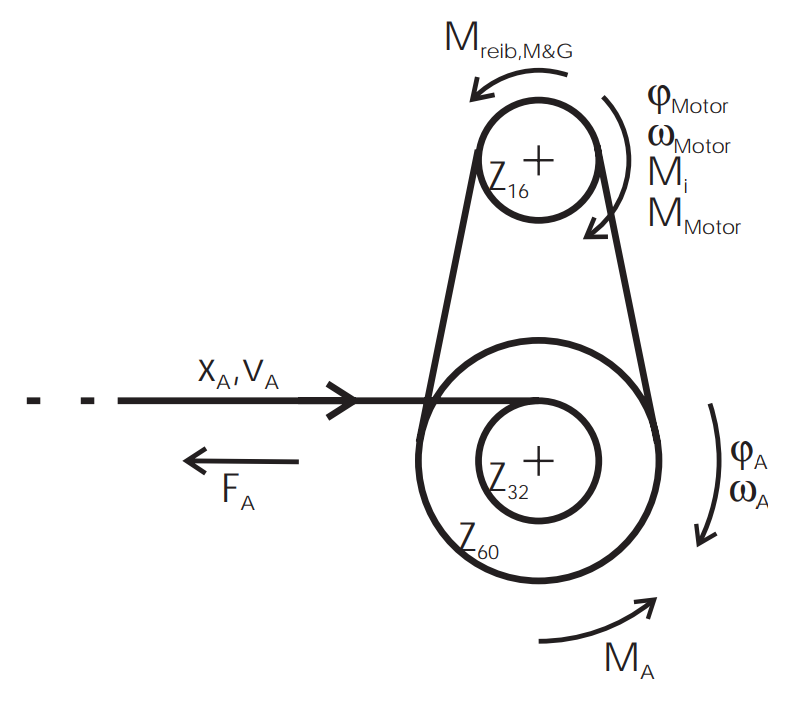
\includegraphics[width=0.50\textwidth]{Bilder/Modellierung/Getriebe.PNG}
	\caption{Getriebe \cite{franke}}
	\label{fig:Getriebe}
\end{figure}

Die Rotorbewegung des Motors wird über das in Abbildung \ref{fig:Getriebe} dargestellte Getriebe und das Antriebszahnrad auf den Zahnriemen weitergegeben. Auf Grund der hohen Steifigkeit des mit eingebetteten Stahlseilen unterstützten Riemens wird dieser wie in Apprich \cite{apprich} als unendlich starr angenommen, sodass die Verbindung von Motor und Schlitten ohne Federkopplung durch eine Übersetzungskonstante modelliert werden kann.
\[
	\dot{x} = K_G \cdot \omega_{Motor}
\]
 Die Übersetzungskonstante $K_G$ zwischen der Winkelgeschwindigkeit des Motors und der Schlittengeschwindigkeit wird über das Zahnverhältnis und den Antriebsradius berechnet.
\[
	K_G =  \frac{Z_{16}}{Z_{60}} \cdot r_{32} .
\]
Der Antriebsradius $r_{32}$ ist dabei der Abstand zwischen der neutralen Phase des Riemens und der Drehachse.


\section{Modellparameter}\label{sec:mparams}

Bevor die in dieser Arbeit verwendeten Parametersätze für Motor- und \spd-Modell vorgestellt werden, soll im folgenden Abschnitt zunächst ein Überblick über die Entwicklung der in den vergangenen Arbeiten verwendeten Modellparameter gegeben werden.  


\subsection{Begründeter Stand der Modellparameter}\label{subsec:paramshist}

Die für die Modellierung erforderlichen Systemparameter des Versuchsstands wurden erstmalig 1997 von Franke \cite{franke} durch Messungen identifiziert. Die Antriebseinheit aus Spannungs-Strom-Wandler, Motor, Getriebe und Riemen ist seitdem nicht verändert worden. Daher repräsentieren die von Franke \cite{franke} identifizierten Modellparameter in Bezug auf die Antriebseinheit weiterhin den aktuellen Stand (siehe \secref{subsec:motorparams})
   
Während zuvor noch ein Einfachpendel verwendet worden war, konstruierte Apprich \cite{apprich} 2009 erstmalig ein Doppelpendel für den Versuchsstand. Von den Änderungen betroffen war neben den Pendeln auch die Schlittenmasse, da auch der obere Teil des Schlittens neu konstruiert wurde. Die Modellparameter für die neuen Pendelstäbe wurden, anders als bei Franke \cite{franke}, nicht gemessen, sondern aus dem CAD-Modell abgeleitet. Dies betrifft die Massen, Trägheitsmomente, Längen und Schwerpunkte der beiden Stäbe. Die Masse des Schlittens wurde von Franke \cite{franke} übernommen. Durch Messungen wurden lediglich die viskose und trockene Reibung des Schlittens gegenüber den Schienen erneut identifiziert. 

Im selben Jahr wurde von Kämmerer \cite{kämmerer} die viskose Lagerreibung $d_1$ zwischen Stab 1 und dem Schlitten als fehlender Modellparameter durch Messungen ergänzt. Die viskose Lagerreibung $d_2$ zwischen Stab 1 und Stab 2 wurde rechnerisch bestimmt, da das Lager gegen Ende der Arbeit getauscht werden musste. Die viskose Dämpfung des Schlittens, die von Apprich \cite{apprich} zuvor gemessen worden war, wurde durch einen deutlich höheren Schätzwert ersetzt. Außerdem wurde erstmalig die Masse von Schlitten und Antrieb zu einer schlittenseitig wirkenden Gesamtmasse zusammengefasst und ebenfalls als Schätzwert ausgewiesen.

Die Reibwerte $d_1$ und $d_2$ wurden 2011 durch Kisner \cite{kisner} erneut bestimmt. Durch die \textit{Prediction-Error Minimization Method} aus der \textit{System Identification Toolbox} von \Matlab\ wurden die Parameter $d_1$ und $d_2$ so variiert, dass die quadratische Fehlersumme minimal wird. Als Fehler ist hierbei die Differenz zwischen den gemessenen und den vom Modell vorhergesagten zeitlichen Winkelverläufen $\varphi_1(t)$ und $\varphi_2(t)$ bei ruhendem Schlitten und frei gewählter Anfangsauslenkung zu verstehen. Für die Optimierung wurden zudem nicht näher beschriebene Anfangsschätzwerte für $d_1$ und $d_2$ gewählt. Es wird davon ausgegangen, dass es sich um Erfahrungswerte handelt, da sie einerseits nicht mit den zuletzt von Kämmerer \cite{kämmerer} bestimmten Werten übereinstimmen, jedoch andererseits zu guten Ergebnissen am Versuchsstand führten. Statt der optimierten Werte wurden in den Nachfolgearbeiten die Anfangsschätzwerte weiterverwendet. Der Reibwert $d_0$ der viskosen Schlittenreibung, der nicht Gegenstand der Optimierung war, wurde mit einem deutlich höheren Wert als bei Kämmerer \cite{kämmerer} angegeben. Da keine explizite Begründung vorliegt, wird von einem Erfahrungswert ausgegangen. Die zuvor von Kämmerer \cite{kämmerer} geschätzte effektive Gesamtmasse von Schlitten und Antrieb wurde nach unten korrigiert, wobei die Hintergründe für diesen Schritt ebenfalls nicht bekannt sind. Der neue Wert ist jedoch plausibel und wird daher ebenfalls als erfahrungsbasierter Schätzwert verstanden. Der ist in den weiteren Arbeiten nicht mehr verändert worden, sodass er als aktueller Stand zu betrachten ist. Bei Kisner \cite{kisner} wurde erstmalig auch eine Begrenzung der Stellkraft von $F_{\mrm{max}}=\valunit{400}{N}$ bezüglich des Schlittens angegeben, die als gegeben dokumentiert ist. 

2011 wurde außerdem von Noupa \cite{noupa} sowohl die viskose als auch die trockene Schlittenreibung gemessen, wobei besonders für die viskose Reibung eine hohe Richtungsabhängigkeit beobachtet wurde. Die gemessenen Werte wurden in den weiteren Arbeiten jedoch nicht weiter beachtet.

Auf Grund eines Austauschs des Lagers von Stab 2 wurde 2014 von Brehl \cite{brehl} eine erneute Identifikation der viskosen Dämpfungskonstanten $d_2$ messungsbasiert durchgeführt. Dabei wurden auch Länge und Masse von Stab 2 gemessen, womit ebenfalls das Massenträgheitsmoment neu berechnet wurde. In den Nachfolgearbeiten wurden jedoch nur die Dämpfungskonstante weiterverwendet, während für Länge, Masse und Trägheitsmoment weiterhin die CAD-Werte von Apprich \cite{apprich} verwendet wurden.  

Chang \cite{chang} konstruierte im Sommersemester 2019 ein neues Doppelpendel, wobei Schlitten und Antrieb nicht verändert worden sind. Die neuen Modellparameter wurden wieder aus dem CAD-Modell abgeleitet. Die Angabe des Schwerpunkts $s_2$ von Stab 2 scheint in der Ausarbeitung jedoch zu fehlen. Die Dämpfungskonstanten $d_1$ und $d_2$ wurden von den Vorgängern übernommen, da bei der Konstruktion die gleichen Rillenkugellager gewählt wurden wie bei Apprich \cite{apprich}. Für $d_1$ wurde der Schätzwert von Kisner \cite{kisner} und für $d_2$ der Messwert von Brehl \cite{brehl} übernommen, wobei in Changs Ausarbeitung versehentlich für beide Parameter Apprich \cite{apprich} als Quelle zitiert wird. Die viskose und die trockene Reibung des Schlittens wurden durch Messung selbst bestimmt. Wie bei Noupa \cite{noupa} wurde bei der viskosen Reibung eine auffällige Richtungsabhängigkeit festgestellt. Die Berücksichtigung der Richtungsabhängigkeit mit einer Vorsteuerung führte jedoch zu einer Verschlechterung des Systemverhaltens. Daher wurde schließlich die linksseitige Dämpfungskonstante für beide Seiten übernommen. Da das neu konstruierte Pendel noch nicht für die weiteren Bestandteile der Arbeit, wie die Auslegung der Regelung und deren Erprobung am Versuchsstand, zur Verfügung stand, wurde weiterhin auf die CAD-Werte von Apprich \cite{apprich} zurückgegriffen. Der Betrag der maximalen Stellkraft $F_{\mrm{max}}$ wurde zudem von dem von Kisner \cite{kisner} zuletzt genannten Wert von \valunit{400}{N} auf \valunit{421}{N} erhöht. Der neue Wert lässt sich rechnerisch nachvollziehen, wie \secref{subsec:motorparams} entnommen werden kann.

Im Rahmen einer Verifikation der von Chang \cite{chang} angegebenen Modellparameter für das neue Doppelpendel, wurden im Wintersemester 2019/2020 durch Ribeiro \cite{ribeiro} die Parameter aus dem CAD-Modell erneut abgeleitet. Da hierbei nicht genauer auf den Anlass der Neubestimmung eingegangen wurde, sich die neu bestimmten Parameter jedoch deutlich von den Vorherigen unterscheiden, wird angenommen, dass sich die von Chang \cite{chang} angegebenen Werte im Rahmen der Verifikation als fehlerbehaftet herausstellt hatten. 
Darüber hinaus wurde durch Messung die Reibung der Pendelgelenke identifiziert. Hierbei wurde neben der viskosen Reibung erstmalig auch die trockene Reibung in den Gelenken ermittelt. Die Parameter von Ribeiro \cite{ribeiro} zu den Pendelstäben sind somit aktueller Stand. Übernommen wurde weiterhin die von Kisner \cite{kisner} geschätzte Gesamtmasse mit Schlitten und Antrieb. Für die maximale Stellkraft wurde im Gegensatz zur Vorgängerarbeit Chang \cite{chang} statt \valunit{421}{N} wieder \valunit{400}{N} angenommen. Es wird vermutet, dass dadurch eine Stellkraftreserve für die Regelung vorgehalten werden sollte.


\subsection{Parameter des Motor-Modells}\label{subsec:motorparams}

Gemäß \secref{subsec:paramshist} werden die Modellparameter für das Motormodell Franke \cite{franke} entnommen. 

Die Steuerspannung $U_{\mrm{Steuer}}$ am Eingang des Spannungs-Strom-Wandlers darf maximal $\pm \valunit{10}{V}$ betragen. Ein Betrag größer als \valunit{10}{V} sollte vermieden werden, da sonst der Impulsstrom über den zulässigen Wert ansteigen und der Stromregler zerstört werden kann.

Die Verstärkung $K_{UI}$ des Spannungs-Strom-Wandlers kann durch ein Potentiometer bis zu einem Wert von etwa \valunit{2}{A/V} eingestellt werden, sodass mit der maximalen Steuerspannung der maximal zulässige Impulsstrom von \valunit{20}{A} erreicht wird. Die zuletzt dokumentierte Einstellung liegt bei
\[
	K_{UI} = \valunit{1,87}{\frac{A}{V}} \ .
\]
Der Wert beinhaltet bereits eine Idealisierung, da Messungen von Franke \cite{franke} gezeigt haben, dass die reale Verstärkung am Versuchsstand eine leichte Richtungsabhängigkeit bezüglich des Vorzeichens aufweist.

Die Zeitkonstante $T_{UI}$ wird als ausreichend klein angesehen, sodass die Dynamik des Wandlers vernachlässigt werden kann.

Alle weiteren verwendeten Parameter des Motormodells sind in \tabref{tab:motorparams} aufgeführt.

\begin{table}[htbp]
	\centering
	\caption{Parameter -- Motorsystem}
		\begin{tabular}{lcc|l}
			\toprule
			Bezeichnung	&	Symbol	&	Einheit	&	Franke97	\\
			\midrule
			Maximale Steuerspannung & $U_{\mrm{Steuer, max}}$ & \unit{V} & 10 \\ 
			Wandlerverstärkung & $K_{UI}$ & \unit{\frac{V}{A}} & 1,87 \\
			Wandlerzeitkonstante & $T_{UI}$ & \unit{s} & 0,00075 \\
			Maximale Ankerspannung & $U_{a \mrm{, max}}$ & \unit{V} & 65 \\
			Ankerwiderstand & $R$ & \unit{\Omega} & 0,9 \\
			Drehmomentkonstante & $K_I$ & \unit{\frac{N m}{A}} & 0,153 \\
			Getriebeübersetzung & $K_G$ & - & $\frac{16}{60}$ \\
			Antriebsradius & $r_{32}$ & \unit{m} & 0,0255 \\			
			\bottomrule
		\end{tabular}
	\label{tab:motorparams}
\end{table}


Mit der statischen Verstärkung zwischen Eingang $U_{\mrm{Steuer}}$ und Ausgang $F$
\begin{align}
	K_{\mrm{MotorGain}} = K_{UI} \cdot K_I \cdot \frac{1}{K_G} \cdot \frac{1}{r_{32}} = \valunit{42,075}{\frac{N}{V}}
	\label{eq:motgain}
\end{align}
lässt sich die maximale Stellkraft
\begin{align}
	F_{\mrm{max}} = U_{\mrm{Steuer, max}} \cdot K_{\mrm{MotorGain}} = \valunit{420,75}{N}
\end{align}
berechnen, wobei $K_{UI} = \valunit{1,87}{A/V}$ ist.
Für $K_{UI \mrm{, max}} = \valunit{2}{A/V}$ läge die maximale Stellkraft bei $F_{\mrm{max}} = \valunit{450}{N}$.

Mit $K_{UI} = \valunit{1,87}{A/V}$ kann zudem
\[
	I_{w\mrm{, max}} = U_{\mrm{Steuer, max}} \cdot K_{UI} = \valunit{18,7}{A} 
\]
berechnet werden, sodass sich mit Hilfe von \equref{eq:wemk} für die Drehzahl, ab der die Gegeninduktion als Strombegrenzung wirksam wird,
\[
	\omega_{\mrm{EMK}} = \valunit{314,84}{\frac{rad}{s}}
\]

ergibt. Dies entspricht nach \equref{eq:kinematik} einer Schlittengeschwindigkeit von $\xop = \valunit{2,14}{\frac{m}{s}}$ 



\subsection{Parameter des Schlittendoppelpendels}\label{subsec:spdparams}

Ausgehend von \secref{subsec:paramshist} werden in dieser Arbeit drei Parametersätze angelegt \siehe{\tabref{tab:spdparams}}.
Dies ermöglicht einen Vergleich der unterschiedlichen Systeme hinsichtlich des Systemverhaltens und der Stabilisierbarkeit.

Aufgrund der Neukonstruktion des \dpd s und dabei aufgetretener Schwierigkeiten in der Regelung ist ein Vergleich zum vorigen System von Interesse.
Die Parameter der alten Konstruktion werden mit \qq{Apprich09} bezeichnet, obwohl hier auch neu bestimmte Werte von Kisner \cite{kisner} und Brehl \cite{brehl} (Reibung und Schlittenträgheit) enthalten sind.
Der zweite Parametersatz \qq{Chang19} stellt die Daten der Ausarbeitung von \cite{chang} dar, in welcher die Neukonstruktion stattfand. 
Da diese erst in der nächsten Arbeit (Ribeiro \cite{ribeiro}) in Betrieb genommen wurde und dort sowohl die CAD-Parameter erneut bestimmt als auch die Reibungsparameter identifiziert wurden, werden die Werte \qq{Ribeiro20} als korrekte Parameter des neukonstruierten \dpd s betrachtet.

\begin{table}[htbp]
	\centering
	\caption{Parameter -- \spds}
		\begin{tabular}{lcc|lll}
			\toprule
			Bezeichnung	&	Symbol	&	Einheit	&	Apprich09	&	Chang19	&	Ribeiro20	\\
			\midrule
			Masse des Schlittens	&	$m_0$	&	\unit{kg}	&	16,5	&	16,5	&	16,5	\\
			Masse des ersten Pendels	&	$m_1$	&	\unit{kg}	& 0,615	&	0,329	&	0,8534	\\
			Masse des zweiten Pendels	&	$m_2$	&	\unit{kg}	&	0,347	&	0,3075	&	0,3957	\\
			Trägheitsmoment des ersten Pendels	&	$J_1$	&	\unit{kg \,m^2}	&	0,00647 &	0,01457	&	0,01128	\\
			Trägheitsmoment des zweiten Pendels	&	$J_2$	&	\unit{kg \,m^2}	&	0,00407	&	0,00334	&	0,003343	\\
			Länge des ersten Pendels	&	$l_1$	&	\unit{m}	&	0,2905	&	0,325	&	0,282	\\
			Länge des zweiten Pendels	&	$l_2$	&	\unit{m}	&	0,3388	&	0,305	&	0,280	\\
			Schwerpunkt des ersten Pendels	&	$s_1$	&	\unit{m}	&	0,0775	&	0,1425	&	0,09373	\\
			Schwerpunkt des zweiten Pendels	&	$s_2$	&	\unit{m}	&	0,146	&	0,114254	&	0,114254	\\
			Viskose Dämpfung des Schlittens	&	$d_0$	&	\unit{\frac{N s}{m}}	&	17	&	17,6	&	17	\\
			Viskose Dämpfung des ersten Pendels	&	$d_1$	&	\unit{\frac{N m s}{rad}}	&	0,0091	&	0,005	&	0,00768	\\
			Viskose Dämpfung des zweiten Pendels	&	$d_2$	&	\unit{\frac{N m s}{rad}}	&	0,0006905	&	0,005	&	0,000285	\\
			\crb\ des Schlittens	&	\Fco	&	\unit{N}	&	16,232	&	17,5	&	13,43	\\
			\crb\ des ersten Pendels	& \Mceo	&	\unit{Nm}	&	0	&	0,0538	&	0,0538	\\
			\crb\ des zweiten Pendels	& \Mczo	&	\unit{Nm}	&	0	&	0,0000912	&	0,0000912	\\
			Erdbeschleunigung	&	$g$	&	\unit{\frac{m}{s^2}}	&	9,81	&	9,81	&	9,81	\\
			\bottomrule
		\end{tabular}
	\label{tab:spdparams}
\end{table}

Es wird somit im Folgenden zwischen den \qq{alten Parametern} (\texttt{Apprich09}) und den \qq{neuen Parametern} (\texttt{Ribeiro20}) unterschieden.
Der größte Unterschied zwischen beiden Systemen ist die \crb\ in den Pendelgelenken, die zusätzlich zur viskosen Reibung erstmals bei Ribeiro \cite{ribeiro} bestimmt wurde.
Da bei der Neukonstruktion die Messsignalübertragung zur Vermeidung einer Kabelaufwickelung über einen Schleifring realisiert wurde, besteht die Vermutung, dass dieser für die erhöhte \crb\ verantwortlich ist. 
Dies macht das System bereits um einen sehr kleinen Arbeitsbereich nichtlinear, was die Regelung erschwert.

Für die Skalierungsparameter \xopth, \pheth\ und \phzth\ der \crb\ \siehe{\secref{sec:crb}} wird jeweils 0,01 angenommen.



\section{Aufbau des Simulationsmodells}

In dieser Arbeit wird das \dpds\ rein simulativ betrachtet.
Das Simulationsmodell wird im Vergleich zu Vorgängerarbeiten wesentlich systematischer und detaillierter aufgebaut.
Dadurch sind umfangreiche und automatisierte Tests möglich, mit denen das System umfassend untersucht werden kann.

Besonders wird in dieser Arbeit Wert auf einen strukturierten, modularen Aufbau gelegt.
Dies soll flexible Änderungen am System, wie \zB Systemparameter oder Reglerparameter ermöglichen.
Von der Berechnung der \bwgl\ über die Parametrisierung des Systems bis zur Reglerberechnung kann das Modell vollständig und konsistent initialisiert werden.
Außerdem soll dadurch die Nutzbarkeit und Wiederverwendbarkeit in zukünftigen Arbeiten gewährleistet sein.

Das Simulationsmodell voriger Arbeiten wie \cite{chang} ist nur wenig strukturiert aufgebaut, enthält Redundanzen und viele fest-kodierte Parameter.
Es wird daher lediglich zur Orientierung verwendet.
Hart-kodierte Parameter werden in dieser Arbeit vermieden, sodass jeder Parameter bei der \init\ geändert werden kann (ohne das \sm-Modell ändern zu müssen).
Auch Gleichungen können variabel ausgelegt werden, was durch die symbolische Schreibweise von \ml\ ermöglicht wird.
Code-Dopplungen werden vermieden. 
Die gesamte \init\ ist stark funktionalisiert, da dies für die Variationstests notwendig ist.
Dadurch wird auch sichergestellt, dass Änderungen nur an einer Stelle vorgenommen werden müssen und automatisch direkt an allen entsprechenden Stellen angepasst werden.

Die \sm-Modelle und \ml-Funktionen zur Modellierung des Systems und \init\ des Simulationsmodells befinden sich im Ordner \texttt{Modell}. 


\subsection{Aufbau in \Simulink}

\subsubsection{Subsysteme}
In \sm\ lassen sich sogenannte \emph{Subsysteme} erstellen, um ein Simulationsmodell übersichtlicher zu gestalten.
Diese Subsysteme (im Folgenden auch Module genannt) lassen sich zudem als Datei externalisieren (\emph{Referenced Subsystem}), wodurch sie einerseits separat bearbeitet werden können und andererseits an mehreren Stellen modular wiederverwendet werden können.
Somit wird lediglich in der obersten Schicht (die Testebene) ein \sm-\emph{Model} verwendet.

In dieser Arbeit werden immer Module erstellt, sofern es sinnvoll erscheint.
Dadurch wird das Gesamtsystem übersichtlich gehalten und kann sehr flexibel modifiziert werden.
Die einzelnen Module (wie \zB Motor, Gesamtmodell, \zsr) stellen zudem wiederverwendbare Teile dar und können so an verschiedenen Stellen im Projekt eingebaut werden, aber möglicherweise auch am \sm-Modell des Versuchsstandes zum Einsatz kommen.
So könnte relativ einfach derselbe Regler an dem echten und dem simulierten System eingesetzt und verglichen werden.

\subsubsection{Maske}
Bei Subsystemen kann eine sogenannte \emph{Maske} eingerichtet werden, wodurch Parameter übergeben werden können.
In deren Abhängigkeit können in einem Subsystem auch initialisierende Berechnungen durchgeführt werden.

Grundsätzlich können in \sm\ alle Variablen aus dem globalen \ml-Workspace verwendet werden, was allerdings fehleranfällig ist.
Geschickter ist es, dem Simulationsmodell eine einzige Variable vom Typ \texttt{struct} zu übergeben, in der alle Parameter vorhanden sind.
So werden jedem Modul über die jeweilige Maske nur genau die Parameter übergeben, von denen es abhängt.
Dadurch bleibt der Gesamtaufbau modularer und strukturierter.

\subsubsection{Scopes und ToWorkspace}
Um die Signalverläufe direkt zu untersuchen, werden an allen wichtigen Stellen in den Simulationsmodellen \emph{Scopes} installiert.
So lässt sich das Systemverhalten oder Probleme in der Regelung schnell und einfach analysieren.
Oft werden Scopes mit mehreren Eingängen verwendet, um Signale besser vergleichen zu können.

Für alle Variablen, die später in \ml\ für weitere Auswertungen zur Verfügung stehen sollen, werden \emph{ToWorkspace}-Blöcke verwendet.
Diese geben die Daten an die Ausgabevariable \texttt{out}.

Für die Screenshots werden diese Blöcke meist aus Übersichtsgründen entfernt.


\subsection{\Simulink\ Module und Modelle}


\subsubsection{Motor.slx}
\begin{figure}[h]
	\centering
		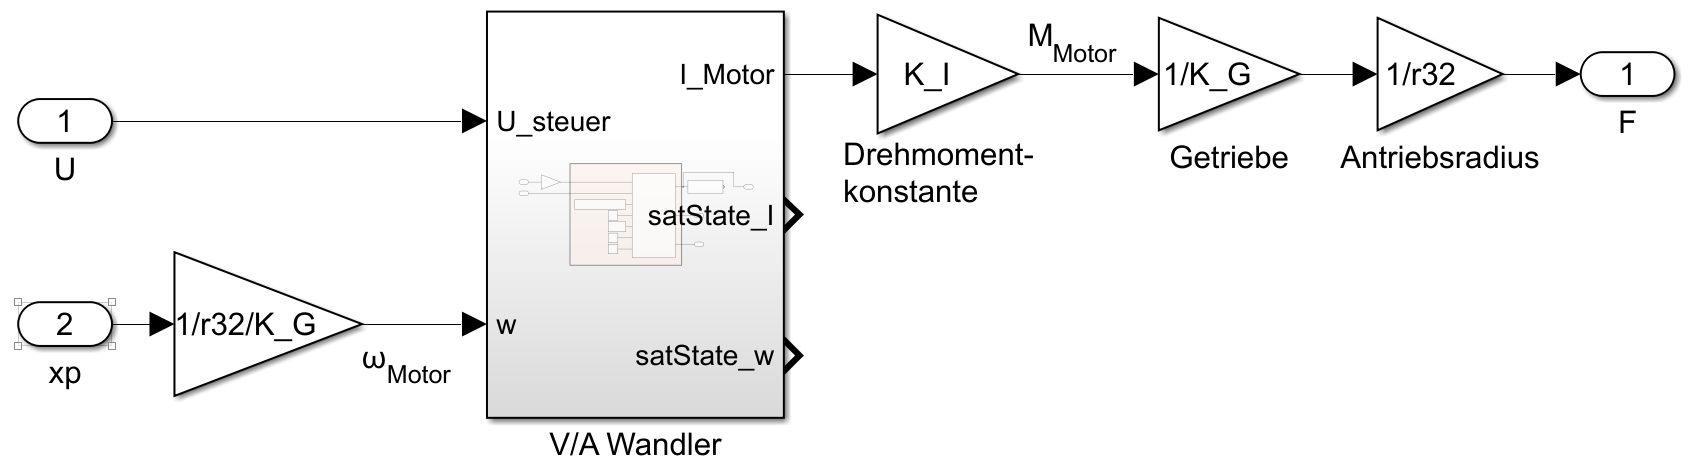
\includegraphics[scale=0.4]{Bilder/Simulink/motor.PNG}
	\caption{Motormodell in \sm}
	\label{fig:simmot}
\end{figure}
Das Motormodell wird \secref{sec:mot} entsprechend als Modul implementiert \siehe{\figref{fig:simmot}}.
Eingangsgröße ist die Steuerspannung sowie die Schlittengeschwindigkeit, da sich daraus die Induktionsspannung ergibt.
Ausgangsgröße ist die Kraft, die am Schlitten wirkt.
Der V/A Wandler wird als Subsystem implementiert und gibt den Motorstrom aus \siehe{\figref{fig:simva}}.
Die Berechnung der Strombegrenzung \siehe{\secref{subsec:dcMotor}} wird als \emph{matlabFunction} realisiert.
Dabei werden die Signale \texttt{satState\_w} (falls die Sättigungsdrehzahl erreicht ist) und \texttt{satState\_I} (falls der Sollstrom nicht erreicht werden kann) gesetzt und können später analysiert werden.
Die Tiefpass-Charakteristik der Induktivität wird mit dem \mrm{PT_1}-Glied \eqref{eq:UI} dargestellt.


\begin{figure}
	\centering
		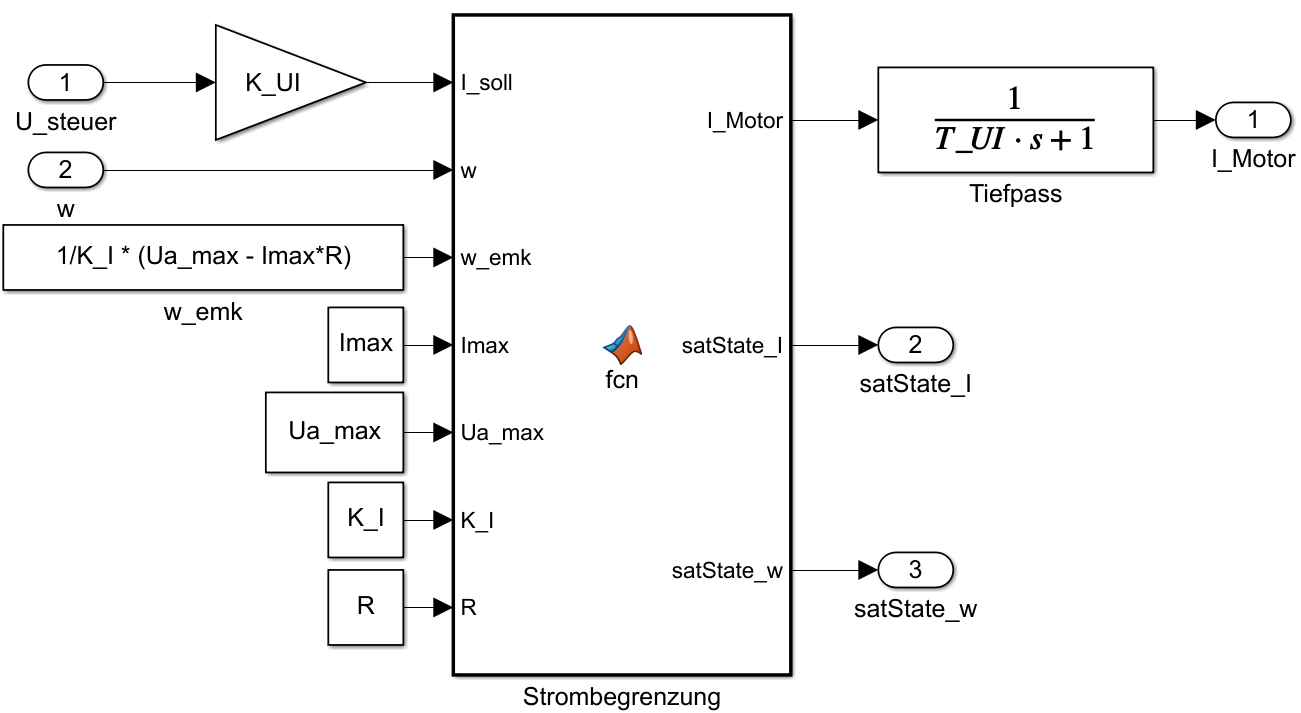
\includegraphics[scale=0.4]{Bilder/Simulink/va_wandler.PNG}
	\caption{V/A Wandler in \sm}
	\label{fig:simva}
\end{figure}

\subsubsection{SchlittenPendel.slx}
Das \zrm\ des \spds s wird mit einer \emph{S-Function} dargestellt.
Die zugehörige \ml-Datei \texttt{SchlittenPendelFunc.m} wird automatisch bei der \init\ erstellt \siehe{\secref{subsec:init}}.
Lediglich die Anfangswerte werden über die Simulationsparameter übergeben.

\subsubsection{Gesamtmodell.slx}\label{sec:gesamtslx}
Dieses Modul stellt das gesamte Modell dar und fasst die beiden vorigen Module zusammen \siehe{\figref{fig:simges}}.
Die Eingangsspannung wird an den Motor gegeben und dessen Ausgang $F$ ist die Schnittstelle zum \sdpd.
Die Schlittengeschwindigkeit wird zum Motor zurückgeführt, da durch diese die Motordrehzahl bestimmt wird.

\begin{figure}[h]
	\centering
		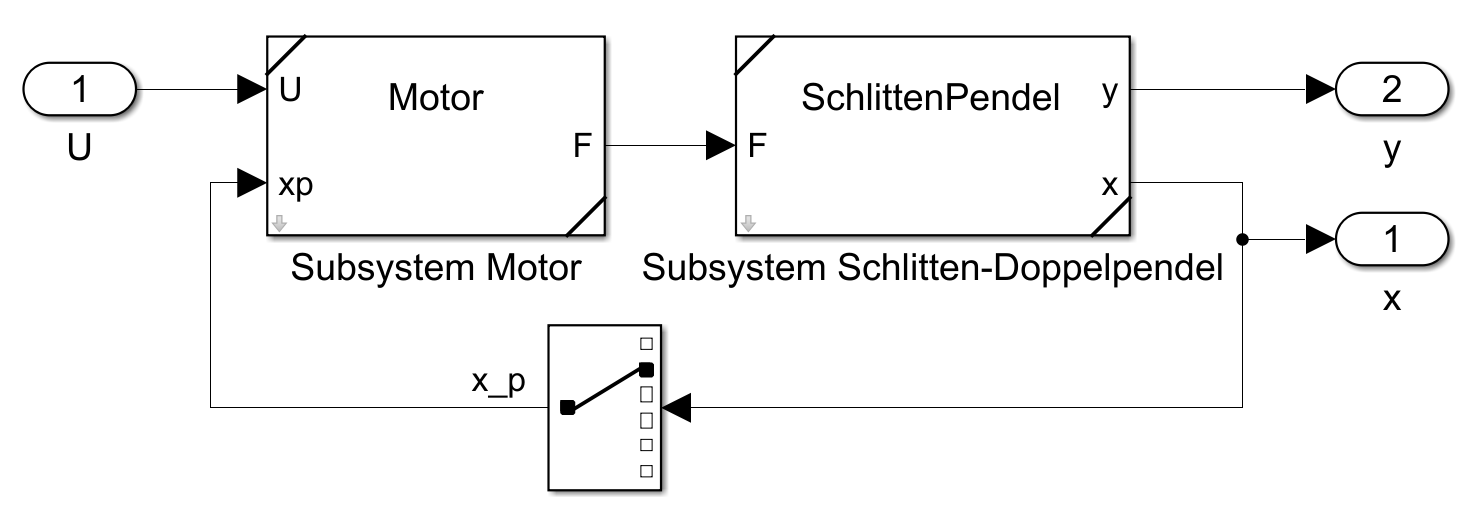
\includegraphics[scale=0.4]{Bilder/Simulink/gesamtmodell.PNG}
	\caption{Gesamtmodell in \sm}
	\label{fig:simges}
\end{figure}

\subsubsection{Gesamtmodell\_Test.slx}
Dies ist ein \sm-Modell und bindet das Gesamtmodell-Modul ein.
Auf dieses können testweise verschiedene Eingangsverläufe gegeben werden, um das Systemverhalten auf Plausibilität zu überprüfen, beispielsweise:
\begin{itemize}
	\item Keine Spannung, aber Anregung durch Anfangsauslenkung
	\item Konstante Spannung
	\item Sinusförmige Spannung
\end{itemize}
Da die durchgeführten Tests am Modell plausible Ergebnisse zeigen, wird im Folgenden von der Korrektheit des Simulationsmodells ausgegangen.


\subsection{Parameter}

Größere zusammenhängende Parameterdaten werden als Datei \bzw Funktion ausgelagert, um eine einfache Austauschbarkeit zu erreichen.
Die drei Parametersätze des \spd s \siehe{\tabref{tab:spdparams}} sowie die Motorparameter befinden sich im Ordner \path{Modellparameter}.


\subsection{Initialisierung}\label{subsec:init}

Zum Initialisieren des Modells und der Simulation führt man das Skript \texttt{Init.m} aus.
Dadurch werden folgende 4 Schritte durchgeführt:
\begin{enumerate}
	\item \textbf{InitSymEq}: Berechnet symbolisch die \bwgl\ nach \secref{subsec:bwgl} für das \krs\ (\path{SchlittenPendelSymF}) und das \bss\ (\path{SchlittenPendelSymA}) und speichert sie als globale Variablen. Auch die Ruhelagen werden initialisiert (definiert in\break \path{SchlittenPendelRuhelagen}).
	\item \textbf{InitParams}: Initialisiert die Parameter des Motors und des Schlittens (standardmäßig \texttt{Ribeiro20}) als globale Variablen. Hier können die Parameter ausgetauscht oder verändert werden (\zB \crb\ abschalten).
	\item \textbf{InitSystem(SchlittenPendelParams)}: Diese Funktion erstellt die \zrm e des\break \spds s nach \secref{subsec:zrm}. Dafür wird die Funktion \mbox{\path{SchlittenPendelNLZSR.m}} genutzt, welche das \zrm\ in Abhängigkeit der \bwgl\ und der Parameter erstellt. Aus dem \krs\ wird mittels \path{sys2sfct} eine \emph{S-Function} generiert und in \path{SchlittenPendelFunc.m} gespeichert.
	\item \textbf{InitSim}: Bereitet die globale Variable \path{simparams} vor, in welcher alle Parameter für das \sm-Modell übergeben werden. Dazu gehören beim Modell die Motorparameter und die Startwerte des \spds s.
\end{enumerate}
Nach der \init\ kann \path{Gesamtmodell_Test.slx} ausgeführt werden.


\subsection{Auswertung}\label{subsec:ausw}

Nach einer Simulation ist es nützlich, die wesentlichen Ergebnisse direkt ablesen zu können (\zB ob der Schlitten außerhalb der Begrenzung war oder ob der Motor in Sättigung war).
Außerdem wird eine Plot-Funktion implementiert, die die wichtigsten Verläufe darstellt.
Um das Verhalten des \dpd s besser interpretieren zu können, wird zudem eine Animationsfunktion erstellt, die direkt das Pendelverhalten visualisiert.

Die entsprechenden \ml-Funktionen sind im Ordner \path{Auswertung} vorhanden.
Weitere Informationen und Kommentare finden sich auch meist in den \ml-Funktionen selbst.

\subsubsection{plot\_outputs}
Erstellt ein Diagramm, dass die drei Verläufe der Ausgangsgrößen (inklusive deren Schätzwerte) und die Stellgröße (Soll- und Ist-Wert) darstellt.
Der Funktion können einige Parameter übergeben werden, sodass das Diagramm auch abgespeichert werden kann.
Für weitere Informationen sei auf die Dokumentation in der Datei \path{plot_outputs.m} verwiesen.

\subsubsection{animate\_outputs}
Stellt die Bewegungen des Schlittens und des \dpd s zeitlich dar.
Parameter für die Bildwiederholrate (FPS) und ein Zeitfaktor können angegeben werden.
Außerdem kann das Video gespeichert werden.
Für mehr Informationen siehe \path{animate_outputs.m}.

\subsubsection{plotanimate}
Führt die beiden obigen Funktionen aus, sodass Ergebnisse mit einem Funktionsaufruf gemeinsam gespeichert werden können.
Beispiel:
	\[
	\texttt{plotanimate(out, 'u=0,AP4,phi2=0.01', 'Modell Tests', 60, 1/4 )}
\]


%\subsection{Weitere \Matlab-Funktionen}



\chapter{Arbeitspunkt-Regelung}\label{cha:apr}

Nachdem im letzten Kapitel die Modellierung des Gesamtsystems erläutert wurde, stellt sich nun Frage, wie sich das System regeln lässt. Dabei geht es einerseits um die Regelung an den 4 Arbeitspunkten \secref{sec:aps} sowie um \traj n, die das \dpd\ von einem \ap\ in einen anderen überführen.

\section{Vorgehen}%\label{sec:}

Beim Reglerentwurf wird zunächst dem Vorgehen vergangener Arbeiten gefolgt. 

\subsection{\lin}\label{subsec:lin}

Da das \zrm\ des \spds s \eqref{eq:zrm} nicht-linear ist, muss es um jeden \ap\ linearisiert werden, bevor lineare Regelungsmethoden angewandt werden können. 
\begin{align}
	\mat{A} &= \left. \frac{\partial \vef(\vex,u_R)}{\partial \vex} \right|_{\vex=\vexr}  
		= \left. \begin{bmatrix}
		0 & 1 & 0 & 0 & 0 & 0 \\
		0 & \partiald{a_2(\vex)}{\xop} & \partiald{a_2(\vex)}{\phe} & \partiald{a_2(\vex)}{\phep} & \partiald{a_2(\vex)}{\phz} & \partiald{a_2(\vex)}{\phzp} \\
		0 & 0 & 0 & 1 & 0 & 0 \\
		0 & \partiald{a_4(\vex)}{\xop} & \partiald{a_4(\vex)}{\phe} & \partiald{a_4(\vex)}{\phep} & \partiald{a_4(\vex)}{\phz} & \partiald{a_4(\vex)}{\phzp} \\
		0 & 0 & 0 & 0 & 0 & 1 \\
		0 & \partiald{a_6(\vex)}{\xop} & \partiald{a_6(\vex)}{\phe} & \partiald{a_6(\vex)}{\phep} & \partiald{a_6(\vex)}{\phz} & \partiald{a_6(\vex)}{\phzp} \\
	\end{bmatrix} \right._{\vex=\vexr}  \\
	\mat{B} &= \left. \frac{\partial \vef(\vex_R,u)}{\partial u} \right|_{u=u_R}
	= \ve{b}(\vexr) = \begin{bmatrix}
		0 \\ b_2(\vexr) \\ 0 \\  b_4(\vexr) \\ 0 \\  b_6(\vexr)
	\end{bmatrix}
\end{align}
Somit ergeben sich für jeden \ap\ unterschiedliche Systemmatrizen \mat{A} und Eingangsmatrizen \ve{B}. Beim \bss\ fällt zusätzlich die zweite Zeile und die zweite Spalte (bis auf die 1) weg, da dort $a_2=0$ ist und keine Abhängigkeit von \xop\ besteht (siehe \tabref{tab:abh}), außerdem ist $b_2=1$.
Die Ausgangsmatrix \mat{C} ist immer gleich, da die Ausgangsgleichung \eqref{eq:hx} linear ist.


\subsection{Eigenwerte}

Anhand der \ewe\ können Aussagen über die Dynamik eines Systems getroffen werden. 
Beim \bss\ gibt es aufgrund der zweifachen Integration des Eingangs \xopp\ stets zwei \ewe\ in 0. 
Mit den Apprich-Parametern ergeben sich folgende \ewe:
\begin{table}[htbp]
	\centering
		\begin{tabular}[t]{cccc}
			\toprule
			\ape & \apz & \apd & \apv \\
			\midrule
			$0$	&	$0$	&	$0$	&	$0$	\\
			$0$	&	$0$	&	$0$	&	$0$	\\
			$-0.2972 +11.4177\iu$ &    $7.8028						$	&	  $6.8596							$	&   $11.1308$	\\
			$-0.2972 -11.4177\iu$ &   $-7.9367						$	&   $-7.2314					$		&  $-11.7251$	\\
			$-0.0418 + 4.8515\iu$ &   $-0.1858 + 7.0392\iu$	&  $-0.0669 + 7.8676\iu$	&  $  4.8089$	\\
			$-0.0418 - 4.8515\iu$ &   $-0.1858 - 7.0392\iu$	& $ -0.0669 - 7.8676\iu	$	&  $ -4.8926$	\\
			\bottomrule
		\end{tabular}
	\caption{\ewe\ des \bss s (Parameter: Apprich)}
	\label{tab:ewappr}
\end{table}

Im \ap\ 1 ergeben sich zwei konjugiert-komplexe Polpaare, die sich physikalisch mit der Schwingung der beiden Pendel begründen lassen. Sie befinden sich aufgrund der Dämpfung in der linken s-Halbebene, es ist der einzige stabile \ap. \ap\ 2 und 3 besitzen jeweils ein konjugiert-komplexes Polpaar, da dort das erste \bzw zweite Pendel nach unten zeigt und damit \qq{stabil} ist. Der Realteil ist bei \ap\ 3 deutlich kleiner, was auf die geringere Dämpfung des zweiten Pendelgelenks zurückzuführen ist (siehe \tabref{tab:parappr}). Aufgrund der Instabilität des anderen Pendels ergibt sich jeweils ein positiv reeller \ew. In \ap\ 4 stehen beide Pendel oben, weswegen es dort zwei \ewe\ in der rechten s-Halbebene gibt.

\begin{table}[htbp]
	\centering
		\begin{tabular}[t]{cccc}
			\toprule
			\ape & \apz & \apd & \apv \\
			\midrule
				$0$	&	$0$	&	$0$	&	$0$	\\
				$0$	&	$0$	&	$0$	&	$0$	\\
				$-174.3727$						&	$-172.9211$	&	$-173.2473$						&	$-175.4362$	\\
				$-0.3493$							&	$-0.3494$		&	$0.3471$							&	$0.3471$	\\
				$-0.6385 + 7.1578\iu$	&	$6.7715$		&	$-0.6443 + 7.2040\iu$	&	$6.7469$	\\
				$-0.6385 - 7.1578\iu$	&	$-7.6900$ 	&	$-0.6443 - 7.2040\iu$ &	$-7.6570$ \\
			\bottomrule
		\end{tabular}
	\caption{\ewe\ des \bss s (Parameter: Ribeiro)}
	\label{tab:ewribe}
\end{table}

Mit den neuen Parametern (Ribeiro) ergibt sich ein anderes Bild (siehe \tabref{tab:ewribe}).
Bei \ap\ 1 und 2 verschwindet ein Polpaar, welches dem ersten Pendel zugeordnet wurde. Ein sehr schneller \ew\ kommt hinzu, außerdem ein langsamer reeller, der bei \ap\ 3 und 4 positiv ist. 
Die Ursache für diese Änderung liegt vermutlich in der Modellierung der \crb\ (siehe \secref{sec:crb}). Bei der \lin\ um die Ruhelage wird die Annäherungsfunktion der \mrm{signum}-Funktion um 0 linearisiert, wo sie sehr steil ist. Dies resultiert in einer sehr hohen Dämpfung. Daher ist es sinnvoll, die \crb\ der Pendelstäbe für den AP-Reglerentwurf zu vernachlässigen.
Wird die \crb\ zu 0 gesetzt, ergeben sich prinzipiell ähnliche Werte wie in \tabref{tab:ewappr}.


\subsection{Steuerbarkeit und Beobachtbarkeit}

Voraussetzung für eine Regelung ist die Steuerbarkeit des Systems. Diese kann für lineare Systeme oder linearisierte Systeme an einem \ap\ mit dem Steuerbarkeitskriterium nach Kalman überprüft werden \cite{AdamyRT2}. Außerdem sollte ein System beobachtbar sein, falls nicht alle Zustände bekannt sind und daher über einen Beobachter ermittelt werden.

Das \spds\ (\bss) ist an allen 4 \ap en vollständig steuer- und beobachtbar.


\subsection{Zustandsregler}\label{subsec:zsr}

Die \aprg\ wird mit einem \zsr\ realisiert. Die Verstärkung $K$ wird durch Lösen des LQ-Problems ermittelt \cite{AdamyRT2}. Parameter für den Entwurf sind somit die Matrix \mat{Q} zur Bewertung der Zustände und $R$ für die Stellgröße. 

Für jeden \ap\ muss ein eigener Regler entworfen werden. 




\section{Aufbau in \Simulink}



\section{Implementierung in \Matlab}



\section{Anfangswert-Tests}

\begin{figure}
	\centering
	\begin{minipage}[t]{0.45\linewidth}
		\centering
		\includegraphics[scale=0.5]{Bilder/Parameter neu (Ribeiro) Creg off/AP2.pdf}
		%\caption{\ap  2}
		\label{fig:ap2}
	\end{minipage}
	\hfill
	\begin{minipage}[t]{0.45\linewidth}
		\centering
		\includegraphics[scale=0.5]{Bilder/Parameter neu (Ribeiro) Creg off/AP3.pdf}
		%\caption{\ap  3}
		\label{fig:ap3}
	 \end{minipage}
	\\
	\begin{minipage}[t]{0.45\linewidth}
		\centering
		\includegraphics[scale=0.5]{Bilder/Parameter neu (Ribeiro) Creg off/AP41.pdf}
		%\caption{\ap  3}
		\label{fig:ap3}
	 \end{minipage}
	\hfill
	\begin{minipage}[t]{0.45\linewidth}
		\centering
		\includegraphics[scale=0.5]{Bilder/Parameter neu (Ribeiro) Creg off/AP42.pdf}
		%\caption{\ap  3}
		\label{fig:ap3}
	 \end{minipage}
	\caption{Vergleich QR-Parameter (System Ribeiro)}
%\vspace{15pt}
\end{figure}




\section{QR Parameter Tests}



\section{System Parameter Tests}




\chapter{Trajektorien}\label{cha:trj}

%bei der TFR?
Da es bei der Trajektorienfolgeregelung aufgrund der Beschränkung einiger Systemzustände immer wieder zu Schwierigkeiten bei der Berechnung und Umsetzung von Trajektorien kam, wurde durch Fauvé \cite{fauve} der Ansatz der Modellprädiktiven Regelung (engl.: \textit{Model Predictive Control}, MPC), die im Gegensatz zu den klassischen Regelungsverfahren eine Berücksichtigung der Systembeschränkungen ermöglicht, für das bestehende Pendelsystem untersucht. Obwohl sich der Ansatz aufgrund ungenügender Echtzeitfähigkeit nicht für die Regelung eignete, erwies er sich in Bezug auf die Berechnung von Trajektorien für Arbeitspunktwechsel als vielversprechend. 
%Erste Versuche, die erfolgreich berechneten Trajektorien in der Simulation mit Hilfe einer Trajektorienfolgeregelung zu stabilisieren, gelangen jedoch nicht. Daher bleibt zu zeigen, dass die mittels NMPC gefundenen Trajektorien am System stabilisiert werden können. Zudem wird vermutet, dass neben der Regelbarkeit auch das Finden von Trajektorien durch die Systemparameter beeinflusst wird. 
% zu spezifisch für Einleitung


\section{Trajektorienberechnung}

Die Implementierung der Trajektorienberechnung basiert auf den Erkenntnissen der Vorgängerarbeit Fauvé \cite{fauve} und erfolgt in \Matlab\ mit Hilfe des \casadi-Frameworks \cite{Andersson2019}. Es wird einerseits auf eine Erhöhung der Modularisierung im Vergleich zur Vorgängerarbeit geachtet, andererseits werden weitere Funktionalitäten ergänzt, um die Trajektorienberechnung für die Anwendungen im Rahmen dieser Arbeit und die zukünftige Weiterverwendung zu optimieren.

Die Berechnung der Trajektorien wird durch fünf Matlab-Funktionen modularisiert:
\begin{itemize}
	\item \texttt{searchTrajectories}
	\item \texttt{calculateTrajectory}
	\item \texttt{getODE}
	\item \texttt{getInitDev}
	\item \texttt{determineAPinit}
\end{itemize}

Vom Anwender aufgerufen wird lediglich \texttt{searchTrajectories}. Die weiteren vier Funktionen werden auch für andere Anwendungen dieser Arbeit eingesetzt, wodurch das Kopieren von Code vermieden wird. Änderungen, die mehrere Funktionen und Skripte betreffen, können daher effizient an einer Stelle im Programmcode durchgeführt werden. Die Argumente der Funktionen werden so gewählt, dass die in dieser Arbeit zu untersuchenden Parameter leicht durch den Funktionsaufruf in einer Schleife variiert werden können. Weitere Parameter die im Rahmen dieser Arbeit innerhalb der Funktionen konstant festgelegt sind, können zu einem späteren Zeitpunkt jedoch leicht zu den Funktionsargumenten ergänzt werden.

Die implementierten Werkzeuge zur Trajektoriensuche eignen sich für eine weitere Verwendung in zukünftigen Arbeiten. Obwohl im Rahmen dieser Arbeit in erster Linie eine definierte Vergleichstrajektorie verwendet wird, ist eine systematische Suche für alle zwölf Trajektorien im Sinne zukünftiger Anwendungen vorgesehen. Diese wurde im Rahmen dieser Arbeit erfolgreich durch eine Reproduktion der Ergebnisse von Fauvé \cite{fauve} getestet.

Im Folgenden werden die wichtigsten Funktionen \texttt{searchTrajectories} und \texttt{calculateTrajectory} genauer beschrieben, wobei auch auf die Verwendung der anderen Funktionen eingegangen wird.




\subsection{searchTrajectories}\label{subsec:searchtrj}

Durch die Funktion \texttt{searchTrajectories} wird vom Anwender eine Trajektoriensuche in Auftrag gegeben. Als Beispiel für die Anwendung kann der folgende Programmcode eines \Matlab-Skriptes betrachtet werden:

\lstinputlisting[style=Matlab_colored]{Bilder/Trajektorien/Demo_searchTrajectories.m}

Zunächst wird ein Suchprogramm ausgewählt. Es kann zwischen den drei Programmen

\begin{enumerate}
	\item Suche nach der im Rahmen dieser Arbeit definierten Vergleichstrajektorie
	\item Suche nach der Aufschwungtrajektorie mit der Variationsstrategie
	\item Suche nach allen 12 Trajektorien mit der Variationsstrategie
\end{enumerate}

ausgewählt werden.

Dem Ansatz der Programmauswahl liegen die Erkenntnisse von Fauvé \cite{fauve} bezüglich einer Variationsstrategie zu Grunde. Da auf Grund der nichtlinearen MPC nur lokal optimiert wird, kann je nach Anfangswert ein anderes Optimum erreicht werden. Eine Variation des Anfangswertes ermöglicht somit eine effektive Suche nach Trajektorien für einen bestimmten Arbeitspunktwechsel. Im Code-Beispiel ist Suchprogramm 2 ausgewählt, der gesuchte Arbeitspunktwechsel ist allgemein der Aufschwung von AP1 nach AP4. Hierbei können innerhalb einer Periode vier mögliche Winkelanfangsauslenkungen gegenüber AP4 variiert werden, die als Startwert AP1 definieren:
\[
	\begin{bmatrix}
		0 \\ 0 \\ \pi \\ 0 \\ \pi \\ 0
	\end{bmatrix}, \quad
	\begin{bmatrix}
		0 \\ 0 \\ -\pi \\ 0 \\ \pi \\ 0
	\end{bmatrix}, \quad
	\begin{bmatrix}
		0 \\ 0 \\ \pi \\ 0 \\ -\pi \\ 0
	\end{bmatrix}, \quad
	\begin{bmatrix}
		0 \\ 0 \\ -\pi \\ 0 \\ -\pi \\ 0
	\end{bmatrix} .
\]
Eine weitere Variation durch Ausnutzung der $2\pi$-Periodizität bringt gemäß Fauvé \cite{fauve} hingegen keine Vorteile, sondern verlängert die Berechnungszeit bei gleichzeitig sinkender Wahrscheinlichkeit, dass der Algorithmus zu einer gültigen Lösung konvergiert. Die möglichen Anfangsauslenkungen werden über die Funktion \texttt{getInitDev} aufgerufen.
Neben den Anfangsauslenkungen der Pendel hat auch die Schlittenposition Einfluss auf die Lösungsfindung. Daher wird diese mit den folgenden auf Fauvé \cite{fauve} basierenden Auslenkungen symmetrisch zur Bahnmitte variiert (siehe \tabref{tab:varpos}).
\begin{table}[h]
	\centering
	\caption{Variation der Schlittenposition}
		\begin{tabular}{r|l}
			$x_{0\mrm{,init}}$ & $x_{0\mrm{,end}}$ \\
			\midrule
			$-0,5$ & $0,5$	\\	
			$-0,3$ & $0,3$	\\	
			$-0,1$ & $0,1$	\\	
			   $0$ &   $0$	\\
			
		\end{tabular}
	\label{tab:varpos}
\end{table}

Als letzte Komponente der Variationsstrategie wird noch die Positionsbeschränkung variiert. Obwohl der Versuchsstand eine Positionsbeschränkung von $\pm\valunit{0,8}{m}$ vorgibt, ist es sinnvoll, auch diese zu variieren, da der Algorithmus sich sensitiv gegenüber den Nebenbedingungen verhält. Durch Verschärfung oder Lockerung der Positionsbeschränkung verändert sich die Optimierungslandschaft und damit die Chance, eine Trajektorie zu finden. Bei Lockerungen der Beschränkung muss später immer geprüft werden, ob bei den gefundenen Trajektorien die Positionsbeschränkungen eingehalten werden. Es werden folgende von Fauvé \cite{fauve} entnommene Variationen implementiert.
	\[
	-\underline{g}_{x_0} = \overline{g}_{x_0} \in \{ 0,6; \ 0,8; \ 1; \ 1,2; \ 1,4 \}  
\]
Insgesamt werden bei Suchprogramm 2 somit $4 \cdot 4 \cdot 5 = 80$ Trajektorienberechnungen durchlaufen. Bei Suchprogramm 3 werden die beschriebenen Variationen auf alle zwölf Trajektorien ausgeweitet, indem der Endwert durch alle vier Arbeitspunkte iteriert und die Variation der Winkelanfangsauslenkungen um die vier zusätzlich entstehenden Kombinationen durch die Arbeitspunkte 2 und 3 erweitert wird. Insgesamt werden $8 \cdot 4 \cdot 5 \cdot 4 = 640$ Trajektorienberechnungen durchgeführt.
Im Rahmen dieser Arbeit wird eine Vergleichstrajektorie für die in Kapitel \ref{sec:trjparamtest} behandelten Parameteruntersuchungen verwendet. Diese wird mit Suchprogramm 1 berechnet.

Nachdem das Suchprogramm für die Trajektorienberechnung ausgewählt ist, werden Prädiktionshorizont, Schrittweite und Integrationsverfahren für die NMPC konfiguriert. Als Integratoren stehen das Eulerverfahren "`Euler"' und das Runge-Kutta-Verfahren "`RK4"' zur Verfügung. Außerdem wird einer der in Kapitel \ref{subsec:spdparams} besprochenen Parametersätze übergeben sowie eine maximale Stellkraft definiert. Diese stellt eine weitere Variationsmöglichkeit dar, die von Fauvé \cite{fauve} nicht untersucht worden ist. Daher wird sie zur manuellen Variation in den Argumenten der \texttt{searchTrajectories} zur Verfügung gestellt.
Als Letztes wird noch bestimmt, ob für die Trajektorienberechnung die Coulomb-Reibung im Schlitten bzw. in den Gelenken berücksichtigt werden soll. 

Die berechneten Trajektorien werden automatisch gespeichert. Es wird eine Namenskonvention zur Identifizierbarkeit der gespeicherten Ergebnisse eingeführt, die an folgendem Trajektoriennamen beispielhaft gezeigt wird: \texttt{Traj14\_dev0\_-3.14\_-3.14\_x0max0.8\_Fmax410} \ .

Am Anfang steht die verallgemeinerte Trajektorienbezeichnung mit $\mrm{AP_{init}}$ und $\mrm{AP_{end}}$, wobei $\mrm{AP_{init}}$ erst noch aus den Anfangsauslenkungen abgeleitet werden muss. Dies geschieht mit Hilfe der Funktion \texttt{determineAPinit}. Es folgen der Variationswert der Schlittenposition, die Winkelanfangsauslenkung von $\varphi_1$ und $\varphi_2$, die Positionsbeschränkung und die maximale Stellkraft. 
Wenn nicht anders angegeben, werden die Ergebnisse im Ordner \texttt{searchResults} in einer definierten Ordnerstruktur gespeichert, deren Benennung sich nach der Konfiguration der NMPC richtet. Im obigen Beispiel werden die Ergebnisse in folgendem Unterordner gespeichert, wobei \texttt{Fc} anzeigt, dass die \crb\ des Schlittens in der Berechnung berücksichtigt wurde: \texttt{Results\_app09\_Fc\_T0.005N500\_RK4} \ .

Optional kann der Funktion \texttt{searchTrajectories} auch ein Pfad für den Speicherordner übergeben werden. Außerdem können zusätzliche Erweiterungen für den Trajektoriennamen übergeben werden, um später bei der Variation von Modellparametern die Variationswerte im Dateinamen zu berücksichtigen. 
Als weitere Option kann noch bestimmt werden, ob alle berechneten Trajektorien oder nur die mit gültiger Lösung gespeichert werden sollen. 







\subsection{calculateTrajectory}\label{subsec:calctrj}

Die Funktion \texttt{calculateTrajectory} wird innerhalb von \texttt{searchTrajectories} zur eigentlichen Berechnung einer bestimmten Trajektorie aufgerufen. Sie implementiert die NMPC mit Hilfe des \casadi-Frameworks auf Grundlage der Erkenntnisse der Vorgängerarbeit. Für detaillierte Hintergrundinformationen wird daher auf die Ausarbeitung von Fauvé \cite{fauve} verwiesen. Als Argument erwartet die Funktion eine Struktur mit verschiedenen Konfigurationsparametern, die im Quelltext ausführlich kommentiert sind. Da die Funktion \texttt{calculateTrajectory} eigens für die Trajektorienberechnung vorgesehen ist, wird, anders als bei Fauvé \cite{fauve}, auf die Implementierung einer Iterationsschleife für die Anwendung als Regler verzichtet.

\subsubsection{Zielfunktion}

Zunächst muss ein Optimalsteuerungsproblem (OCP) mit Zielfunktion und Nebenbedingungen definiert werden. Als Zielfunktion wird 
	\[
	J = \sum_{i=1}^N \left((x_i-x_\mrm{end})^\transp \mat{Q} (x_i-x_\mrm{end}) + (u_i-u_\mrm{end})^\transp R (u_i-u_\mrm{end})\right) + 
	\sum_{i=2}^N (u_i-u_{i-1})^\transp S (u_i-u_{i-1})
\]
implementiert. Sie besteht aus dem bekannten \emph{Lagrange'schen} Güteintegral der LQ-Regelung und einem Bestrafungsterm für Änderungen in der Stellgröße, durch den hochfrequente Stellgrößenverläufe reduziert werden. Die Wahl der Gewichtungsmatrizen $\mat{Q}$, $R$ und $S$ basiert auf den Erkenntnissen von Fauvé \cite{fauve}. Tests bestätigen diese Wahl, wobei $S$ etwas nach unten korrigiert wird. Die Matrizen werden anschließend nicht mehr variiert. Sie sind der Funktion \texttt{calculateTrajectory} als Konfigurationsparameter zwar zu übergeben, werden in \texttt{searchTrajectories} jedoch für die weiteren Anwendungen im Rahmen der Arbeit hartkodiert.
\[ 
	\mat{Q} = 
	\begin{bmatrix}
		500 & 0 & 0 & 0 & 0 & 0 \\
		0 & 0,01 & 0 & 0 & 0 & 0 \\
		0 & 0 & 100 & 0 & 0 & 0 \\
		0 & 0 & 0 & 0,1 & 0 & 0 \\
		0 & 0 & 0 & 0 & 100 & 0 \\
		0 & 0 & 0 & 0 & 0 & 0,1 \\
	\end{bmatrix} \ , \quad
	R = 5 \cdot 10^{-7} \ , \quad
	S = 1,5 \cdot 10^{-8} \\	
\]

\subsubsection{Nebenbedingungen}

Neben der Zielfunktion sind darüber hinaus folgende Nebenbedingungen zu implementieren:
\begin{itemize}
	\item Kontinuitätsbedingungen 
	\item Anfangsbedingung
	\item Endwertbedingung
	\item Positionsbegrenzung des Schlittens
	\item Stellkraftbegrenzung
\end{itemize}

Dabei ist zu beachten, dass die Endwertbedingung, anders als die restlichen Nebenbedingungen, nicht als harte Grenze formuliert, sondern implizit durch die Zielfunktion angenähert wird. 

Um eine möglichst hohe Vergleichbarkeit mit der Vorgängerarbeit Fauvé \cite{fauve} zu erzielen, wird für die Systemgleichungen das Kraftmodell  \eqref{eq:zrmF} gewählt. Die nichtlinearen Gleichungen werden mit Hilfe der Funktion \texttt{getODE} in \casadi-Symbolik zur Verfügung gestellt.

Die Stellstrombegrenzung in Abhängigkeit der Winkelgeschwindigkeit des Motors wird in \secref{subsec:dcMotor} hergeleitet. Diese muss für die Implementierung noch in eine Stellkraftbegrenzung in Abhängigkeit der Schlittengeschwindigkeit umgerechnet werden.
Mit 
	\[
	\omega = \frac{1}{r_{32}\ K_G} \ \dot{x}_0 
\]
und 
	\[
	I_a = \frac{r_{32}\ K_G}{K_I} \ \cdot F
\]
kann Gleichung \eqref{eq:Ivar} in die Form
	\[
	F_{\mrm{max}} = \frac{K_I}{r_{32}\ K_G} \cdot \frac{U_{a\mrm{,max}}}{R} - \left(\frac{K_I}{r_{32}\ K_G}\right)^2 \cdot \frac{\dot{x}_0}{R}
\]

gebracht werden. Gleiches gilt für \eqref{eq:Iconst}. Die Fallunterscheidung nach Vorzeichen der Bewegungsrichtung wird wie in \secref{subsec:dcMotor} berücksichtigt. 

In \casadi\ sind zwei Arten von Beschränkungen zu unterscheiden: Pfadbeschränkungen in Form von Gleichungen und Ungleichungen (z.B. Systemgleichungen) sowie Ober- und Untergrenzen für die Wertebereiche der Optimierungsvariablen (\zB $u_{\mrm{min}} \leq u \leq u_{\mrm{max}}$). Die konstante Stellbegrenzung durch den Spannungs-Strom-Wandler wird durch eine Begrenzung des Wertebereichs der Eingangsgröße $F$ realisiert. Die variable Stellbegrenzung durch die Gegeninduktion wird hingegen als Pfadbeschränkung durch die Ungleichungen
\[
	 0 \leq \frac{K_I}{r_{32}\ K_G} \cdot \frac{U_{a\mrm{,max}}}{R} - \left(\frac{K_I}{r_{32}\ K_G}\right)^2 \cdot \frac{\dot{x}_0}{R} - F \quad 
\]

und
\[
	 0 \geq -\frac{K_I}{r_{32}\ K_G} \cdot \frac{U_{a\mrm{,max}}}{R} - \left(\frac{K_I}{r_{32}\ K_G}\right)^2 \cdot \frac{\dot{x}_0}{R} - F \quad 
\]

implementiert.

\subsubsection{Multiple Shooting}
Das zu lösende OCP wird durch Diskretisierung in ein endlich-dimensionales nichtlineares Programm (engl.: \textit{Nonlinear Programming}, NLP) überführt, was auch als direkter Ansatz \bzw "`first discretize, then optimize"' bezeichnet wird. Dies geschieht durch Einteilung des OCP in $N$ Intervalle der Schrittweite $T$, wobei $N$ als Zeit- oder Prädiktionshorizont bezeichnet wird. Als numerische Lösungsmethode wird das in Fauvé \cite{fauve} empfohlene \textit{Direct-Multiple-Shooting}-Verfahren implementiert. Neben dem Eingangsgrößenverlauf zählt bei diesem Verfahren auch der Zustandsgrößenverlauf zu den Optimierungsvariablen. Anders als beim \textit{Single Shooting} werden anstelle des gesamten Prädiktionshorizonts für jedes Intervall die Systemgleichungen gelöst. Dadurch wird das Randwertproblem zunächst in $N$ Anfangswertprobleme zerlegt, die durch die Systemgleichungen und einen jeweils zu optimierenden Startwert definiert werden. Um sicherzustellen, dass die abschnittsweise gelösten Systemgleichungen einen stetigen Verlauf ergeben, werden $N$ Kontinuitätsbedingungen implementiert. Der Lösungsverlauf eines Intervalls soll zum nächsten Zeitschritt dem Startwert des nächsten Intervalls entsprechen. Vorteil des Verfahrens gegen über dem \textit{Single Shooting} ist, dass die Schrittfehler des Integrationsverfahrens sich lediglich über ein Intervall fortpflanzen anstelle des gesamten Prädiktionshorizonts. \cite{Diehl2006}

\subsubsection{Integrations- und Optimierungsverfahren}
Zur Lösung der Systemgleichungen werden das Euler-Verfahren und das Runge-Kutta-Verfahren 4.~Ordnung implementiert. Als Lösungsverfahren für das NLP wird nach dem Beispiel von Fauvé \cite{fauve} das von \casadi\ bereitgestellte IPOPT-Verfahren (Innere-Punkte-Verfahren, engl.: \textit{Interior Point Optimization}) eingesetzt \cite{ipopt}. Die maximale Anzahl an Optimierungsiterationen wird großzügig mit $20000$ Iterationen begrenzt, da bei zugeschalteter Reibung in den Systemgleichungen die durchschnittliche Iterationszahl deutlich ansteigen kann.

\subsubsection{Initialisierung}
Vor Beginn der Optimierung müssen alle Optimierungsvariablen mit Startwerten initialisiert werden. Auf Grund des Multiple-Shooting-Ansatzes sind Startwerte über den gesamten Prädiktionshorizont sowohl für die Eingangsgröße als auch für den Zustandsvektor zu schätzen. Für den diskretisierten Eingang $u$ werden die Startwerte mit dem Nullvektor $u_0 = [0 \ 0 \ \ldots \ 0 ]^\transp \in \mathbb{R}^{1 \times N}$ initialisiert. Für die Zustände $\vex$ wird ein S-förmiger Verlauf von $x_{\mrm{init}}$ nach $x_{\mrm{end}}$ geschätzt, da hiermit bei Fauvé \cite{fauve} gute Ergebnisse erzielt wurden. Der Verlauf wird durch Interpolation mit Hilfe der von \Matlab\ bereitgestellten Funktion \texttt{chip} über 4  Stützstellen gewonnen. Die zugrunde liegende Erwartung ist, dass das System erst langsam anfährt, dann stark beschleunigt und sich am Ende in der Nähe des Zielwerts nur noch langsam ändert.



\section{Trajektorienfolgeregelung}\label{sec:tfr}

Zur Überprüfung der Stabilisierbarkeit der berechneten Trajektorien wird eine Trajektorienfolgeregelung (TFR) als zeitvarianter Zustandsregler nach \cite{matPrakt2} realisiert. 

Dazu wird das nichtlineare System zunächst wie in \secref{subsec:lin} linearisiert. Die Linearisierung um die Trajektorie führt im Gegensatz zum zeitinvarianten Arbeitspunkt auf ein \emph{linear-zeitvariantes System} (LZV):
	\[
	\Delta \vexp(t) = \mat{A}(t) \Delta \vex(t) + \mat{B}(t) \Delta F(t)
\]

mit 
\begin{align*}
	\vex(t) &= \vex_{\mrm{Traj}}(t) + \dvex(t) \\
	 F(t) &= F_{\mrm{Traj}}(t) + \Delta F(t) \ .
\end{align*}

Hierfür lässt sich der linear-zeit\emph{in}variante LQ-Reglerentwurf aus \secref{subsec:zsr} übertragen, indem das zeitvariante Gütemaß 
	\[
	J = \int_{0}^{\infty} \Delta \ve{x}^\transp(t) \, \mat{Q} \, \Delta \ve{x}(t) + R \cdot \left(\Delta F(t)\right)^2 \, \ud t
\]

durch Lösen der zeitvarianten \emph{Riccati}-Differentialgleichung
	\[
	\mat{\dot{P}}(t) = \mat{P}(t) \mat{B}(t) R^{-1} \mat{B}^\transp(t) \mat{P}(t) - \mat{P}(t) \mat{A}(t) - \mat{A}^\transp(t) \mat{P}(t) - \mat{Q}
\]

minimiert wird. Die Gleichungen werden als Endwertproblem rückwärts in der Zeit gelöst, wobei das System der Endlage $t_{\mrm{end}} = (N+1) \cdot T$ als Randwert vorgegeben wird. 

Damit lässt sich die Reglerverstärkung 
	\[
	\mat{K}(t) = R^{-1} \mat{B}^\transp(t) \mat{P}(t)
\]

für das lineare, zeitvariante Regelgesetz
	\[
	\Delta F(t) = -\mat{K}(t) \Delta \vex(t)
\]

berechnen.

Für die Implementierung der Linearisierung und die Berechnung der Reglerverstärkung werden die vom Fachgebiet \textsc{rtm} zur Verfügung gestellten "`common"'-Funktionen \texttt{linSys} und \texttt{getTrajFBController\_LQR} verwendet. Um die Regelung zu initialisieren wird das \Matlab-Skript \texttt{InitTrajReg} erstellt. Die Initialisierung beinhaltet das Laden eines Modellparametersatzes und der zu simulierenden Trajektorie, die Berechnung des trajektorienspezifischen Zustandsreglers sowie die Bereitstellung der Reglerdaten für die Simulation. 

Das Simulationsmodell ist in \figref{fig:TFR_Simulink} dargestellt.

\begin{figure}[h]
	\centering
		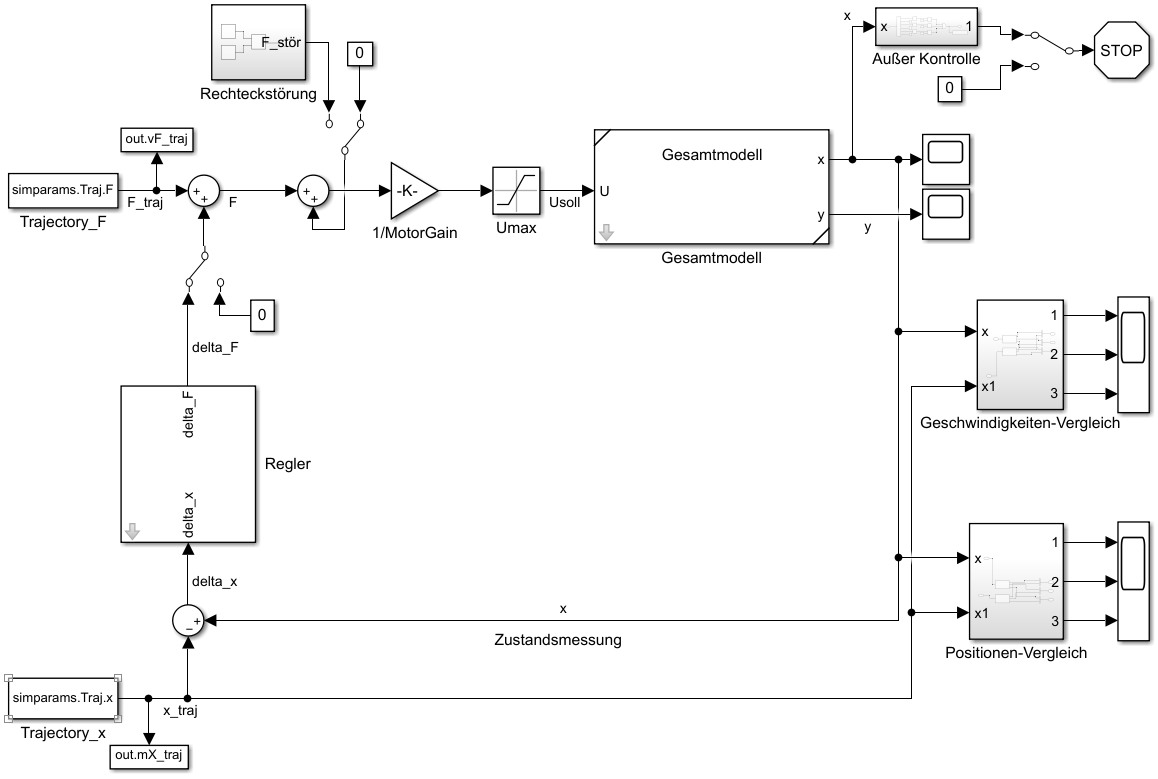
\includegraphics[width=0.98\textwidth]{Bilder/Simulink/TFR.PNG}
	\caption{Trajektorienfolgeregelung in Simulink}
	\label{fig:TFR_Simulink}
\end{figure}

Die Trajektorien werden der Simulation als \texttt{timeseries} mithilfe von \texttt{FromWorkspace} Blöcken zugeführt. Für die anschließende Auswertung in \Matlab\ hingegen können benötigte Signale über \texttt{ToWorkspace} an \Matlab\ gereicht werden. Um instabiles Verhalten zu erkennen und vorzeitig zu beenden, wird das Subsystem \texttt{AußerKontrolle} implementiert. Optional kann die Regelung zu Vergleichszwecken abgeschaltet werden. Ebenso kann kurzzeitig eine Rechteckstörung aufgeschaltet werden. Die genannten Optionen lassen sich über \texttt{ManualSwitches} ein- und ausschalten, wobei deren Zustand aus \Matlab\ heraus über die Funktion \texttt{set\_param} angesteuert werden kann.



%\section{Weitere Funktionen in \Matlab}
%...
%








\section{Stabilisierung der berechneten Trajektorien}\label{stabiltrj}

\newcommand{\scaleyplots}{0.6}

Für die mittels NMPC berechneten Trajektorien soll gezeigt werden, dass eine Stabilisierung in der Simulation mit Hilfe eines Trajektorienfolgereglers möglich ist. Im Rahmen der Vorgängerarbeit Fauvé \cite{fauve} war es nicht gelungen, die berechneten Trajektorien am störungsfreien System durch einen zeitvarianten Regler zu stabilisieren. Um das System zu stabilisieren, waren die Gewichtungsmatrizen \mat{Q} und $R$ für die Berechnung des Reglers variiert worden.

Aus diesem Grund wird ein anderer Ansatz gewählt, um eine Stabilisierung der mittels NMPC berechneten Trajektorien zu erreichen. Aus dem Skript \cite{modsim} zur Vorlesung \emph{Modellbildung und Simulation} ist bekannt, dass die Stabilität der Simulation maßgeblich von der Schrittweite und dem Integrationsverfahren abhängt. Bezüglich der Trajektorien können diese an zwei Stellen variiert werden: Einerseits innerhalb der NMPC zur Berechnung der Trajektorie und andererseits in der Simulation in \Simulink. Lässt sich eine Trajektorie mit verschiedenen Integrationsverfahren stabil simulieren, wird davon ausgegangen, dass das (ideale) System stabil ist. Über die Integration innerhalb der NMPC soll hingegen die Güte der berechneten Trajektorie variiert werden.


\subsection{Vorgehen}

Im Gegensatz zu den linearen Systemen können für nichtlineare Systeme nicht ohne Weiteres Stabilitätsgebiete für die verschiedenen Simulationsverfahren angegeben werden. Daher sind prinzipiell nur heuristische Ansätze anwendbar, um eine geeignete Schrittweite zu finden. Allgemein ist bei einer kleineren Schrittweite ein geringerer Schrittfehler und somit eine höhere Güte der Trajektorie zu erwarten. Andererseits steigen Rundungsfehler und Rechenzeit an. Bezüglich der Trajektorienberechnung wirkt sich besonders die Berechnungsdauer dominant aus. Bei einer kleineren Schrittweite muss darauf geachtet werden, dass der Prädiktionshorizont, der in Abtastpunkten angegeben wird, groß genug gewählt wird. Anderenfalls wird keine gültige Lösung mehr gefunden. Bei Fauvé \cite{fauve} wurde für die Trajektorienberechnung eine Schrittweite von $T=0,01$ (in Sekunden) bei einem Prädiktionshorizont von $N=350$ verwendet. Versuche zur Findung einer geeigneten Variation zu den von Fauvé \cite{fauve} verwendeten Parametern ergeben, dass $T=0.005$ und $N=500$ einen geeigneten Kompromiss aus möglichst kleiner Schrittweite und akzeptabler Rechenzeit liefern. 

Als Integrationsverfahren zur Trajektorienberechnung wurde von Fauvé \cite{fauve} das Euler-Verfahren eingesetzt. Als Alternative wird dem Euler-Verfahren nun das Runge-Kutta-Verfahren 4. Ordnung (RK4) gegenübergestellt.

Als weiterer Einflussfaktor auf die Güte der Trajektorien und somit auch auf ihre Stabilisierbarkeit werden die Systemparameter vermutet. Ihr Einfluss auf die Trajektorienberechnung wird in \secref{sec:trjparamtest} näher untersucht. Hierbei soll die Variation einzelner Systemparameter von einem Anfangs-Parametersatz ausgehen, für den sich die definierte Vergleichstrajektorie finden und stabilisieren lässt. Daher wird neben Schrittweite und Integrationsverfahren auch zwischen den in \secref{subsec:spdparams} definierten Parametersätzen \textit{Apprich} und \textit{Ribeiro} unterschieden.

Die Versuche zur Stabilisierbarkeit werden störungsfrei und unter Vernachlässigung der Coulomb-Reibung durchgeführt. Auf das Verhalten unter Berücksichtigung der Reibwerte wird in \secref{sec:trjparamtest} eingegangen. 

Um eine Vergleichbarkeit zur Vorgängerarbeit herzustellen, werden die Versuche sowohl mit als auch ohne Berücksichtigung der Gegeninduktion des Motormodells durchgeführt. 

Die Skripte \texttt{TFRSim\_SchlittenPendel\_run} und \texttt{TFRSim\_Gesamtmodell\_run} werden zur Durchführung der Simulationen implementiert. Beide Funktionen führen automatisiert drei Simulationen mit den Solvern \texttt{ode1} (Euler), \texttt{ode4} (RK4) und \texttt{ode45} (RK5(4) von Dormand-Prince) für eine mit \texttt{InitTrajReg} geladene Trajektorie durch. Darüber hinaus werden Plots und Animationen der Simulationsergebnisse erstellt. 
Bei den verwendeten Simulationsverfahren handelt es sich um explizite Einschrittverfahren. Der \texttt{ode4}-Solver (4. Ordnung) unterscheidet sich von \texttt{ode1} (1. Ordnung) im Wesentlichen durch die höhere Verfahrensordnung, wobei beide Verfahren mit konstanter Schrittweite operieren. Mit \texttt{ode45} wird zusätzlich ein Verfahren mit Schrittweitensteuerung eingesetzt. Hierbei handelt es sich wieder um ein Runge-Kutta-Verfahren, das jedoch gegenüber dem reinen RK4-Verfahren den Schrittfehler durch die Auswertung einer zusätzlichen Stützstelle schätzt und daraus für jeden Schritt eine eigene Schrittweite bestimmt.

Die Trajektorien werden für die Dauer des Prädiktionshorizonts und mit der gleichen Schrittweite, wie bei ihrer Berechnung verwendet wurde, simuliert. Ausnahme stellt \texttt{ode45} aufgrund der variablen Schrittweite da.

Die Funktion \texttt{TFRSim\_SchlittenPendel\_run} ruft das Simulinkmodell \texttt{TFR\_SchlittenPendel\_test} auf, das die Trajektorie direkt am Schlittenpendel-System simuliert, während \texttt{TFRSim\_Gesamtmodell\_run} das Simulinkmodell \texttt{TFR\_Gesamtmodell\_test} aufruft, das die Trajektorie am Gesamtsystem einschließlich des modellierten Gegeninduktionseffekts simuliert. Zum Vergleich werden die Trajektorien jeweils auch ohne Regler simuliert. Da die Simulationen störungsfrei sind, wird zunächst erwartet, dass auch eine Steuerung bereits gute Ergebnisse liefert.

Für die Berechnung des Reglers wurden im Voraus verschiedene QR-Matrizen als Ausgangskonfiguration getestet und sich schließlich für 
\[ 
	\mat{Q} = 
	\begin{bmatrix}
		1 & 0 & 0 & 0 & 0 & 0 \\
		0 & 1 & 0 & 0 & 0 & 0 \\
		0 & 0 & 1 & 0 & 0 & 0 \\
		0 & 0 & 0 & 1 & 0 & 0 \\
		0 & 0 & 0 & 0 & 1 & 0 \\
		0 & 0 & 0 & 0 & 0 & 1 \\
	\end{bmatrix} \ , \quad
	R = 0,1 \\
\]

entschieden, die der Arbeit von Chang \cite{chang} entnommen werden.


   

\subsection{Vergleichstrajektorie}\label{subsec:vglTrj}

Für die Versuche zur Stabilisierbarkeit und zum Einfluss der Systemparameter auf die Trajektorienberechnung (\secref{sec:trjparamtest}) wird eine Vergleichstrajektorie definiert.

Allgemein wird hierfür die klassische Aufschwungtrajektrie von AP1 nach AP4 gewählt. Es sind jedoch die in \secref{subsec:calctrj} vorgestellten Variationen zu beachten. Daher wird im Speziellen die Trajektorie 
\texttt{Traj14\_dev0\_-3.14\_-3.14\_x0max0.8} 
als Vergleichstrajektorie definiert. 
Anfangs- und Endzustand sind somit definiert als
\begin{align*}
	\vex_{\mrm{init}} =
	\begin{bmatrix}
		0 \\ 0 \\ -\pi \\ 0 \\ -\pi \\ 0
	\end{bmatrix}	, \qquad
	\vex_{\mrm{end}} =
	\begin{bmatrix}
		0 \\ 0 \\ 0 \\ 0 \\ 0 \\ 0
	\end{bmatrix} ,
\end{align*}


wobei die Positionsbeschränkung $-0,8 \leq x_0 \leq 0,8$ \ als Nebenbedingung fest vorgegeben wird.

Eine maximale Stellkraft wird in Abhängigkeit der Versuche zur Vergleichstrajektorie ergänzt.




\subsection{Ohne Gegeninduktion}\label{subsec:ohneInd}

Das System wird zunächst ohne die Gegeninduktion des Motormodells betrachtet, um im ersten Schritt an den Stand von Fauvé \cite{fauve} anzuknüpfen. Entsprechend wird auch die Stellkraftbegrenzung auf die in Fauvé \cite{fauve} verwendete Maximalkraft $F_{\mrm{max}}=\valunit{400}{N}$ eingestellt. 

Die Ergebnisse für $T=0.01$ und $N=350$ sind in \tabref{tab:T001N350Fmax400} zusammengefasst.
\begin{table}[h]
	\centering
	\caption{$T=0.01, \ N=350$}
		\begin{tabular}{c|c|c|c|c|c}
			\rowcolor[gray]{0.9}
			\multicolumn{2}{c|}{\textbf{Simulation}} & \multicolumn{2}{c|}{\textbf{Apprich}} & \multicolumn{2}{c}{\textbf{Ribeiro}} \\
			\midrule
			\rowcolor[gray]{0.9}
			\textbf{Solver} & \textbf{TFR} & \textbf{Euler} & \textbf{RK4} & \textbf{Euler} & \textbf{RK4} \\
			\midrule
			\cellcolor[gray]{0.9}  											& \cellcolor[gray]{.9}ohne & "`leicht instabil"' & instabil       & instabil & instabil\\
			\multirow{-2}{*}{\cellcolor[gray]{.9}ode1}	& \cellcolor[gray]{.9}mit  & \textbf{stabil} & \textbf{stabil} & instabil & "`leicht instabil"'\\
			\midrule
			\cellcolor[gray]{0.9}  											& \cellcolor[gray]{.9}ohne    & instabil	&  instabil & instabil & instabil\\
			\multirow{-2}{*}{\cellcolor[gray]{.9}ode4}	& \cellcolor[gray]{.9}mit     & instabil  & instabil  & instabil & \textbf{stabil}\\
			\midrule	
			\cellcolor[gray]{0.9}  											& \cellcolor[gray]{.9}ohne    & instabil &  instabil    & instabil 	& instabil\\
			\multirow{-2}{*}{\cellcolor[gray]{.9}ode45}	& \cellcolor[gray]{.9}mit     & instabil &  instabil    & instabil 	& "`leicht instabil"'\																							
		\end{tabular}
	\label{tab:T001N350Fmax400}
\end{table}

Es wird zwischen 

%\begin{center}
	%\begin{tabular}{cl}
		%stabil & Aufschwung gelingt, AP4 kann bis zum Ende der Simulation gehalten werden \\
		%"`leicht instabil"' & Aufschwung gelingt weitgehend, AP4 wird nicht gehalten  \\
		%instabil & Aufschwung gelingt nicht \\
	%\end{tabular}
%\end{center}
\begin{itemize}
	\item \emph{stabil} - Aufschwung gelingt, AP4 kann bis zum Ende der Simulation gehalten werden
	\item \emph{"`leicht instabil"'} - Aufschwung gelingt weitgehend, AP4 wird nicht gehalten
	\item \emph{instabil} - Aufschwung gelingt nicht
\end{itemize}
unterschieden. Zum besseren Verständnis soll die Zuordnung der dargestellten Ergebnisse an Hand repräsentativer Beispiele erläutert werden.

Zunächst wird der Eintrag links oben in \tabref{tab:T001N350Fmax400} betrachtet. Hierbei wird die Vergleichstrajektorie mit dem Apprich-Parametersatz und dem Euler-Verfahren berechnet und anschließend auch wieder mit dem Euler-Verfahren am Schlittendoppelpendel simuliert. Die in \figref{fig:F400T0.01_app_euler_ode1} dargestellten Ergebnisse zeigen die Verläufe der Ausgänge und der Stellkraft für das zunächst ungeregelte System. Es ist zu erkennen, dass der Aufschwung ohne Regelung gelingt, AP4 jedoch nicht gehalten wird. Das Ergebnis wird daher als \textit{leicht instabil} beurteilt. In der anschließenden Simulation am geregelten System kann das Pendel schließlich bis zum Ende der Simulationszeit stabilisiert werden.
\begin{figure}[h]
	\centering
		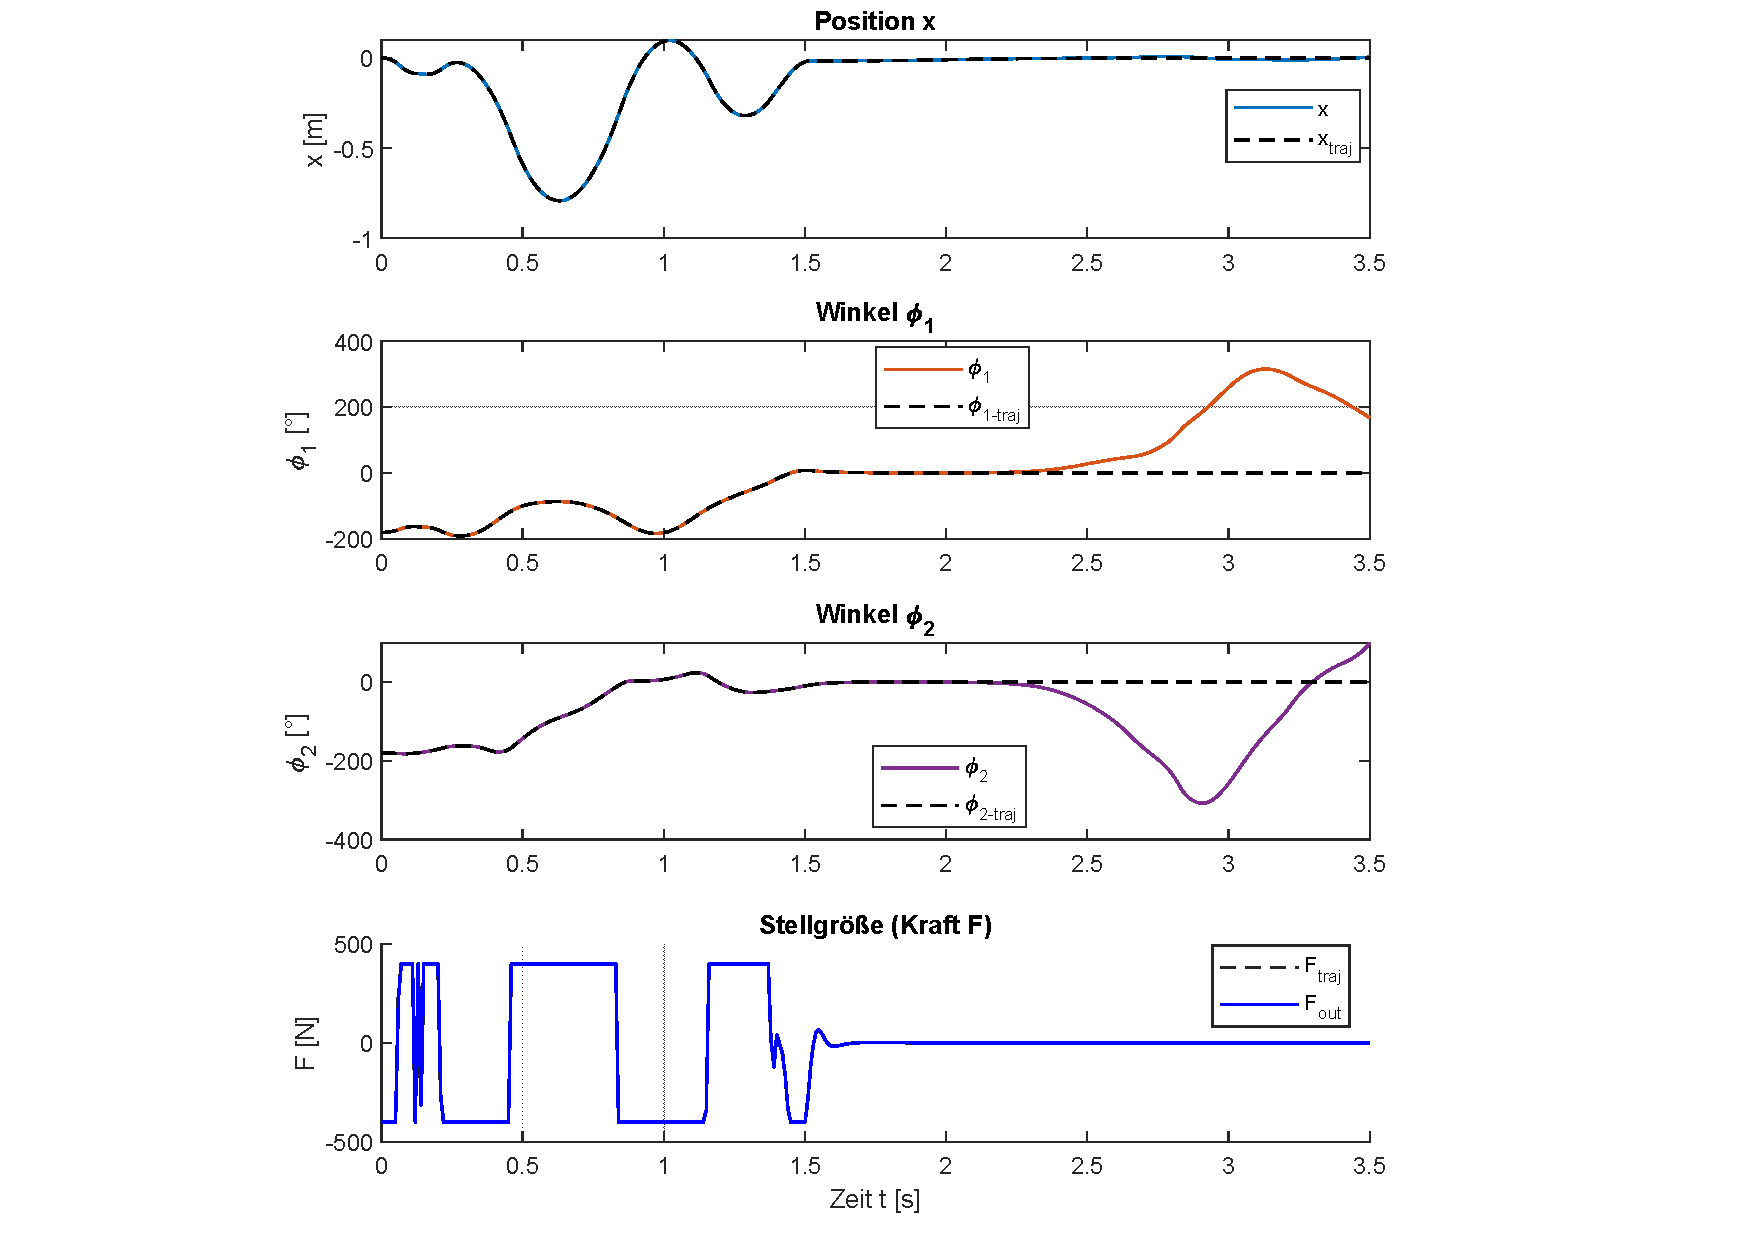
\includegraphics[scale=\scaleyplots]{Bilder/Trajektorien/F400T0.01_app_euler_ode1.pdf}
	\caption{$T=0,01$, $N=350$, Apprich-Parameter, Euler-MPC, ode1-Sim, ohne Regelung}
	\label{fig:F400T0.01_app_euler_ode1}
\end{figure}

Mit den Verfahren \texttt{ode4} und \texttt{ode45} am ungeregelten System zeigen die Verläufe demgegenüber hohe Abweichungen von der Trajektorie. Erwartungsgemäß lassen sie sich anschließend am geregelten System nicht stabilisieren. Die Verläufe werden daher als \textit{instabil} bewertet. 

Die mit dem Eulerverfahren berechnete Trajektorie lässt sich zwar stabilisieren, jedoch nur, wenn die bei der Trajektorienberechnung gemachten Schrittfehler durch das gleiche Verfahren in der Simulation näherungsweise reproduziert werden. Dass die Steuerung alleine nicht ausreicht, obwohl mit gleicher numerischer Fehlerfortpflanzung simuliert wird, lässt sich einerseits damit begründen, dass die Nebenbedingungen des Optimierungsverfahrens mit bestmöglicher, jedoch endlicher Genauigkeit eingehalten werden. Die beobachteten Genauigkeiten für die Nebenbedingungen liegen zwischen $10^{-13}$ und $10^{-34}$ für (lokal) optimale Lösungen. Andererseits ist insbesondere zu beachten, dass der zu erreichende Endwert durch die Optimierung lediglich angenähert wird. Die im Rahmen der Arbeit beobachteten absoluten Fehler einzelner Zustandsgrößen im letzten Prädiktionsschritt lagen bei den vom Optimierer ausgegebenen "`optimalen"' Lösungen im Bereich von $10^{-5}$ und $2 \cdot 10^{1}$.

Als weiteres Beispiel wird die für den Ribeiro-Parametersatz und das RK4-Verfahren berechnete Trajektorie in der Simulation mit \texttt{ode4} betrachtet. Die Verläufe sind für das ungeregelte System in \figref{fig:F400T0.01_rib_rk4_ode4} zu sehen. 
\begin{figure}[h]
	\centering
		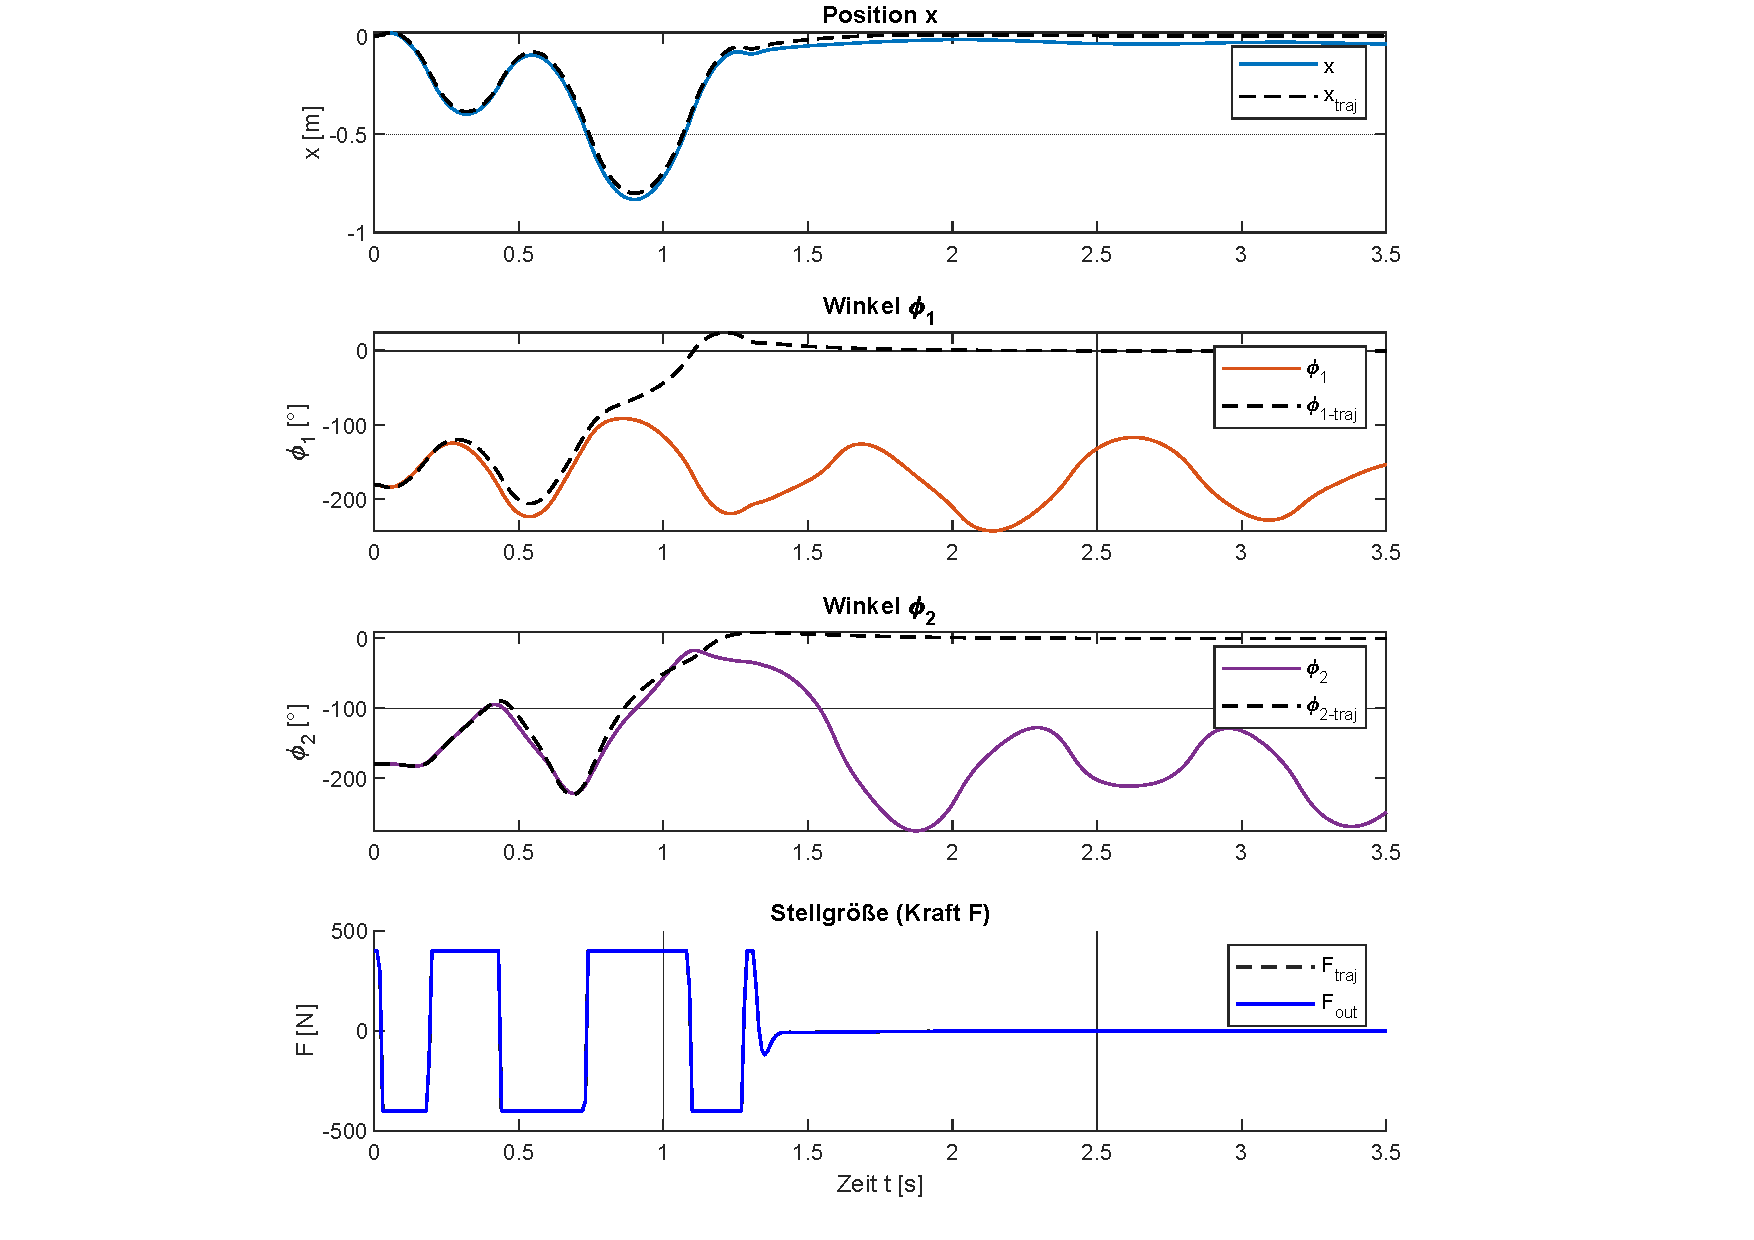
\includegraphics[scale=\scaleyplots]{Bilder/Trajektorien/F400T0.01_rib_rk4_ode4.pdf}
	\caption{$T=0,01$, $N=350$, Ribeiro-Parameter, RK4-MPC, ode4-Sim, ohne Regelung}
	\label{fig:F400T0.01_rib_rk4_ode4}
\end{figure}

Es ist deutlich ersichtlich, dass der Aufschwung nicht gelingt. Das erste Pendel fällt bereits gleich zu Anfang des Aufschwungs zurück, sodass in der Folge beide Pendel unkontrolliert zu schwingen beginnen. Die Verläufe werden daher als \textit{instabil} bewertet.
In \figref{fig:F400T0.01_rib_rk4_ode4_TFR_QR-alt} sind demgegenüber die Verläufe mit Trajektorienfolgeregelung zu sehen. 
\begin{figure}[h]
	\centering
		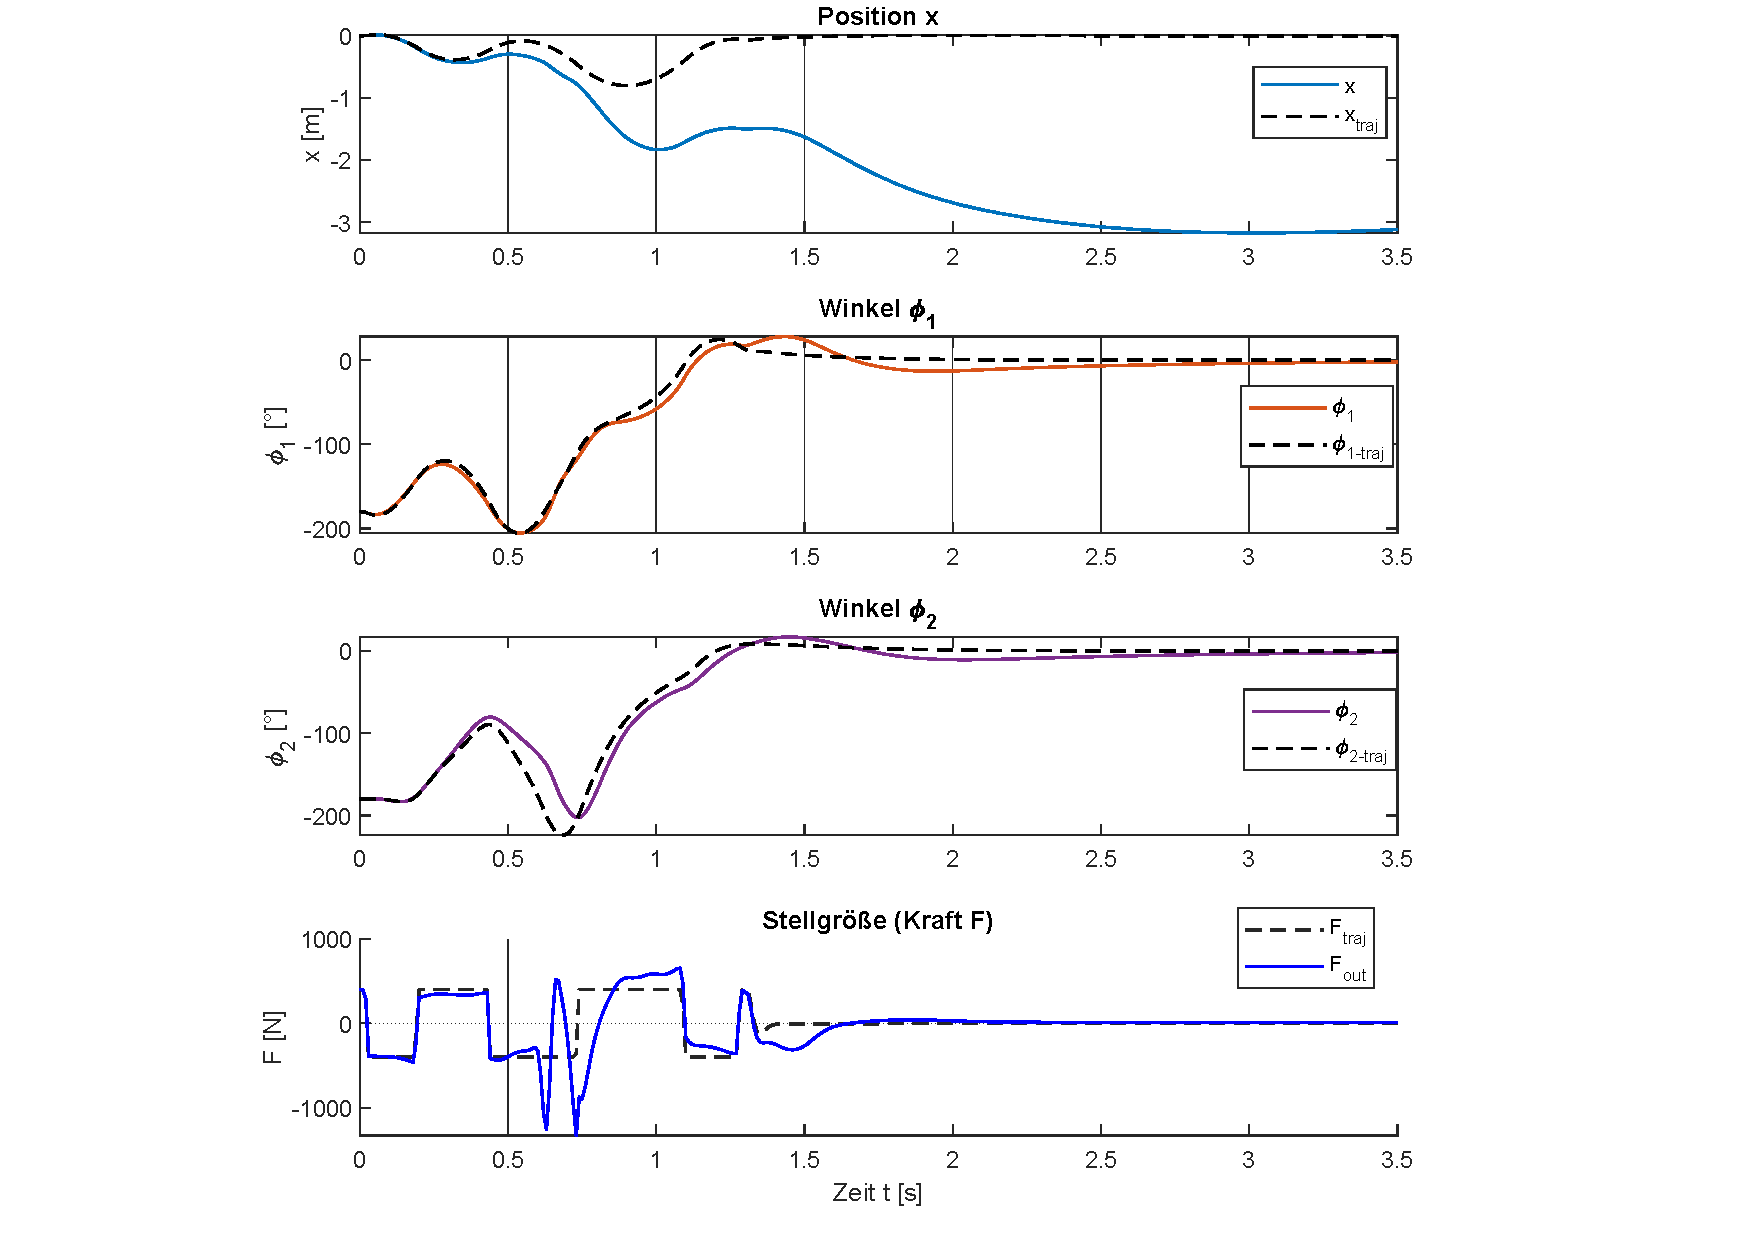
\includegraphics[scale=\scaleyplots]{Bilder/Trajektorien/F400T0.01_rib_rk4_ode4_TFR_QR-alt.pdf}
	\caption{$T=0,01$, $N=350$, Ribeiro-Parameter, RK4-MPC, ode4-Sim, mit Regelung}
	\label{fig:F400T0.01_rib_rk4_ode4_TFR_QR-alt}
\end{figure}

Das Doppelpendel kann demnach stabilisiert werden, jedoch ist in der Schlittenposition ein "`Weglaufen"' zu beobachten. Dieses sorgt dafür, dass die vorgegebene Positionsbegrenzung weit überschritten wird. Es liegt daher nahe, dass durch eine höhere Bestrafung der Position mit Hilfe der QR-Parameter des Reglers eine Verringerung der maximalen Auslenkung zu erwarten ist. Eine Variation von $Q_1$ ergibt, dass mit einer Erhöhung von $Q_1=1$ auf wahlweise $Q_1=1,05$ oder $Q_1=4,5$ sich die maximale Positionsauslenkung von etwa \valunit{-3,2}{m} auf \valunit{-2,5}{m} senken lässt. Damit liegt die erreichte Auslenkung weiterhin weit außerhalb der zulässigen Begrenzung von \valunit{\pm 0,8}{m}. Es zeigt sich außerdem, dass die Stabilisierung der betrachteten Trajektorie empfindlich auf Veränderung von $Q_1$ reagiert. Bereits bei $Q_1=1,07$ bzw. $Q_1=4,6$ wird das System instabil. Da allgemein jedoch eine Stabilisierung erreicht wird, ist die Trajektorie für die Simulation \texttt{ode4} am geregelten System als \textit{stabil} bewerten. 

Nach dem beschriebenen Vorgehen werden auch die weiteren Simulationsversuche ausgewertet. Die Ergebnisse in \tabref{tab:T001N350Fmax400} zeigen, dass sich drei der vier berechneten Trajektorien in zumindest einer der drei betrachteten Simulationen stabilisieren lässt. Die mit dem Euler-Verfahren und den Ribeiro-Parametern berechnete Trajektorie fällt dabei auf, da eine Stabilisierung generell in keiner der betrachteten Simulationen erreicht wird. Als Nächstes wird daher eine höhere Güte der Trajektorien gefordert, indem die Schrittweite für die Trajektorienberechnung halbiert wird bei entsprechender Erhöhung des Prädiktionshorizonts. Die Ergebnisse für $T=0.005$ und $N=500$ sind in \tabref{tab:T0005N500Fmax400} dargestellt.
\begin{table}[H]
	\centering
	\caption{$T=0.005, \ N=500$}
		\begin{tabular}{c|c|c|c|c|c}
			\rowcolor[gray]{0.9}
			\multicolumn{2}{c|}{\textbf{Simulation}} & \multicolumn{2}{c|}{\textbf{Apprich}} & \multicolumn{2}{c}{\textbf{Ribeiro}} \\
			\midrule
			\rowcolor[gray]{0.9}
			\textbf{Solver} & \textbf{TFR} & \textbf{Euler} & \textbf{RK4} & \textbf{Euler} & \textbf{RK4} \\
			\midrule
			\cellcolor[gray]{0.9}  											& \cellcolor[gray]{.9}ohne & "`leicht instabil"'  & "`leicht instabil"' & instabil & Trajektorie\\
			\multirow{-2}{*}{\cellcolor[gray]{.9}ode1}	& \cellcolor[gray]{.9}mit  & \textbf{stabil} & \textbf{stabil} 			& instabil 				 & 	\\
			\midrule
			\cellcolor[gray]{0.9}  											& \cellcolor[gray]{.9}ohne & instabil	& "`leicht instabil"' & instabil & nicht\\
			\multirow{-2}{*}{\cellcolor[gray]{.9}ode4}	& \cellcolor[gray]{.9}mit  & instabil & \textbf{stabil} & instabil & \\
			\midrule	
			\cellcolor[gray]{0.9}  											& \cellcolor[gray]{.9}ohne & instabil	&  "`leicht instabil"' & instabil 	& gefunden\\
			\multirow{-2}{*}{\cellcolor[gray]{.9}ode45}	& \cellcolor[gray]{.9}mit  & instabil	&  \textbf{stabil}  & instabil 	& \																											
		\end{tabular}
	\label{tab:T0005N500Fmax400}
\end{table}

Hierbei fällt auf, dass die Trajektorie, die mit Hilfe des Apprich-Parametersatzes und des RK4-Verfahrens berechnet wird, mit Hilfe des Reglers in allen drei Simulationen stabilisiert werden kann. Auch die Verläufe am ungeregelten System liefern bereits gute Ergebnisse. Die Stabilisierung durch den Regler erfolgt zudem innerhalb der vorgegebenen Positionsbegrenzung bei gleichzeitig geringer Abweichung von der Trajektorie.




\subsection{Mit Gegeninduktion}\label{subsec:mitInd}

Wird die Gegeninduktion des Motors berücksichtigt und am Gesamtmodell simuliert, fällt zunächst auf, dass mit $F_{\mrm{max}}= \valunit{400}{N}$ für den konstanten Bereich der Strombegrenzung keine der vier untersuchten Trajektorien gefunden wird. Durch eine Variation der Maximalkraftbegrenzung ergibt sich $F_{\mrm{max}}= \valunit{410}{N}$ als neue Grenze. Damit ist weiterhin eine Stellgrößenreserve von \valunit{11}{N} gegenüber der zuletzt am Versuchsstand eingestellten Maximalkraft von $F_{\mrm{max}}= \valunit{421}{N}$ gewährleistet. 

Für $T=0.01$ und $N=350$ kann dennoch keine der Trajektorien gefunden werden. Die Ergebnisse für $T=0.005$ und $N=500$ sind in \tabref{tab:T001N350Fmax410} zusammengetragen. Die Trajektorie auf Basis der Apprich-Parameter und des RK4-Verfahrens bestätigt die Ergebnisse aus \secref{subsec:ohneInd}. Sie lässt sich unabhängig vom betrachteten Simulationsverfahren stabilisieren.
\begin{table}[H]
	\centering
	\caption{$T=0.005, \ N=500$}
		\begin{tabular}{c|c|c|c|c|c}
			\rowcolor[gray]{0.9}
			\multicolumn{2}{c|}{\textbf{Simulation}} & \multicolumn{2}{c|}{\textbf{Apprich}} & \multicolumn{2}{c}{\textbf{Ribeiro}} \\
			\midrule
			\rowcolor[gray]{0.9}
			\textbf{Solver} & \textbf{TFR} & \textbf{Euler} & \textbf{RK4} & \textbf{Euler} & \textbf{RK4} \\
			\midrule
			\cellcolor[gray]{0.9}  											& \cellcolor[gray]{.9}ohne & Trajektorie  & instabil & leicht instabil & Trajektorie\\
			\multirow{-2}{*}{\cellcolor[gray]{.9}ode1}	& \cellcolor[gray]{.9}mit  &   						& \textbf{stabil} & \textbf{stabil} 				 & 	\\
			\midrule		
			\cellcolor[gray]{0.9}  											& \cellcolor[gray]{.9}ohne & nicht	& instabil 						& instabil & nicht\\
			\multirow{-2}{*}{\cellcolor[gray]{.9}ode4}	& \cellcolor[gray]{.9}mit  &        & \textbf{stabil}   	& instabil & \\
			\midrule	
			\cellcolor[gray]{0.9}  											& \cellcolor[gray]{.9}ohne & gefunden 	&  instabil    			& instabil 	& gefunden\\
			\multirow{-2}{*}{\cellcolor[gray]{.9}ode45}	& \cellcolor[gray]{.9}mit  &  					&  \textbf{stabil}  & instabil 	& \\																											
		\end{tabular}
	\label{tab:T001N350Fmax410}
\end{table}

Durch Variation der QR-Parameter können die Simulationsergebnisse zudem noch optimiert werden. Sehr gute Ergebnisse werden für die QR-Matrizen in \tabref{tab:NeueQR} erzielt.
\begin{table}[h]
	\centering
	\caption{Neue QR-Matrizen für Apprich-RK4-Trajektorie}
		\begin{tabular}{cll}
			\toprule
			ode1        & $\mat{Q} = \mrm{diag}\left(1, 1, 100, 1, 100, 1\right)$           & $R=0,01$ \\
			ode4, ode45 & $\mat{Q} = \mrm{diag}\left(1000, 0.01, 100, 0.1, 100, 0.1\right)$ & $R=0,001$ \\
			\bottomrule
		\end{tabular}
	\label{tab:NeueQR}
\end{table}

Die Ausgangsverläufe für die Simulation mit \texttt{ode45} und den neuen QR-Parametern sind in \figref{fig:F410T0.005_app_rk4_ode45_TFR_QR-neu} dargestellt. Im Vergleich zu den Plots in \secref{subsec:ohneInd} wird im Stellgrößenverlauf zusätzlich zwischen $F_\mrm{in}$ und $F_\mrm{out}$ unterschieden. $F_\mrm{in}$ bezeichnet den durch Regler und Trajektorie festgelegten Stellwert, der auf das Gesamtsystem gegeben wird. Auf Grund der Strombegrenzungskennlinie (vgl. \figref{fig:Stromkennlinie}) kann am Ausgang des Motors jedoch ein abweichender Kraftverlauf entstehen, der mit $F_\mrm{out}$ dargestellt wird. Da die Stromkennlinie in den Nebenbedingungen der Trajektorienberechnung berücksichtigt wird, entstehen Abweichungen zwischen $F_\mrm{in}$ und $F_\mrm{out}$ in erster Linie auf Grund des Reglers. 
\begin{figure}[h]
	\centering
		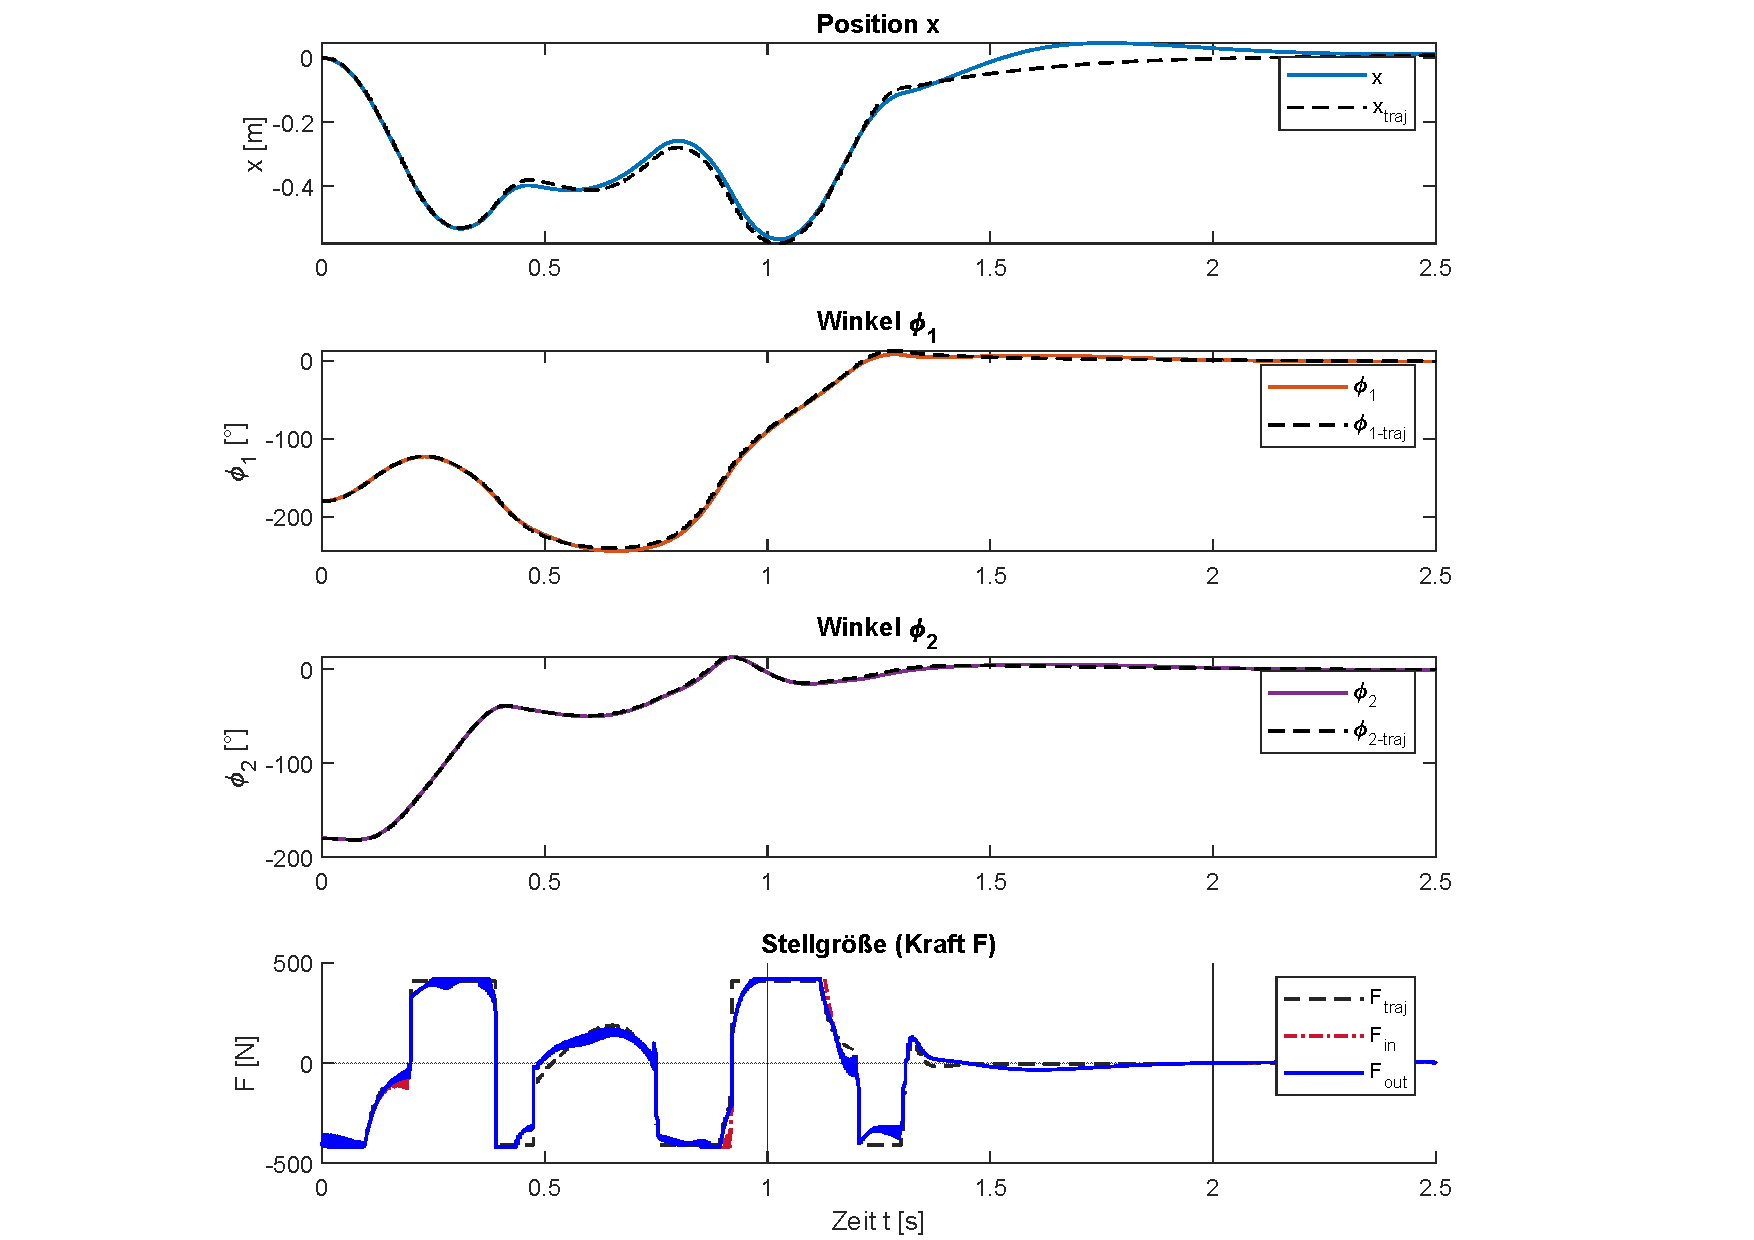
\includegraphics[scale=\scaleyplots]{Bilder/Trajektorien/F410T0.005_app_rk4_ode45_TFR_QR-neu.pdf}
	\caption{$T=0,005$, $N=500$, Apprich-Parameter, RK4-MPC, ode45-Sim, mit Regelung}
	\label{fig:F410T0.005_app_rk4_ode45_TFR_QR-neu}
\end{figure}

\textbf{Fazit:}
Es lässt sich zeigen, dass die mit dem Verfahren der NMPC berechneten Trajektorien in der Simulation stabilisierbar sind. Zudem bestätigt sich die Vermutung, dass die Schrittweite und die Wahl des Integrationsverfahrens zur Berechnung der Trajektorien einen Einfluss auf die numerische Stabilität haben. Eine geringere Schrittweite und ein Integrationsverfahren mit geringerem Schrittfehler haben in den betrachteten Versuchsdurchführungen zu einer höheren Stabilität geführt. Darüber hinaus fällt auf, dass die Apprich-Parameter gegenüber den Ribeiro-Parametern ein günstigeres Verhalten aufweisen. Der Einfluss der Modellparameter wird im folgenden Kapitel daher näher untersucht. 






\section{Untersuchung des Einflusses der Modellparameter}\label{sec:trjparamtest}

Im Folgenden soll der Einfluss der Modellparameter auf die Trajektorienberechnung untersucht werden.

\subsection{Vorgehen}

Gegenstand der Untersuchung sind die Parameter Masse, Massenträgheitsmoment und Schwerpunkt jedes Pendelstabs. Durch Variation der Parameter sollen günstige Wertebereiche identifiziert und formuliert werden, in denen gültige Trajektorien gefunden werden können. Darüber hinaus werden die Variationsergebnisse in Bezug auf Häufung und Güte der gültigen Trajektorien analysiert.

Die Parameterwerte für die Parameteruntersuchung orientieren sich an den Werten der zum Versuchsstand aufgestellten Parametersätze aus \secref{subsec:spdparams}. Die Schrittweiten der Parametervariationen werden möglichst gering gewählt, um die Aussagekraft der Ergebnisse durch eine hohe Auflösung sicherzustellen. Auf Grund der hohen Berechnungszeiten für die Trajektorien, sind beliebig kleine Schrittweiten jedoch nicht möglich, sodass ein sinnvoller Kompromiss zwischen Auflösung und Berechnungszeit gefunden werden muss. Das geplante Variationsvorhaben ist in \tabref{tab:Parametervariationen} aufgeführt. Hierbei wird die konstruktive Realisierbarkeit der Parameterwerte nicht berücksichtigt, da vorwiegend der Einfluss der Modellparameter auf die Berechnungsergebnisse untersucht wird.
\begin{table}[h]
	\centering
	\caption{Parametervariationen}
		\begin{tabular}{lllll}
	    \toprule
			Parameter & Startwert & Endwert & Schrittweite & Anzahl Trajektorien \\
			\midrule
			$m_1 \ [\unit{kg}]$     & $0$ & $2$    & $0,01$   & $201$ \\
			$m_2 \ [\unit{kg}]$     & $0$ & $2$    & $0,01$   & $201$ \\
			$J_1 \ [\unit{kgm^2}]$  & $0$ & $0,02$ & $0,0001$ & $201$ \\
			$J_2 \ [\unit{kgm^2}]$  & $0$ & $0,02$ & $0,0001$ & $201$ \\
		  $s_1 \ [\unit{m}]$      & $0$ & $0,29$ & $0,001$  & $291$ \\
			$s_2 \ [\unit{m}]$      & $0$ & $0,338$& $0,001$  & $339$ \\
			\bottomrule
		\end{tabular}
	\label{tab:Parametervariationen}
\end{table}

Die zu untersuchenden Modellparameter werden einzeln gegenüber einem definierten Ausgangsparametersatz variiert, wobei alle weiteren Parameter konstant gehalten werden. Zur Durchführung der Versuche wird die Funktion \texttt{examParameters} implementiert. Ihr kann eine Versuchsreihe bestehend aus der Bezeichnung des zu untersuchenden Parameters und einem Vektor mit den Variationswerten übergeben werden. Über den Aufruf der in \secref{subsec:searchtrj} beschriebenen Funktion \texttt{searchTrajectories} werden damit die benötigten Trajektorienberechnungen ausgeführt. Die Trajektorien werden anschließend im Ordner \texttt{ParameterExams} gespeichert. Um die Ergebnisse später sinnvoll identifizieren zu können, wird der in \secref{subsec:searchtrj} definierten Namenskonvention eine Endung bestehend aus der Bezeichnung des untersuchten Parameters und dessen Wert angefügt. 

Zur Bewertung der betrachteten Parametervariationen wird zunächst unterschieden, ob für die jeweilige Variation eine Trajektorie gefunden werden kann oder nicht. Darüber hinaus wird das Gütemaß $J_\mrm{dev}$ eingeführt, um die Güte der gefundenen Lösungen zu quantifizieren. Der Ansatz für das Gütemaß basiert auf der Definition von Trajektorien durch ihre Randbedingungen. Da diese bei der Optimierung mit endlicher Genauigkeit erfüllt werden (\vgl \secref{subsec:ohneInd}), ist der resultierende Fehler ein Kriterium für die Güte der Trajektorien.

Das Gütemaß wird mit
	\[
	J_\mrm{dev} = \left\| \Delta \ve{x_{\mrm{init}}} \right\| + \left\| \Delta \ve{x_{\mrm{end}}} \right\|
	\]
	
definiert. $\left\|\Delta \ve{x_\mrm{init}}\right\|$ und $\left\|\Delta \ve{x_\mrm{end}}\right\|$ sind hierbei als die euklidischen Normen der mit den Fehlerdifferenzen gefüllten Zustandsvektoren in Anfangs- und Endlage der Trajektorie zu verstehen.
\[
	\left\| \Delta \ve{x_{\mrm{init}}} \right\| = \sqrt{ \sum_{i=1}^6 \left( x_{\mrm{Traj,}i}(t_\mrm{init}) - x_{\mrm{init,}i} \right)^2 }
\]

mit $t_\mrm{init} = 0$ und
	\[
	\left\| \Delta \ve{x_{\mrm{end}}} \right\| = \sqrt{ \sum_{i=1}^6 \left( x_{\mrm{Traj,}i}(t_{\mrm{end}}) - x_{\mrm{end,}i} \right)^2 }
\]

mit $t_{\mrm{end}} = (N+1) \cdot T$

Wie in \secref{stabiltrj} erläutert, ist im Falle eine konvergierten Lösung nur der Endwertfehler relevant, da dieser indirekt durch die Zielfunktion und nicht durch die Nebenbedingungen für die Optimierung vorgegeben wird. Unter der Voraussetzung einer konvergierten Lösung gilt daher
\[
	J_\mrm{dev} = \left\| \Delta \ve{x_{\mrm{end}}} \right\| \ .
	\]	 

Basierend auf den Erkenntnissen des vorherigen Abschnitts wird weiterhin folgende Ausgangskonfiguration für die Berechnung der Trajektorien gewählt, wobei die Gegeninduktion des Motors berücksichtigt und die Coulomb-Reibung vernachlässigt wird:
\begin{itemize}
	\item $T = 0,005$
	\item $N = 500$
	\item RK4-Integration
	\item Apprich-Parameter
\end{itemize}

Als Trajektorie wird die in \secref{subsec:vglTrj} definierte Vergleichstrajektorie verwendet. Die Gewichtungsmatrizen für die Zielfunktion sind \secref{subsec:calctrj} zu entnehmen.






\subsection{Durchführung und Ergebnisse}\label{subsec:trjParTestRes}

Die Auswertung erfolgt mit Hilfe der Funktion \texttt{plot\_Jdev\_params}. Mit dieser wird das Gütemaß berechnet und über dem untersuchten Parameter in einem Koordinatensystem aufgetragen. Hierbei werden auch die berechneten Werte des Apprich- und des Ribeiro-Parametersatzes nach \secref{subsec:spdparams} als Vergleichswerte durch die Funktion hinzugefügt. Es ist zu beachten, dass der eingefügte Ribeiro-Vergleichswert sich nur auf den untersuchten Parameter bezieht. Die übrigen Parameter werden weiterhin dem Apprich-Parametersatz entnommen. Liegen die Werte von Apprich und Ribeiro nicht auf einem durch \tabref{tab:Parametervariationen} definierten Variationswert, ist eine Erhöhung der Anzahl an berechneten Trajektorien zu berücksichtigen. Trajektorien ohne lokale Konvergenz zu einem Optimum werden als ungültig gewertet.

Werden zunächst die relativen Häufigkeiten gültiger Trajektorien $\hg$ miteinander verglichen, zeigt sich, dass neben dem Massenträgheitsmoment von Stab 1 besonders die Variation der beiden Stabmassen einen vergleichsweise geringen Anteil an Trajektorien verzeichnet, bei denen der Optimierer lokal konvergiert \bzw eine gültige Lösung findet (\tabref{tab:statTrj}). Der Einfluss von $m_1$ und $m_2$ sowie $J_1$ auf die Trajektorienberechnung ist daher als hoch anzusehen. 

\begin{table}[h]
	\centering
	\caption{Statistik gültiger Trajektorien}
		\begin{tabular}{lllll}
			\toprule
			Parameter  & Ungültig & Gültig & Gesamt & Gültigkeitsanteil \hg \\
			\midrule
			$m_1 \ [\unit{kg}]$     & $177$ & $26$    & $203$   & $13 \% $ \\
			$m_2 \ [\unit{kg}]$     & $189$ & $14$    & $203$   & $7 \% $ \\
			$J_1 \ [\unit{kg m^2}]$  & $175$ & $28$    & $203$   & $14 \%$ \\
			$J_2 \ [\unit{kg m^2}]$  & $79$  & $124$   & $203$   & $61 \%$ \\
			$s_1 \ [\unit{m}]$      &  $231$  & $62$ & $293$  &  $21 \%$\\
			$s_2 \ [\unit{m}]$      & $190$ & $150$   & $340$  & $44 \%$ \\
			\bottomrule
		\end{tabular}
	\label{tab:statTrj}
\end{table}

Besonders auffällig ist in diesem Zusammenhang $m_2$ mit einem Anteil gültiger Trajektorien von nur $\hg=7\%$. \figref{fig:trjvarm2} visualisiert die Ergebnisse der $m_2$-Variation. Die Datenpunkte für Apprich und Ribeiro werden allgemein durch Quadrate markiert, wobei Dunkelblau für Apprich und Dunkelorange für Ribeiro steht. Da für die Ribeiro-Masse in diesem Fall keine gültige Trajektorie gefunden wird, erscheint der Wert als "`x"'-Markierung auf der Abszisse. Die übrigen ungültigen Trajektorien sind hingegen im Sinne der Übersichtlichkeit nicht explizit dargestellt.

\begin{figure}
	\centering
		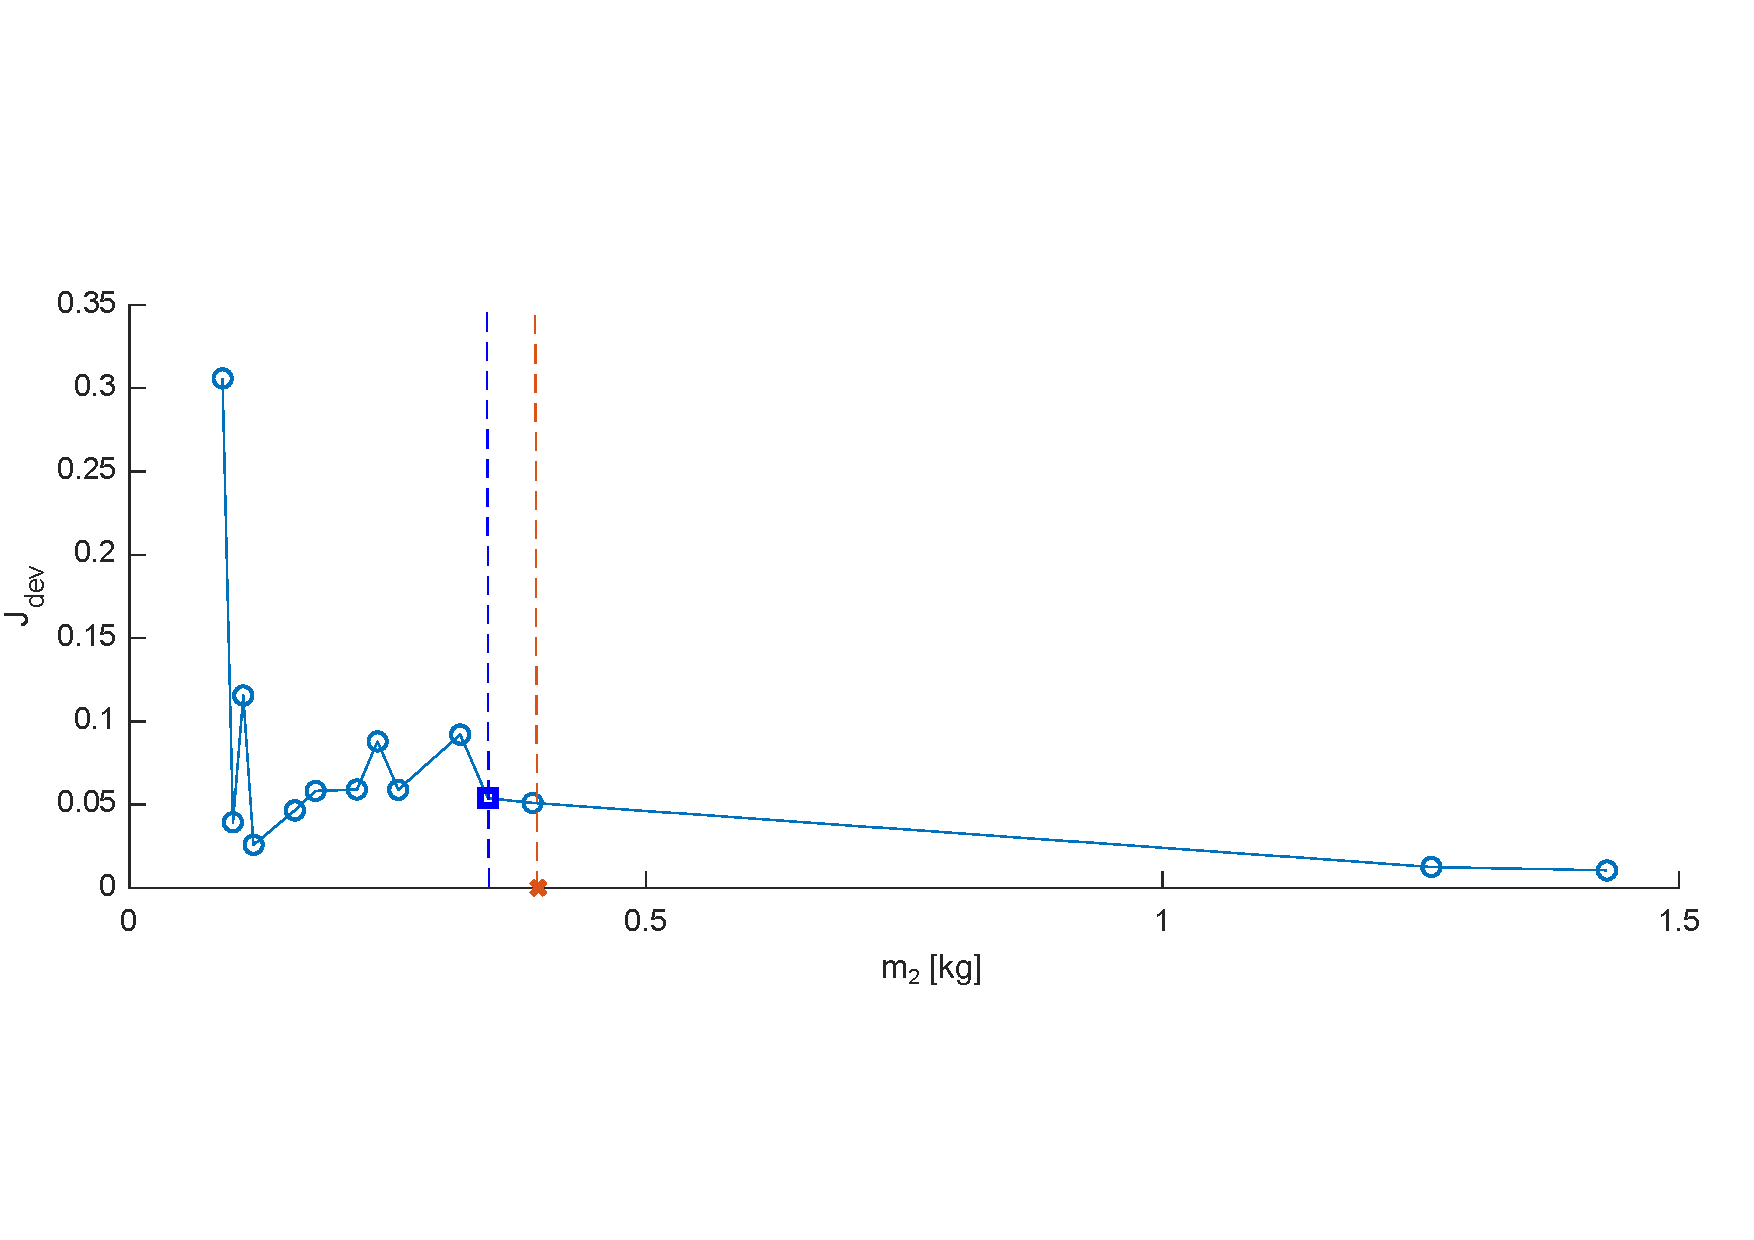
\includegraphics[width=0.8\textwidth]{Bilder/Trajektorien/m2.pdf}
	\caption{Variation $m_2$}
	\label{fig:trjvarm2}
\end{figure}

In der Abbildung zu erkennen ist, dass 12 von 14 gefundenen Trajektorien im Bereich $\valunit{0,09}{kg}\leq m_2 \leq\valunit{0,39}{kg}$ liegen. Zwei weitere Trajektorien werden gefunden, wenn der Wertebereich bis \valunit{1,43}{kg} deutlich vergrößert wird. Eine Erweiterung bis \valunit{2}{kg} führt schließlich zu keiner weiteren Trajektorie mehr. Wird nur der Bereich $\valunit{0,09}{kg}\leq m_2 \leq\valunit{0,39}{kg}$ betrachtet, steigt die Häufigkeit gültiger Trajektorien von $\hg=7\%$ auf $\hg=38\%$. Es treten jedoch weiterhin auch ungültige Lösungen auf. Zwischen den diskret untersuchten Parametern (vgl. \tabref{tab:Parametervariationen}) existieren im Kontinuierlichen unendlich viele weitere, potentielle Parameterwerte, für die eine Trajektorie berechnet werden kann. Wird die relative Häufigkeit gültiger Trajektorien $\hg$ als Konvergenz-Wahrscheinlichkeit  $\hg\approx\Pkon$ der Optimierung interpretiert, dann kann auch eine Aussage über die weiteren, potentiellen Trajektorien im Kontinuierlichen innerhalb des betrachteten Bereichs getroffen werden. Der Bereich $\valunit{0,09}{kg}\leq m_2 \leq\valunit{0,39}{kg}$ signalisiert somit allgemein eine hohe Konvergenzwahrscheinlichkeit $\Pkon$. Der markierte Apprich-Wert für $m_2$ befindet sich bereits nahe der Grenze dieses Bereichs, der Ribeiro-Wert sogar leicht darüber. Im Sinne einer hohen Konvergenzwahrscheinlichkeit kommt daher nur eine Verringerung von $m_2$ in Frage. 

Bei Betrachtung der Güte der gefundenen Trajektorien, fällt auf, dass für 12 von 14 Trajaktorien $J_\mrm{dev} = \left\| \Delta \ve{x_{\mrm{end}}} \right\|<0,1$ gilt. Besonders gut wird der Endwert für die beiden Trajektorien approximiert, die jedoch außerhalb des Bereichs von $\Pkon\approx38\%$ liegen und daher als "`Ausreißer"' bezeichnet werden. Die ungünstigeren Werte mit  $J_\mrm{dev}<0,1$ liegen hingegen im unteren Grenzbereich. Die Erfahrung in der Simulation hat gezeigt, dass für $J_\mrm{dev}\gg1$ ohne Weiteres keine QR-Matrizen für die Regelung gefunden werden, mit denen die Trajektorien stabilisiert werden können. Diese Trajektorien werden daher in Bezug auf Stabilisierbarkeit als ungünstig bis unbrauchbar eingeschätzt. Damit liegen die gefundenen Trajektorien mit $J_\mrm{dev}<1$ im akzeptablen Bereich. Ein eindeutiges Muster bezüglich der Trajektoriengüte lässt sich in \figref{fig:trjvarm2} jedoch nicht erkennen.

Für $m_2$ wird schließlich der Bereich $\valunit{0,09}{kg}\leq m_2 \leq\valunit{0,39}{kg}$ mit einer Konvergenzwahrscheinlichkeit von $\Pkon\approx\hg=38 \%$ als Wertebereich gültiger Trajektorien formuliert, wobei die zwei identifizierten "`Ausreißer"' vernachlässigt werden. Für den aktuelle Ribeiro-Parameter wird zudem empfohlen, diesen im Sinne des formulierten Wertebereichs zu verringern.

\begin{figure}
	\centering
		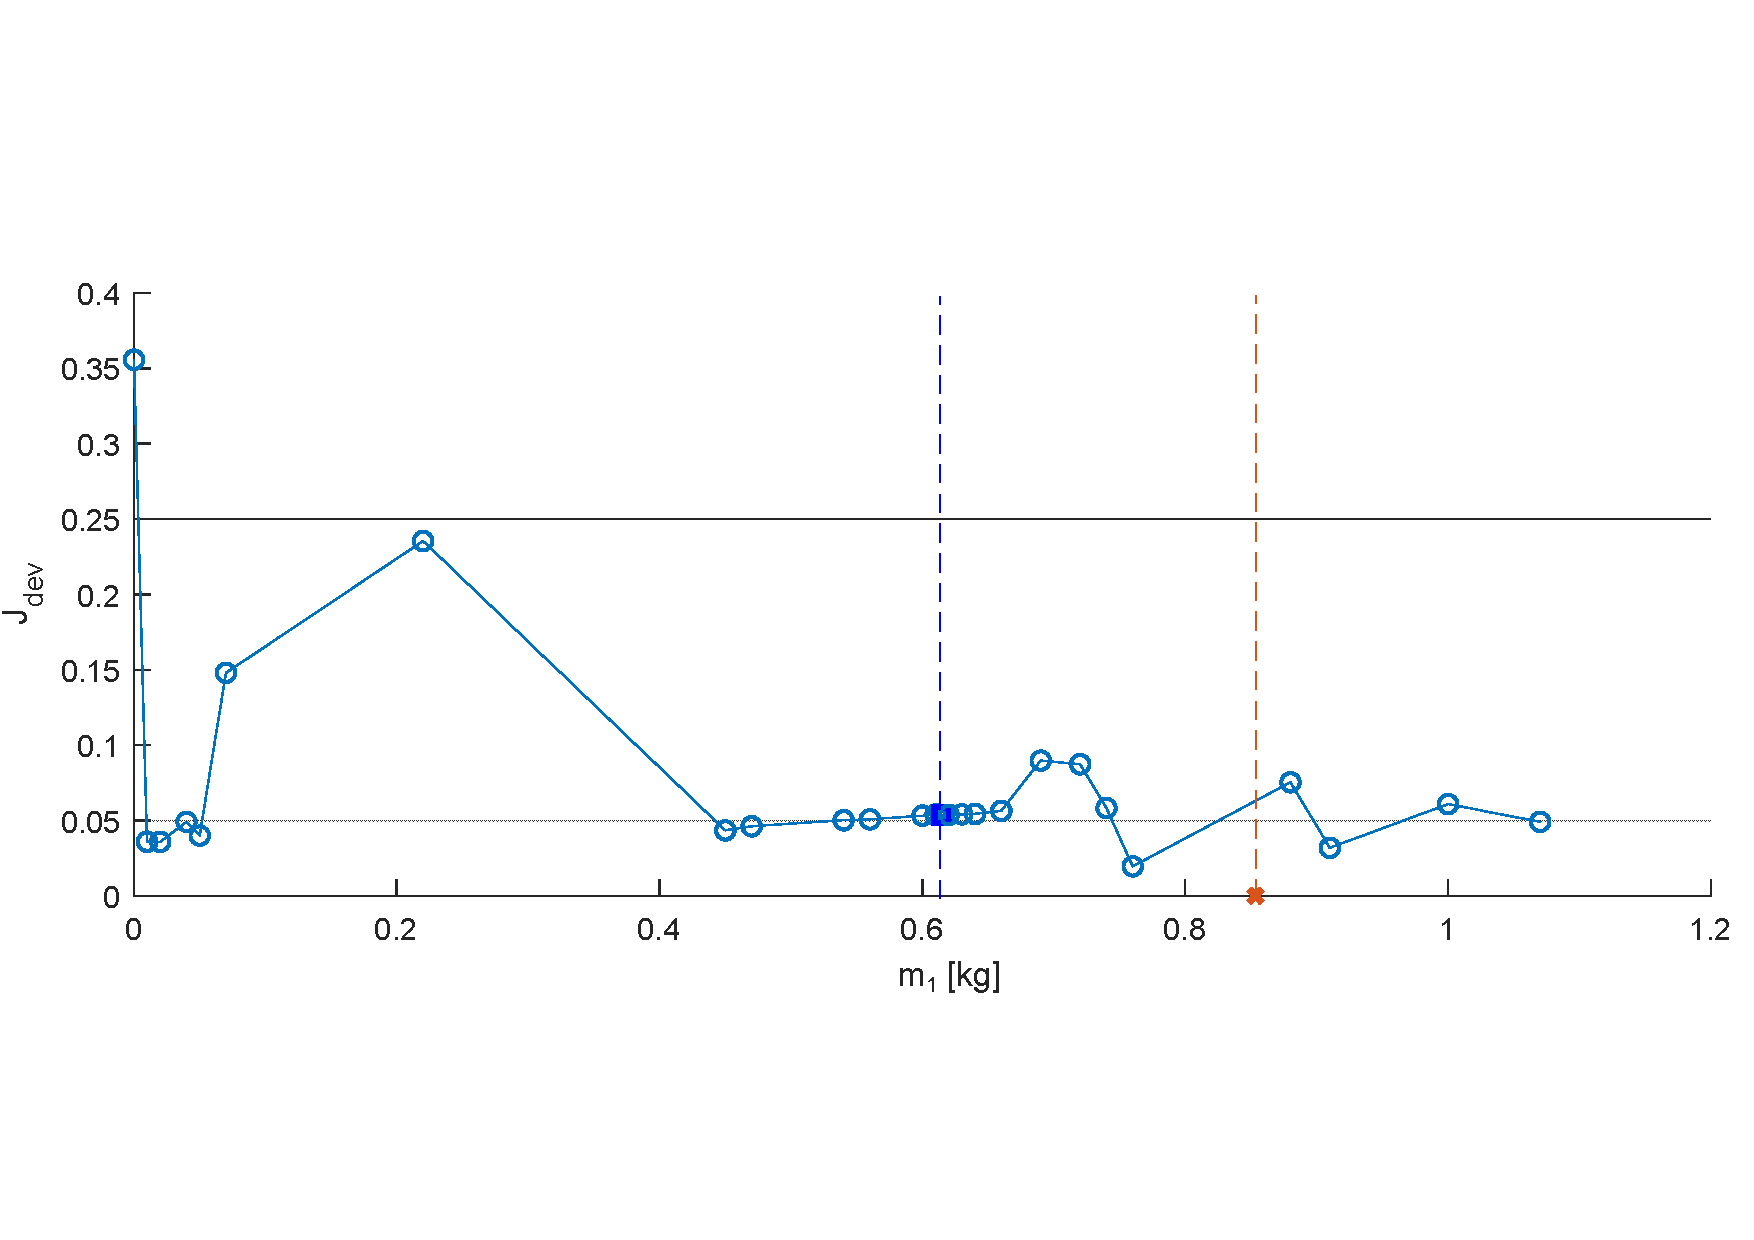
\includegraphics[width=0.8\textwidth]{Bilder/Trajektorien/m1.pdf}
	\caption{Variation $m_1$}
	\label{fig:trjvarm1} % etwas allgemein oder?
\end{figure}

Für $m_1$ lässt sich ein ähnliches Verhalten beobachten. Auch hier zeichnet sich der Bereich gültiger Trajektorien durch eine gut erkennbare Obergrenze ab. Diese liegt mit $m_{1\mrm{,max}}=\valunit{1,07}{kg}$ allerdings deutlich über der von $m_2$. Auffällig ist darüber hinaus eine Häufung gültiger Trajektorien mit hoher Güte im stark eingeschränkten Bereich $\valunit{0,6}{kg}\leq m_1 \leq\valunit{0,66}{kg}$ mit $\hg=88\%$, wo auch der Apprich-Wert einzuordnen ist. Bei einer Erweiterung des Bereichs auf $\valunit{0,45}{kg}\leq m_1 \leq\valunit{1,07}{kg}$ wird noch ein Anteil von $\hg=29\%$ erreicht. Eine ähnliche Häufung tritt im Bereich $\valunit{0}{kg}\leq m_1 \leq\valunit{0,07}{kg}$ mit $\hg=75\%$ auf, wobei die Bereichsgröße stark eingeschränkt ist. Allgemein liegen wie bei $m_2$ auch für $m_1$ die Trajektorien mit einer geringeren Güte von $J_\mrm{dev}<0,1$ im unteren Bereich. Besonders ungünstige Trajektorien mit $J_\mrm{dev}\gg1$ treten allerdings erneut nicht auf. Auch wird wieder für den Ribeiro-Parameter keine Lösung gefunden, wobei dieser nun in einem Bereich liegt, in dem prinzipiell Lösungen gefunden werden.

Allgemein wird als Wertebereich $\valunit{0}{kg}\leq m_1 \leq\valunit{1,07}{kg}$ formuliert, wobei $\Pkon\approx\hg=26 \%$ gilt. 

Anders als bei den Massen unterscheiden sich die Massenträgheitsmomente in ihrem Verhalten recht deutlich. Während für $J_1$ bezogen auf die Anzahl untersuchter Werte nur ein Anteil gültiger Trajektorien von $14 \%$ vorliegt, werden für $J_2$ mit einem Anteil von $61\%$ überwiegend gültige Trajektorien gefunden. Dies deutet auf einen geringen Einfluss von $J_2$ auf die Trajektorienberechnung hin. Die in \figref{fig:trjvarJ2} dargestellten Ergebnisse zeigen, dass beinahe über den gesamten Variationsraum von $J_2$ Trajektorien gefunden werden. Lediglich im untersten Bereich $\valunit{0}{kg m^2}\leq J_2 < \valunit{0,004}{kg m^2}$ können keine Trajektorien gefunden werden. In diesem Bereich ist der Ribeiro-Parameter angesiedelt, für den entsprechend keine Trajektorie gefunden wird. Der Apprich-Parameter befindet sich mit \valunit{0,00407}{kg m^2} unmittelbar im Grenzbereich. Durch eine Untergrenze der Wertebereichs mit $\valunit{0,004}{kg m^2}\leq J_2 \leq \valunit{0,02}{kg m^2}$ liegt der Anteil gültiger Trajektorien bei $77\%$. Wird die Untergrenze auf $J_{2\mrm{min}} = \valunit{0,0152}{kg m^2}$ erhöht, ergeben sich mit $\hg=100 \%$ ausschließlich gültige Trajektorien über den gesamten Bereich. Die Trajektoriengüte unterliegt im Bereich von $\hg=100 \%$ jedoch starken Schwankungen

\begin{figure}
	\centering
		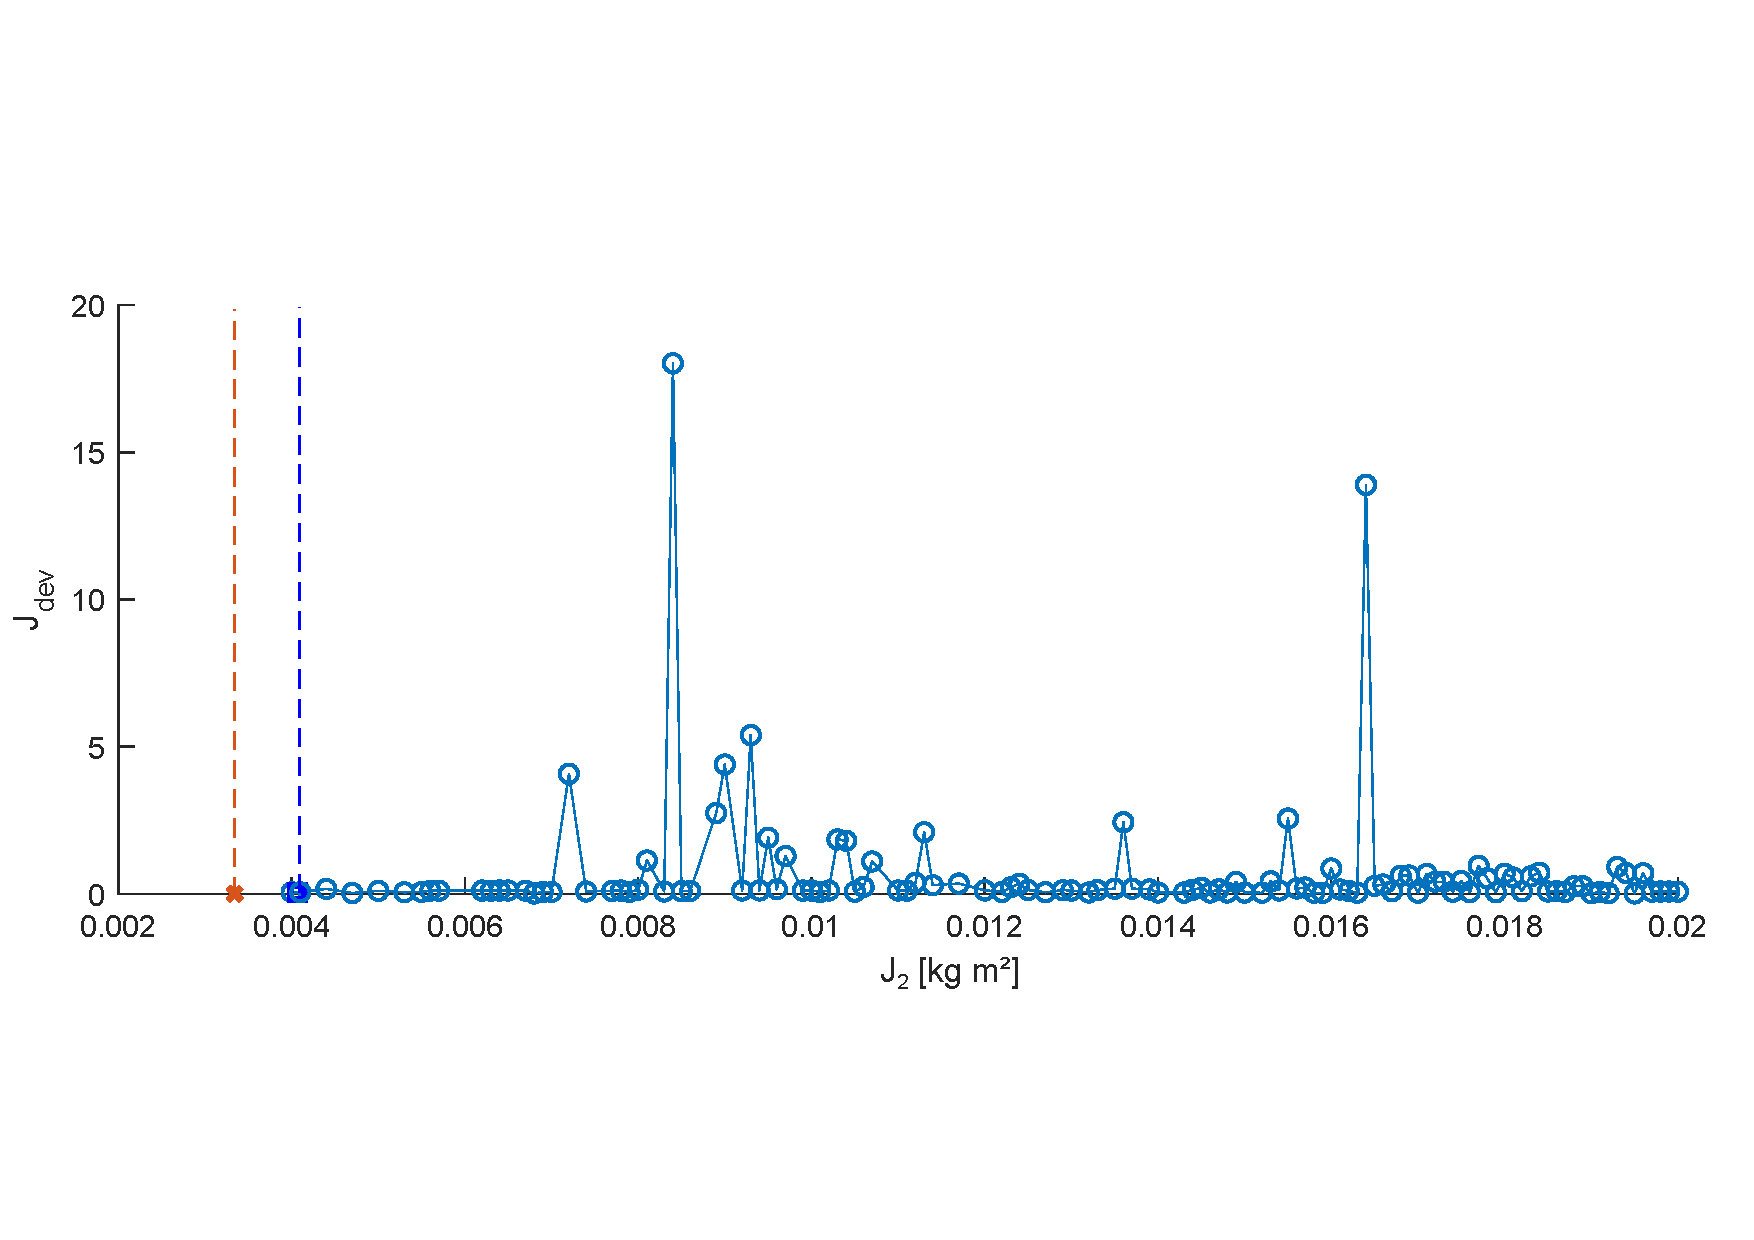
\includegraphics[width=0.8\textwidth]{Bilder/Trajektorien/J2.pdf}
	\caption{Variation $J_2$}
	\label{fig:trjvarJ2}
\end{figure}

Anders als bei den Stabmassen treten für $J_2$ erstmals besonders hohe Werte der Gütefunktion von $J_\mrm{dev}>>1$. Die für $J_2=\valunit{0,0084}{kg m^2}$ gefundene Trajektorie erreicht einen Wert von $J_\mrm{dev}=18,02$ und ist damit als unbrauchbar anzusehen. Im Bereich $\valunit{0,0072}{kg m^2}\leq J_2 \leq \valunit{0,0113}{kg m^2}$ tritt eine leichte Häufung von Trajektorien mit hohem $J_\mrm{dev}$ auf. Da es sich dennoch um lokale Minima und somit aus Sicht des Optimierers um gültige Trajektorien handelt, entsteht der hohe Wert weiterhin alleine aufgrund der hohen Ungenauigkeit der Approximation der Endlage. Für die weitere Verwendung berechneter Trajektorien ist daher dringend die Approximationsgüte zu überprüfen. Auch im beschriebenen Bereich von $\hg=100 \%$ treten vereinzelt gültige Trajektorien sehr geringer Güte auf.

Als Wertebereich gültiger Lösungen wird der Bereich $\valunit{0,004}{kg m^2}\leq J_2 \leq \valunit{0,02}{kg m^2}$ mit $\Pkon\approx\hg=77 \%$formuliert. Es wird zudem eine Erhöhung des aktuellen Ribeiro-Werts für $J_2$ empfohlen, sodass sich dieser zukünftig innerhalb des empfohlenen Wertebereichs befindet.

\begin{figure}
	\centering
		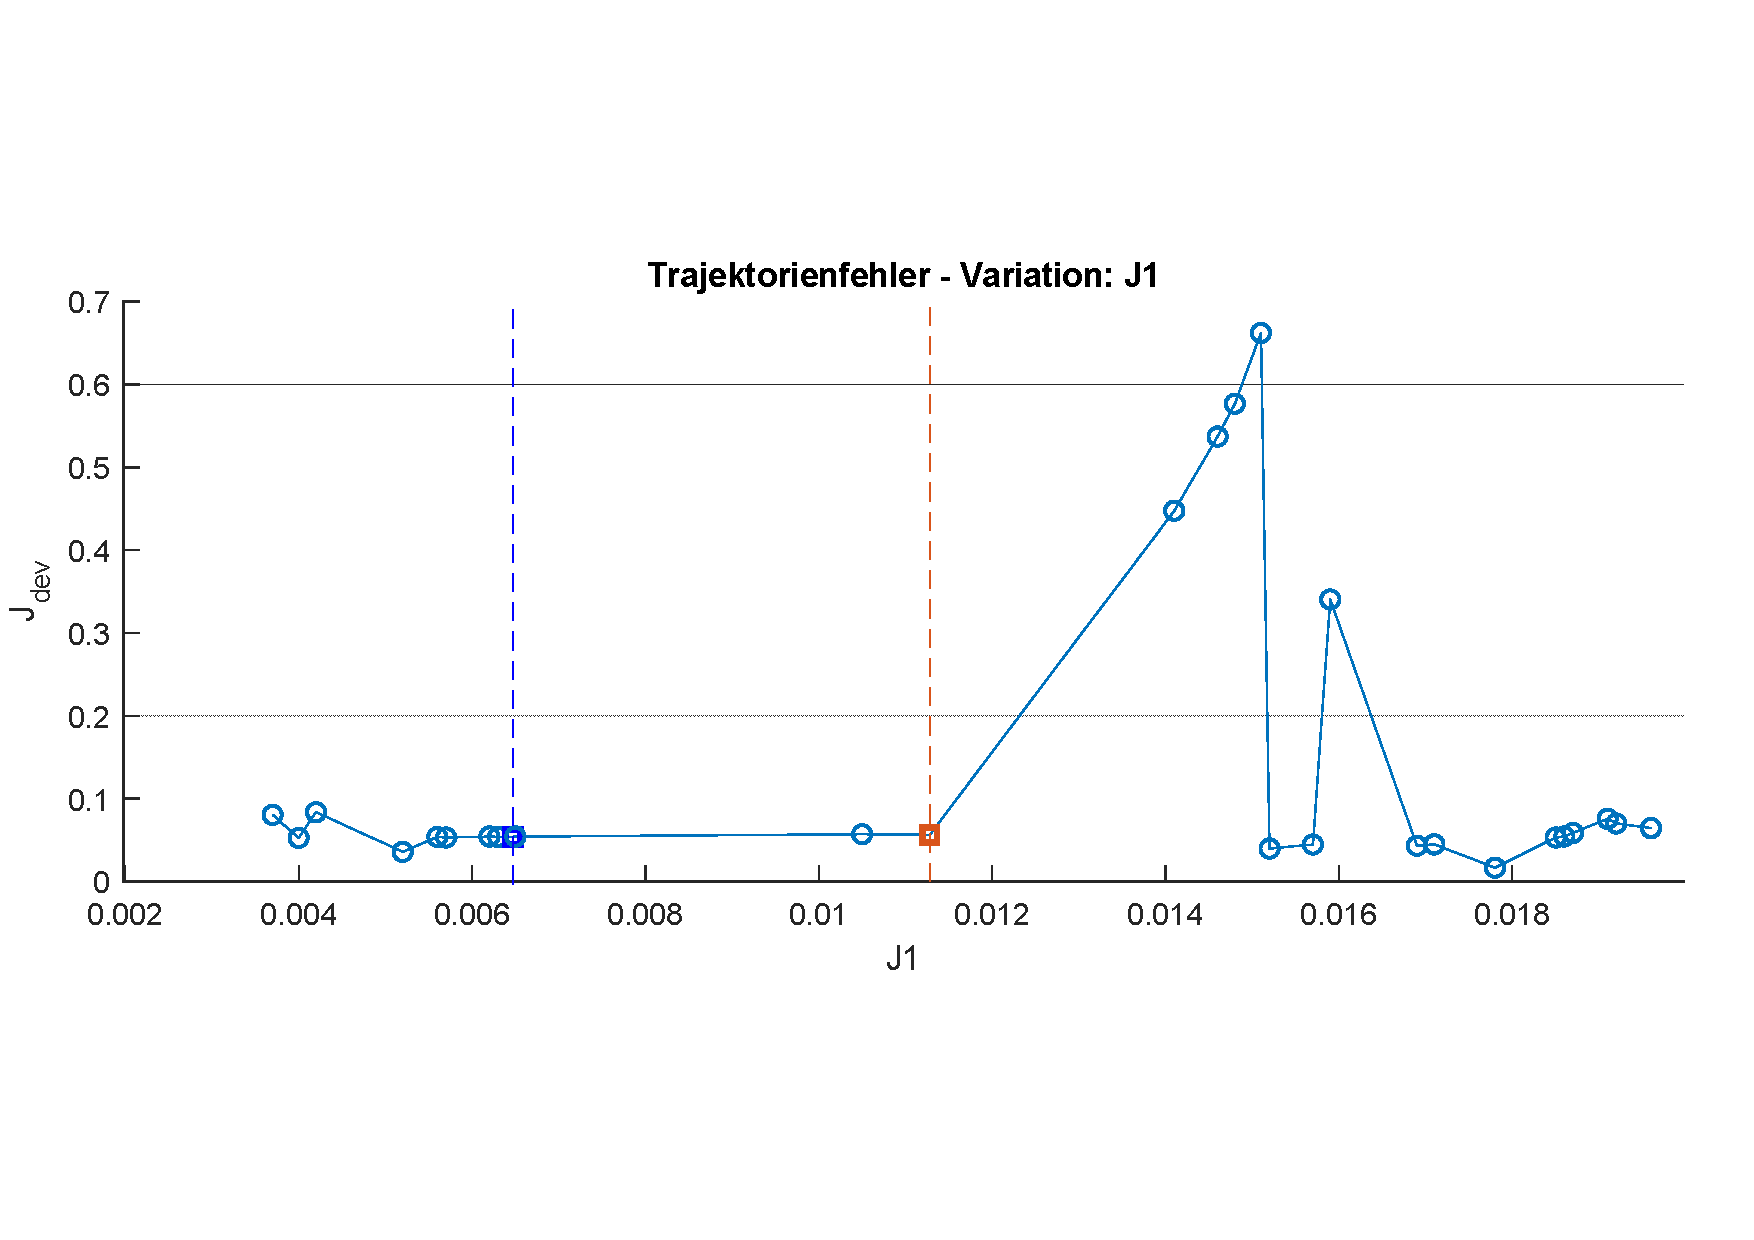
\includegraphics[width=0.8\textwidth]{Bilder/Trajektorien/J1.pdf}
	\caption{Variation $J_1$}
	\label{fig:trjvarJ1}
\end{figure}

Für $J_1$ werden mit insgesamt $\hg=14\%$ nur wenige gültige Trajektorien gefunden. Diese sind über den größten Teil des untersuchten Wertebereichs verteilt. Im Gegensatz zu den anderen Parametervariation wird hierbei auch eine Trajektorie für den Ribeiro-Wert gefunden. Dies lässt sich jedoch nicht mit einem Häufungsbereich weiterer gültiger Trajektorien begründen, wie \figref{fig:trjvarJ1} entnommen werden kann. Häufungen gültiger Trajektorien treten in den gegensätzlichen Bereichen $\valunit{0,0037}{kg m^2}\leq J_1 \leq \valunit{0,0065}{kg m^2}$ mit $\hg=33 \%$ und $\valunit{0,0141}{kg m^2}\leq J_1 \leq \valunit{0,0196}{kg m^2}$ mit $\hg=29 \%$ auf. Es können sich daher sowohl niedrige als hohe Werte für $J_1$ positiv auf die Konvergenz der Trajektorienberechnung auswirken. Der mittlere Bereich hingegen ist hingegen als ungünstig anzusehen, wobei dennoch gültige Lösungen gefunden werden können. Für sehr niedrige Werte existieren wie bei $J_2$ keine gültigen Trajektorien mehr, weshalb wieder eine Untergrenze $J_{2\mrm{min}} = \valunit{0,0037}{kg m^2}$ eingeführt wird.
Trajektorien mit $J_\mrm{dev}>1$ kommen anders als bei $J_2$ nicht vor. Ein erhöhtes Vorkommen von Trajektorien geringerer Güte mit $J_\mrm{dev}>0,1$ wird im Bereich $\valunit{0,0141}{kg m^2}\leq J_1 \leq \valunit{0,0159}{kg m^2}$ beobachtet. Da dieser Bereich wieder einen Grenzbereich einer Häufung gültiger Trajektorien markiert wie bei $m_1$ und $m_2$, könnte dies als Hinweis auf ein Verhaltensmuster der Güte verstanden werden. Die Variationen von $J_2$, $s_1$ und $s_2$ bestätigen diese Interpretation jedoch nicht.  

Mit der definierten Untergrenze wird ein Wertebereich für gültige Trajektorien von $\valunit{0,0037}{kg m^2}\leq J_2 \leq \valunit{0,0196}{kg m^2}$ mit $\Pkon\approx\hg=17 \%$ formuliert.

Aus der Variation der Schwerpunkte $s_1$ und $s_2$ wird kein auffälliges Verhalten identifiziert. Für beide Schwerpunkte können näherungsweise über die gesamte jeweilige Stablänge gültige Lösungen gefunden werden, sodass eine Eingrenzung des Wertebereichs nicht notwendig erscheint. Der Anteil gültiger Trajektorien ist für $s_1$ jedoch deutlich geringer als für $s_2$. Die Trajektorienberechnung reagiert damit prinzipiell empfindlicher auf eine Veränderung von $s_1$. Eine Häufung gültiger Trajektorien tritt wieder im Bereich des Apprich-Wertes auf. Obwohl der Ribeiro-Wert beider Schwerpunkte jeweils in einem solchen Häufungsbereich liegt, wird jeweils keine Trajektorie gefunden. Für die scheinbar ungünstigen Ribeiro-Schwerpunkte ist daher in diesem Fall keine explizite Ursache erkennbar.

Die formulierten Wertebereiche gültiger Trajektorien sind in \tabref{tab:Bereichsempfehlungen} noch einmal abschließend übersichtlich dargestellt. 
\begin{table}[h]
	\centering
	\caption{Wertebereiche gültiger Trajektorien}
		\begin{tabular}{lllll}
			\toprule
			Parameter  & Einfluss & min & max & $\Pkon$ \\
			\midrule
			{$m_1 \ [\unit{kg}]$}  &  hoch & $0$ & $1,07$  & $26 \%$ \\
			%\midrule			
			$m_2 \ [\unit{kg}]$  &  hoch & $0,09$ & $0,39$  & $38 \%$ \\	
			%\midrule
			$J_1 \ [\unit{kg m^2}]$  &  hoch & $0,0037$ & $0,0196$  & $17 \%$ \\
		  %\midrule
			$J_2 \ [\unit{kg m^2}]$ & gering & $0,004$ & $0,02$  & $77 \%$ \\
			%\midrule
			$s_1 \ [\unit{m}]$   &   mittel & $0$ & $0,29$  & $21 \%$ \\
			%\midrule
			$s_2 \ [\unit{m}]$   &   gering & $0$ & $0,338$  & $44 \%$ \\
			\bottomrule
		\end{tabular}
	\label{tab:Bereichsempfehlungen}
\end{table}

Es ist in Bezug auf die Ergebnisse zu berücksichtigen, dass die betrachteten Systemparameter jeweils für sich alleine variiert wurden. Eine Untersuchung bei Variation der Parameter in Abhängigkeit zu einander kann daher von den vorliegenden Ergebnissen abweichen. Ebenfalls sind die vielfältigen Konfigurationsmöglichkeiten der NMPC in Bezug auf die Ergebnisse zu problematisieren. Es ist entsprechend anzunehmen, dass formulierten Wertebereiche bei einer anderen Konfiguration der NMPC mit beispielsweise Variation von Schrittweite, Prädiktionshorizont, Integrator, Gewichtungsmatrizen der Gütefunktion oder anderem Optimierer variieren. Die formulierten Bereichsempfehlungen sind daher nur für die im Rahmen dieser Arbeit definierten Voraussetzungen gültig und in Bezug auf Allgemeingültigkeit in erster Linie als Orientierungshilfen, jedoch nicht als harte Grenzen zu verstehen. 

Die Gültigkeit der ermittelten Bereichsgrenzen muss außerdem für weitere Vergleichstrajektorien überprüft werden und gegebenenfalls trajektorienspezifische Grenzen formuliert werden. 

Die starke Begrenzung der Stabmassen lässt als Ursache eine verstärkte Abhängigkeit von der Stellgrößenbegrenzung vermuten.
Die Stellgrößenreserve bzw. die der NMPC als Nebenbedingung übergebene Kraftbegrenzung birgt somit ein weiteres Variationspotential, wodurch besonders eine Verschiebung der Bereichsobergrenzen zu erwarten ist. 

Die Coulomb-Reibung wurde im Rahmen der Untersuchung vernachlässigt. Erste Tests weisen auf einen erkennbar negativen Einfluss auf die Trajektorienbrechnung hin, was auf die hohe Nichtlinearität zurückgeführt wird. Wie in \secref{subsec:mitInd} werden hierzu verschiedene NMPC-Konfigurationen getestet, wobei lediglich für die Apprich-Parameter inklusive Coulomb-Reibung am Schlitten, exklusive Gelenkreibung, eine akzeptable Trajekorie gefunden wird, ebenfalls wieder für die bekannte NMPC-Konfiguration, die auch für die anderen Parametertests verwendet wurde. Es wird daher für zukünftige Arbeiten empfohlen, die für diese Arbeit gewählte Konfiguration weiterzuverwenden, wenn eine Variation der Reibwerte angestrebt wird.  




%\chapter{Einführung}\label{cha:Intro}
%
Beim Anfertigen einer Abschlussarbeit steht man als Studierender meist zum
ersten Mal vor dem Problem, einen längeren wissenschaftlichen Text mit Bildern,
Gleichungen und Referenzen schreiben zu müssen. Dafür bietet sich das
Textsatz-System \LaTeX\ an, zu dessen Vorteilen die weitgehende Trennung von
Inhalt und Layout gehören. Damit sich Studierende mehr mit dem \emph{Inhalt} der
Arbeit beschäftigen können, stellt das IAT ein \LaTeX-Dokument zur Verfügung, in
dem das \emph{Layout} der \verb|tudreport|-Klasse für das IAT angepasst wurde. Auch der vorliegende Text ist beispielhaft mit dieser Klasse geschrieben. \LaTeX-Grundlagen findet man \zB\ in \cite{Kopka}
oder \cite{Schmidt}. Allgemeines über
wissenschaftliche Arbeiten findet man in \cite{Friedrich}; als Einstieg in
die Typografie ist \cite{Willberg} sehr zu empfehlen.

Die Arbeit kann in Deutsch oder wahlweise auch in Englisch verfasst werden.

In der vorliegenden Anleitung werden in Kapitel \ref{cha:Hinweise} zuerst allgemeine Hinweise und Tipps zur Durchführung einer wissenschaftlichen Arbeit gegeben. Im Anschluß daran gibt Kapitel~\ref{cha:Hinweise_Latex} allgemeine Hinweise zum Erstellen der schriftlichen Arbeit. Es werden die \LaTeX-spezifischen Befehle vorgestellt, mit denen die Hinweise umgesetzt werden können. Die Hinweise in Kapitel~\ref{cha:Hinweise_Latex} sind auch für Studierende relevant, die sich gegen die Erstellung der Arbeit mit \LaTeX\ entscheiden. Da das Layout der Arbeit in diesem Fall zusätzlich selbst erstellt werden muss, dient die vorliegende Anleitung als Vorlage. In Kapitel \ref{cha:Verzeichnisstruktur} wird schließlich beschrieben, wie mit der \LaTeX-Vorlage gearbeitet werden sollte. 

Im Anhang findet sich eine Checkliste die vor Abgabe der Arbeit unbedingt abgearbeitet werden sollte, um zu prüfen, ob alle Vorgaben und Hinweise beachtet wurden.


%\chapter{Tipps für die Durchführung einer wissenschaftlichen Arbeit}
\label{cha:Hinweise}
%
%Eine wissenschaftliche Abschlussarbeit kann im Allgemeinen in die folgenden 4 Phasen gegliedert werden.
%
\section*{1. Phase: Einarbeitung und Literaturrecherche}
\label{sec:Einarbeitung}
\addcontentsline{toc}{section}{1. Phase: Einarbeitung und Literaturrecherche}
\begin{itemize}
	\item dient zur Verdeutlichung der gegebenen Problemstellung
	\item führt den Bearbeiter auf den \glqq{}State-of-the-Art\grqq{} hin $\rightarrow$ Literatur
	\item zeigt Möglichkeiten zur Problemlösung auf, die dann in Phase 2 genutzt werden können
	\item dient der Ideenfindung
	\item regelmäßige Treffen mit dem Betreuer
\end{itemize}


\section*{Generelles zu Treffen mit dem Betreuer}
\label{sec:TreffenBetreuer}
\addcontentsline{toc}{section}{Generelles zu Treffen mit dem Betreuer}
\begin{itemize}
	\item persönliche Treffen sollten gut vorbereitet werden (z.B. Fragenkatalog)
	\item Ergebnisse des Treffens und Anmerkungen des Betreuers festhalten (Notizen)
\end{itemize}


\subsection*{Literaturrecherche und -management}
\label{sec:Literaturrecherche}
\addcontentsline{toc}{subsection}{Literaturrecherche und -management}
Zur Sammlung und Verwaltung von Literatur dienen sog. Literaturdatenbanken. Diese Programme ermöglichen oft die direkte Verwendung als Literaturverzeichnis im späteren Text.

\emph{Empfehlung: JabRef (Freeware, auf Java-Basis, für alle Plattformen)}

Das Suchen und Lesen der aktuellsten Literatur ist wichtig für eine gute Übersicht über die
Problemstellung. Über die ULB ist es möglich viele Online-Quellen zu nutzen, um Texte auch als
pdf Dokumente erhalten zu können. Die für unseren Bereich wichtigsten Seiten sind:
\begin{itemize}
	\item \href{http://rzblx1.uni-regensburg.de/ezeit/}{Elektronische Zeitschriftenbibliothek} (DB aller Zeitschriften und Berechtigungen)
	\item \href{http://ieeexplore.ieee.org}{IEEEXplore} (Zugang zu allen Medien der IEEE)
	\item \href{http://www.sciencedirect.com}{Sciencedirect} (Zugang zu Zeitschriften aus dem ELSEVIER Verlag)
	\item \href{http://citeseerx.ist.psu.edu}{CiteSeer} (freie DB mit Zugang zu vielen Volltexten)
	\item \href{http://www.ifac-control.org/publications/ifac-papersonline.net}{IFAC-PapersOnline} (Archiv mit Artikeln aller IFAC Konferenzen)
	\item \href{http://link.springer.com/}{Springer E-Books} (Archiv des Springer Verlags mit vielen eBooks und Zeitschriften)
\end{itemize}
auch mal auf den Webseiten der Autoren schauen und natürlich \glqq{}googlen\grqq{}


\section*{2. Phase: Bearbeitung des Problems}
\label{sec:Bearbeitung}
\addcontentsline{toc}{section}{2. Phase: Bearbeitung des Problems}
\begin{itemize}
	\item dient zur Lösung der Problemstellung
	\item kreativste und anstrengendste Phase der Arbeit
	\item Verwendung professioneller Hilfsmittel (Programme wie Matlab oder Mathematica etc.)
	\item Treffen wenn Bedarf besteht, keine Regelmäßigkeit mehr
	\item sowohl die Implementierung als auch die Ausarbeitung/Präsentation sollten spätestens ab dieser Phase mittels eines Versionskontrollsystems wie \bspw \textsc{Git} oder \textsc{SVN} versioniert werden und regelmäßig zur Datensicherung auf einen externen Speicher übertragen werden, damit ältere (möglicherweise noch funktionsfähige) Stände wiederhergestellt werden können und keine Daten bei Zerstörung oder Verlust des Arbeitsrechners verloren gehen
\end{itemize}


\section*{3. Phase: Ergebnisse zusammen stellen}
\label{sec:Ergebnisse}
\addcontentsline{toc}{section}{3. Phase: Ergebnisse zusammen stellen}
\begin{itemize}
	\item dient der Reorganisation der Arbeit
	\item sämtliche Ergebnisse werden festgehalten
	\item Strukturierung und Gliederung der Ergebnisse, so dass die nächste Phase (Schreiben) gut durchgeführt werden kann
	\item wenige, längere Treffen zur Ergebnisbesprechung mit dem Betreuer
\end{itemize}


\subsection*{Ergebnissicherung}
\label{sec:Ergebnissicherung}
\addcontentsline{toc}{subsection}{Ergebnissicherung}
\begin{itemize}
	\item alles zusammentragen was erreicht wurde $\rightarrow$ guter Überblick notwendig (S.O.)
	\item auch Programmcode ist ein Ergebnis $\rightarrow$ verständlich kommentieren (Englisch)
	\item auf  Wiederverwendbarkeit von Grafiken achten (Linienstärke, Farbe, Beschriftung, \ldots)
	\item nur noch kleine Änderungen durchführen (z.B. Parametereinstellungen)
\end{itemize}
\emph{Ergebnisse sollten für sich sprechen und für jeden verständlich sein (ohne Erklärung)}


\section*{4. Phase: Dokumentation und Präsentation}
\label{sec:Dokumentation}
\addcontentsline{toc}{section}{4. Phase: Dokumentation und Präsentation}
\begin{itemize}
	\item Verfassen der Arbeit und erstellen der Präsentation
	\item letzte Verfeinerungen an den Ergebnissen (falls notwendig)
	\item schwierigste Phase der Arbeit
	\item regelmäßige Treffen zur Korrektur des Textes / der Präsentation
\end{itemize}

\newpage


\subsection*{Wissenschaftliches Schreiben}
\label{sec:Wissenschaftliches Schreiben}
\addcontentsline{toc}{subsection}{Wissenschaftliches Schreiben}
\begin{itemize}
	\item nicht am Layout der Arbeit aufhalten $\rightarrow$ Vorlage verwenden
	\item sehr aufwendiger Prozess von Schreiben - Verbessern - neu Schreiben - \ldots
	\item Aufwand darf nicht unterschätzt werden (Richtwert: 1-2 Seiten / Tag)
	\item einfach erst einmal aufschreiben -  korrigiert wird dann später
	\item Struktur einer wissenschaftlichen Arbeit ist vorgegeben
	\begin{itemize}
		\item \textbf{Titelseite} mit Art der Arbeit, Titel, Namen des Autors sowie Abgabedatum.
		\item \textbf{Aufgabenstellung} wird vom Betreuer der Arbeit zur Verfügung
		  gestellt.
		\item \textbf{Erklärung} zur Selbständigkeit. Der Text ist vorgegeben und wird bei Verwendung der Vorlage automatisch erzeugt.
		\item \textbf{Kurzfassung} der Arbeit.
		  Der Umfang soll so bemessen sein, dass die englische Version
		  (\textbf{Abstract}) auf die gleiche Seite passt.
		\item \textbf{Inhaltsverzeichnis} wird in \LaTeX{} durch \verb|\tableofcontents| automatisch
		  erzeugt.
		\item \textbf{Symbole und Abkürzungen}. Dieses Verzeichnis erstellt man am Besten von Hand. Die Einteilung in lateinische und griechische Symbole und Formelzeichen kann nach Bedarf geändert werden (zum Beispiel nach Kapiteln oder Konzepten) oder ganz weggelassen werden
		\item \textbf{Hauptteil der Arbeit}, in einzelne Kapitel und Abschnitte unterteilen.
		\item \textbf{Anhang}. Hier können Abschnitte stehen, die beim Lesen der Arbeit
		  stören würden, \zB\ Programmcode, technische Daten oder lange mathematische
		  Beweise.
		\item \textbf{Literaturverzeichnis} wird entweder von Hand erstellt oder automatisch generiert (in \LaTeX{} \zB mit.
		  \textsc{Bib}\TeX )
		\item \label{itm:Ordner} \textbf{Zusätzliches Material} wie \zB\ der
		  vollständige Programmcode eines Software-Projekts gehört nicht in die Arbeit,
	  sondern kann in einem separaten Ordner abgelegt werden.
	\end{itemize}
\end{itemize}
$P_\text{rägnanz}\; O_\text{rdnung}\; E_\text{infachheit}\; M_\text{otivation}$ (einfache, kurze, strukturierte und anregende Sätze)


\subsection*{Verteidigung und Präsentation}
\label{sec:Verteidigung}
\addcontentsline{toc}{subsection}{Verteidigung und Präsentation}
\begin{itemize}
	\item Inhalt der Arbeit auf ca. 10 wesentliche Punkte reduzieren
	\item je Punkt eine Folie maximal zwei
	\item je Folie 1-2 min Gesprächszeit
	\item Struktur der Präsentation:
	\begin{itemize}
		\item Motivation / Einleitung (Aufgabenstellung)
		\item Grundlagen
		\item Lösungsweg
		\item Ergebnisse
		\item Zusammenfassung (und Ausblick)
	\end{itemize}
	\item komplexe Sachverhalte durch Abbildungen verdeutlichen
	\item nur Stichpunkte schreiben, keine ganzen Sätze
	\item klare, einfach nachvollziehbare Notation (z.B. bei Variablen) verwenden
	\item mehrmaliges Üben des Vortrags (\zB vor dem Spiegel, vor der Familie, \ldots)
\end{itemize}
\emph{nichts weglassen was auf einer Folie steht, gerne zusätzliche Dinge erwähnen}


\section*{Organisatorisches}
\label{sec:Organisatorisches}
\addcontentsline{toc}{section}{Organisatorisches}
\begin{itemize}
	\item Bewertung
	\begin{itemize}
		\item Arbeitsstil: 40\% - Selbständigkeit, Verständnis, Kreativität, Fleiß, Zusammenarbeit mit Betreuer, Systematik
		\item Ergebnisse: 20\% - Qualität, Nutzbarkeit, Innovations-, Erfüllungsgrad
		\item Ausarbeitung: 30\% - Aufbau, äußere Form, Sprache, Grundlagen, Vollständigkeit
		\item Vortrag: 10\% - Inhalt, Stil, Folien, Vorführung, Diskussion
	\end{itemize}
	\item jeder Studierende sollte an mindestens einem Regelungstechnischen Seminar teilnehmen
	\item Abgabetermin ist ein fixer Termin $\rightarrow$ Prüfungsleistung (Durchfallen möglich)
	\item jeder Studierende erhält auf Wunsch einen eigenen Account für unsere Rechner (Passwort legt Admin fest)
	\item zur Erstellung der Ausarbeitung und der Präsentation wird die Verwendung des Textsatzprogramms \LaTeX empfohlen, das Template für die Ausarbeitung erhaltet Ihr vom Betreuer
\end{itemize}


\section*{Allgemeines zu Hilfsmitteln bei der Erstellung und Bearbeitung}
\label{sec:Allgemeines}
\addcontentsline{toc}{section}{Allgemeines zu Hilfsmitteln bei der Erstellung und Bearbeitung}
\begin{itemize}
	\item es gibt viele Bücher die bei der Erstellung von wissenschaftlichen Arbeiten helfen
	\item viele verwendete Programme bieten ausführliche Hilfen an (z.B. \Matlab, Mathematica)
	\item bei Problemen immer zuerst in der Hilfe schauen, dann "googlen", dann Betreuer fragen
\end{itemize}


\subsection*{Empfohlene Programme}
\label{sec:Empfohlene Programme}
\addcontentsline{toc}{subsection}{Empfohlene Programme}
\begin{itemize}
	\item Literaturdatenbank $\rightarrow$ JabRef (http://jabref.sourceforge.net/)
	\item Ausarbeitung und Präsentation $\rightarrow$ \LaTeX / PowerPoint
	\item Simulation und Regelungstechnik $\rightarrow$ \MatSim
	\item symbolische und numerische Berechnungen $\rightarrow$ Mathematica
	\item Plots $\rightarrow$ \texttt{pgfplots}
	\item Blockschaltbilder $\rightarrow$ \texttt{TikZ}
	\item Versionskontrolle $\rightarrow$ \textsc{Git}
\end{itemize}

%\chapter{Allgemeine Hinweise und Informationen zum Erstellen einer schriftlichen Arbeit mit \LaTeX}
\label{cha:Hinweise_Latex}

%Dieses Kapitel gibt allgemeine Hinweise zur Erstellung einer wissenschaftlichen Arbeit mit dem Textsatzprogramm \LaTeX. Es ist inhaltlich identisch mit dem vorherigen Kapitel und enthält zusätzlich die \LaTeX-spezifischen Befehle, die bei der Umsetzung der Hinweise hilfreich sein könnten.

%Wird die Arbeit \emph{nicht} mit \LaTeX\ erstellt, sollte das vorherige Kapitel gelesen werden.

%Besonderes Augenmerk sollte auf Abschnitt~\ref{sec:Latex-Zitieren}, \textbf{Zitate und korrekte Zitierweisen} gelegt werden.

Dieses Kapitel gibt allgemeine Hinweise zur Erstellung einer wissenschaftlichen Arbeit mit dem Textsatzprogramm \LaTeX. Das Kapitel sollte auch von Studierenden gelesen werden, die sich gegen eine Erstellung der Arbeit mit \LaTeX\ entschieden haben. Da das Layout der Arbeit in diesem Fall gemäß den TUD Designvorgaben zusätzlich selbst erstellt werden muss, dient die vorliegende Anleitung auch als Vorlage.

%Wird die Arbeit \emph{nicht} mit \LaTeX\ erstellt, sollte das vorherige Kapitel gelesen werden.

%Besonderes Augenmerk sollte auf Abschnitt~\ref{sec:Latex-Zitieren}, \textbf{Zitate und korrekte Zitierweisen} gelegt werden.

\section{\LaTeX-Distribution}
\label{sec:Distribution}
Welche Distribution verwendet wird, hängt vom persönlichen Geschmack des Anwenders ab und es besteht grundsätzlich die Wahl zwischen \Miktex{}, das vor allem unter Windows weit verbreitet ist und \texlive{}, das eher unter Linux und Mac Anwendung findet.
Im Folgenden wird nur das Vorgehen für \Miktex{} unter Windows beschrieben, für \texlive{} sind die Abläufe ähnlich.

Zuerst ist die Distribution herunterzuladen und zu installieren, wobei im Allgemeinen die Standardeinstellungen ausreichend sind.


\section{Editor}
Für \LaTeX{} gibt es eine Vielzahl von freien und kommerziellen Texteditoren. Das \Texstudio ist ein freier open-source Editor, der sich bei uns am Institut bewährt hat.

\subsection{Einrichten von \Texstudio}
Es gibt prinzipiell zwei verschiedene Wege, um aus der \LaTeX-Quelldatei ein pdf zu erzeugen.
\begin{itemize}
	\item \LaTeX => PDF pdf\LaTeX{} wandelt die Quelldatei direkt in ein pdf.
	Dabei können als Bilder im Format .jpg, .png und .pdf eingebunden werden.
\end{itemize}
In \Texstudio{} kann die Werkzeugkette im Reiter \zitat{Erzeugen} in den Einstellungen angepasst werden.
Um das direkte Kompilieren mit pdf\LaTeX{} zu verwenden ist bei Kompiler \texttt{txs:///pdflatex} einzutragen, während für den Weg über Postscript \texttt{txs:///latex} einzutragen ist.
\Texstudio{} verwendet eine Hauptdatei für die Kompilierung, die entweder automatisch ermittelt wird, oder vom Benutzer festgelegt wird.

\subsubsection{Autovervollständigung}
Damit die Makros in den Paketen, die mit der Vorlage mitgeliefert werden, von \Texstudio{} beim Eintippen automatisch ergänzt werden, müssen die in den Ordnern der jeweiligen Pakete befindlichen cwl-Dateien in den Ordner \verb|%APPDATA%/TeXstudio/completion/user| kopiert werden und \Texstudio{} neu gestartet werden.
Durch Anlegen einer eigenen cwl-Datei können dort auch eigene Autovervollstädigungen definiert werden, wie in der Dokumentation unter \url{http://texstudio.sourceforge.net/manual/current/usermanual_en.html#CWLDESCRIPTION} nachzulesen ist.
Sollen die Vervollständigungen dauerhaft aktiviert werden und nicht nur, wenn \Texstudio{} das Laden der entsprechenden Pakete erkannt hat, ist unter \Texstudio{} konfigurieren->Vervollständigung ein Haken bei der gewünschten cwl-Datei zu setzen.

\subsubsection{Makros}
Da das Öffnen von Dateien, die mit dem Makro \texttt{\textbackslash{}inputtikz} geladen werden, in \Texstudio{} nicht mehr über die eingebaute Funktionalität möglich ist, kann das das Javascriptmakro \texttt{open\_includetikz.js} über \zitat{Makros->Makros bearbeiten} durch Kopieren in das sich öffnende Fenster hinzugefügt werden und ein beliebiges Tastenkürzel mit diesem assoziiert werden, damit sich die eingebundenen Bilddateien bei Eingabe des Tastenkürzels öffnen, wenn der Curser in einer Zeile mit dem Makronamen steht.



\section{Rechtschreibung}

Studentische Abschlussarbeiten am IAT sind nach den aktuell geltenden Regeln der deutschen Rechtschreibung zu verfassen, \cite{Duden}.

Die neue deutsche Rechtschreibung wird in \LaTeX\ mit dem Paket \verb|babel| über die Option \verb|ngerman| aktiviert.

Im Internet findet man unter \url{http://www.duden.de/} einen Crashkurs zur neuen deutschen Rechtschreibung.

Eine Überprüfung der Rechtschreibung über die in die Editoren eingebaute Rechtschreibprüfung hinaus, lässt sich in \Texstudio{} mit dem Languagetool erreichen.
Dieses kann unter \Texstudio{} im Reiter \zitat{Sprache prüfen} konfiguriert werden.
Dort ist unter \zitat{LT-Pfad} der Pfad zur jar-Datei \texttt{languagetool.jar} anzugeben und unter \zitat{LT-Argumente} \zitat{\texttt{org.languagetool.server.HTTPServer -p 8081}} und bei \zitat{Server-Adresse} \zitat{\texttt{http://local\-host:8081}} einzugeben.
Zum Einschalten der Überprüfung kann dann vor dem Starten von \Texstudio{} das Languagetool von Hand gestartet werden, oder über \zitat{Starte das Languagetool falls es nicht läuft} automatisch gestartet werden.


\section{Zitate und korrekte Zitierweise}
\label{sec:Latex-Zitieren}
Zitate sind wörtliche oder sinngemäße Wiedergaben von Gedanken, Ideen oder Meinungen anderer Autoren.
Werden Ideen oder Inhalte aus Quellen wörtlich oder sinngemäß in die eigene Arbeit übernommen, besteht die \textbf{Pflicht}, diese zu kennzeichnen.
Wird dies unterlassen, liegt ein \textbf{Täuschungsversuch} (Plagiat) vor und die Arbeit kann als \textbf{nicht bestanden} bewertet werden.

Laut § 38 Abs. 2 der \emph{Allgemeinen Prüfungsbestimmungen} liegt \glqq\ [...] ein Täuschungsversuch [...] vor, wenn eine falsche Erklärung nach §§ 22 Abs. 7, 23 Abs. 7 abgegeben worden ist oder ein anderes Werk, eine Bearbeitung eines anderen Werkes, eine Umgestaltung eines anderen Werkes ganz oder teilweise in der Prüfungsarbeit wiedergeben werden, ohne dieses zu zitieren (Plagiat).\grqq~\cite{APB}

\subsection*{Zitierfähigkeit}
Zitierfähig sind nur veröffentlichte Werke aus allgemein zugänglichen Quellen (Bücher, Artikel, \etc).
Quellen, bei denen die Verfügbarkeit nicht garantiert werden kann (Internetquellen) oder der Urheber nicht klar nachvollziehbar ist (Wikipedia, o\,Ä.), sind problematisch und sollten möglichst vermieden werden.
Wird doch solch eine Quelle zitiert, ist die aktuelle Version zum Zeitpunkt des Zitates beizulegen.

\subsection*{Wörtliche Zitate}
Wörtliche Zitate in ingenieurwissenschaftlichen Arbeiten sind unüblich.
Sollte doch ein wörtliches Zitat in die Arbeit übernommen werden, muss dieses buchstaben- und zeichengetreu, inklusive eventueller Rechtschreibfehler übernommen werden.
Das wörtliche Zitat wird in Anführungszeichen eingefasst.

\subsection*{Sinngemäße Zitate}
Weit häufiger werden in wissenschaftlichen Arbeiten Ideen oder Meinungen anderer Autoren sinngemäß übernommen.
Diese müssen durch einen Verweis auf die Quelle gekennzeichnet werden.
Durch die Position des Verweises muss der Umfang der sinngemäßen Übernahme klar hervorgehen.

\subsection*{Quellenangaben im Literaturverzeichnis}
Für die Darstellung der Verweise, als auch für die Darstellung der Quellen im Literaturverzeichnis gibt es verschiedene Zitierweisen.
Üblich sind die Harvard-Variante mit Autor und Veröffentlichungsjahr in runden Klammern, wie zum Beispiel (Isermann, 2001) oder eine fortlaufende Nummerierung in eckigen Klammern, wie in dieser Vorlage.
Das \texttt{biblatex} Paket ermöglicht verschiedene (im Deutschen übliche) Zitierweisen.
Die Sortierung des Literaturverzeichnisses kann alphabetisch (voreingestellt, oder \bspw durch die Paketoption \texttt{sorting=nyt}) oder nach dem Erscheinen der Verweise erfolgen (durch die Paketoption \texttt{sorting=none}).
Das Paket \texttt{iatsada} definiert einen Zitierstil basierend auf dem \texttt{numeric} Stil von \texttt{biblatex}, kann aber bei Bedarf angepasst werden, falls \bspw ein alphabetischer Stil (\texttt{alphabetic}) vorgezogen wird.

Ein Verweis wird mit \texttt{\textbackslash{}cite\{$\left\langle\text{label}\right\rangle$\}} eingefügt und mit einem festen Leerzeichen \verb|~| mit dem vorherigen Wort getrennt.
Schließt der Verweis einen Satz ab, folgt der Punkt \emph{hinter} dem Verweis.
Neben dem \texttt{\textbackslash{}cite} Befehl stehen im Paket \texttt{iatsada} weitere Makros zur Zitierung von Seitenzahlen wie \texttt{\textbackslash{}citep\{$\left\langle\text{label}\right\rangle$\}\{$\left\langle\text{page}\right\rangle$\}} oder \texttt{\textbackslash{}citerange\{$\left\langle\text{label}\right\rangle$\}\{$\left\langle\text{pageu}\right\rangle$\}\{$\left\langle\text{pageo}\right\rangle$\}} zur Verfügung, die vorgezogen werden sollte, da der Leser so, vor allem bei umfangreicheren Werken, schneller den zitierten Sachverhalt nachlesen kann.

Die Literaturliste wird \LaTeX{} über eine Datei im \textsc{Bib}\TeX{}-Format mit der Endung \texttt{bib} bekannt gemacht.
Für die Erstellung des Literaturverzeichnisses (Datei mit der Endung \texttt{bbl}) aus der Literaturliste bietet sich die Erweiterung \textsc{Biber} an, die mit der Paketoption \texttt{backend=biber}\footnote{\label{ftn:Fussnote1}Alternativ kann auch \texttt{backend=bibtex} verwendet werden, wobei dann die Werkzeugkette des verwendeten Editors entsprechend eingestellt werden muss.} in \texttt{biblatex} geladen werden kann und im Editor in die entsprechende Werkzeugkette integriert werden muss, damit \textsc{Biber} ausgeführt wird.
Alternativ kann das Literaturverzeichnis auch per Hand erstellt werden.
Viele Literaturverwaltungsprogramme, wie zum Beispiel \textsc{JabRef}, ermöglichen den direkten Export der Datenbank in das \textsc{Bib}\TeX{}-Format.


\section{Gliederung des Dokuments}
\label{sec:Latex-Gliederung}
Im Inhaltsverzeichnis wird die Gliederung der Arbeit dargestellt. Die Überschriften und Seitenangaben der Kapitel, Unterkapitel und Abschnitte müssen mit den Elementen im Inhaltsverzeichnis übereinstimmen. Überschriften sind kurz und prägnant zu formulieren und dürfen keine vollständigen Sätze sein. Gibt es Unterpunkte in der Gliederung, so müssen immer mindestens zwei davon existieren und inhaltlich auf der gleichen Ebene sein. Die einzelnen Punkte des Inhaltsverzeichnis müssen nummeriert werden. Die Übersichtlichkeit des Inhaltsverzeichnisses kann durch Einrücken der Unterpunkte erhöht werden.

Das Inhaltsverzeichnis wird in \LaTeX\ automatisch erstellt.
Innerhalb der einzelnen Kapitel \verb|\chapter{...}| werden weitere Unterteilungen mit den Befehlen \verb|\section{...}|, \verb|\subsection{...}| \usw vorgenommen.
Werden diese mit einem \verb|*| versehen, dann erhält der jeweilige Abschnitt keine Nummer und erscheint nicht im Inhaltsverzeichnis.
Dies kann in manchen Fällen nützlich sein.

Um eine korrekte Darstellung des Inhaltsverzeichnisses zu erhalten, muss \ggf mehrmals hintereinander kompiliert werden, da sich aufgrund von
Gleitobjekten Seitenzahlen ändern können.
Dreimaliges Kompilieren reicht in der Regel.

Bei Bildern und Tabellen, die in eine \verb|figure|- bzw.\ \verb|table|-Umgebung eingeschlossen sind, handelt es sich um sog.\ \emph{Gleitobjekte}, \dah sie erscheinen nicht an der Stelle, an der sie eingebunden werden, sondern oben oder unten auf einer Seite, siehe \zB \tabvref{tab:Sonderzeichen}.
Optional können in \verb|[]| noch Positionierungswünsche angegeben werden.
Mit dem Befehl \verb|\caption{...}| erhalten Bilder eine \emph{Unterschrift} und Tabellen eine \emph{Überschrift}.

Kapitel, Abschnitte, Bilder, Tabellen und Gleichungen können mittels \verb|\label{...}| benannt werden.
Dadurch ist es möglich, sie später mit \verb|\ref{...}| oder \verb|\pageref{...}| zu referenzieren.
Es empfiehlt sich, den Namen (Labels) eine Markierung voranzustellen, aus der hervorgeht, um welches Objekt es sich handelt.
Üblich sind \verb|cha:| für \glqq Chapter\grqq, \verb|sec:| für \glqq Section\grqq, \verb|fig:| für \glqq Figure\grqq, \verb|tab:| für \glqq Table\grqq\ und \verb|eq:| für \glqq Equation\grqq.
Ein Bild benennt man also \zB\ mit \verb|\label{fig:Ausgangssignal}|.
Für die verschiedenen Arten von Objekten bietet das Paket \texttt{iatsada} die in \tabref{tab:Referenzen} angegebenen speziellen Referenzierungsmakros.
\begin{table}
	\centering
	\caption{Labels und zugehörige Referenzen}
	\label{tab:Referenzen}  
	\begin{tabular}{llll}
		Typ			&	Prefix				&	Referenz			&	resultierender Text\\
    \midrule
		Chapter		&	\texttt{cha}		&	\verb|\charef|		&	\charef{cha:Hinweise_Latex}\\
		Section		&	\texttt{sec}		&	\verb|\secref|		&	\secref{sec:Latex-Gliederung}\\
		Anhang		&	\texttt{cha/sec}	&	\verb|\appref|	&	\appref{cha:Checkliste}\\
		Table		&	\texttt{tab}		&	\verb|\tabref|		&	\tabref{tab:Referenzen}\\
		Figure		&	\texttt{fig}		&	\verb|\figref|		&	\figref{fig:Standardregelkreis}\\
		Equation	&	\texttt{eq/equ}		&	\verb|\equref|		&	\equref{eq:Allgemein-Approx}\\
		Listing		&	\texttt{lst}		&	\verb|\lstref|		&	\lstref{lst:Listing1}\\
		Algorithm	&	\texttt{alg}		&	\verb|\algoref|		&	\algoref{lst:Listing1}\\
		Footnote	&	\texttt{ftn}		&	\verb|\ftnref|		&	\ftnref{ftn:Fussnote1}\\
    \midrule
		Table		&	\texttt{tab}		&	\verb|\tabvref|		&	\tabvref{tab:Systemparameter}\\
		Figure		&	\texttt{fig}		&	\verb|\figvref|		&	\figvref{fig:Standardregelkreis}\\
    \bottomrule
	\end{tabular}
\end{table}

\section{Bilder}
\label{sec:Latex-Bilder}

Wenn möglich, sollten Bilder als Vektorgrafik eingebunden werden, damit sichergestellt werden, dass alle Details beim Ausdrucken erhalten bleiben.
Es ist dabei auf eine ausreichende Strichstärke zu achten.
Ebenfalls sollten die im Bild verwendete Schrift die gleiche sein, wie im übrigen Dokument.

Werden doch Pixelgrafiken verwendet, so ist die richtige Wahl der Auflösung von besonderer Bedeutung.
Einerseits sollten die Bilder auf dem ausgedruckten Dokument gut aussehen, andererseits aber auch eine zügige Bildschirmdarstellung und kleine Dateigröße ermöglichen.


Für die Erstellung von Plots eignet sich das \LaTeX-Paket \texttt{pgfplots} sehr gut.
In \appref{cha:Anhang-Grafiken} sind weitere geeignete Programme zur Erstellung von Bildern und Plots mit ihren Eigenschaften aufgelistet.

Eine Grafik lässt sich am einfachsten mit dem Befehl \verb|\includegraphics{}| aus dem \verb|graphicx|-Paket einbinden.
Eine vollständige Beschreibung des Befehls und weiterer nützlicher Grafikbefehle findet man in der Dokumentation des \verb|graphicx|-Pakets.
Diese liegt -- wie die Beschreibung aller anderen \LaTeX-Pakete -- im \verb|doc|-Verzeichnis des \TeX-Systems und kann mit \texttt{texdoc $\left\langle\text{paketname}\right\rangle$} aufgerufen werden.
In welchem Format \verb|graphicx| die Grafiken benötigt, hängt davon ab, ob man \TeX\ in Verbindung mit \textsc{Dvips} verwendet oder stattdessen pdf\TeX, siehe \appref{cha:TexSystem}.

\textbf{pdf\TeX} (empfohlen) verarbeitet dagegen Grafiken im \emph{Portable-Document-Format} (\verb|*.pdf|) sowie die Pixelformate \texttt{jpeg} und \texttt{png}.
Den direkten Export von PDF-Grafiken bieten derzeit zwar nur wenige Programme an, sie lassen sich aber einfach aus dem EPS-Format mit Hilfe des Acrobat Distiller oder Ghostscript erzeugen.
Zum Einbinden von EPS-Dateien muss das Paket \texttt{epsfig} geladen sein.

Für \textbf{\TeX/Dvips} müssen alle Grafiken im \emph{Encapsulated-PostScript}-Format (\verb|*.eps|) vorliegen.
EPS-Dateien lassen sich aus praktisch jeder Software erzeugen und können sowohl Vektor- als auch Pixelgrafiken enthalten -- zusätzlich sind auch Preview-Grafiken möglich, was aber in der \TeX-Welt im Allgemeinen nicht erforderlich ist.

Bilder müssen zentriert sein (\verb|\centering|) und eine Bild\emph{unterschrift} (\verb|\caption{...}|) besitzen.
Um auf eine Abbildung zu referenzieren, kann auch sie mit einem \verb|\label{fig:...}| versehen werden.
Nur in besonderen Ausnahmefällen sollten Bilder mit Text umflossen werden.
Wurden Abbildungen einer Quelle entnommen, muss dies entsprechend mit einem Verweis auf die Quelle im Literaturverzeichnis gekennzeichnet werden.
Wenn dazu das Makro \verb|\cite| verwendet wird, so ist zusätzlich das optionale Argument von \verb|\caption| ohne den Literaturverweis zu verwenden, damit die Verlinkungen im Abbildungsverzeichnis nicht zerstört werden.
Werden Abbildungen eine Quelle nachempfunden, angepasst oder abgeändert, ist dies mit dem Zusatz \glqq in Anlehnung an...\grqq\ oder ähnlich anzugeben.

\begin{figure}[htp]
	\centering
	\begin{tikzpicture}[node distance=5mm and 10mm]
	\node[terminal]	(w)	{};
	\node[sum]			(s) [right=of w]	{};
	\node[block]		(Regler) 		[right=of s] 			 	{Regler};
	\node[block]		(Aktor)	 		[right=of Regler]  	{Aktor};
	\node[block]		(Strecke)		[right=of Aktor]	 	{Strecke};
	\node[branch]		(punkt)			[right=of Strecke] 	{};
	\node[terminal]	(y)					[right=of punkt]		{};
	\node[block]		(Messglied) [below=of Aktor]		{Messglied};
	
	
	\draw[to] (w) -- (s) node[near start,above] {$w$};
	\draw[to] (s) -- (Regler) node[midway,above] {$e$}; 
	\draw[to] (Regler) -- (Aktor);
	\draw[to] (Aktor) -- (Strecke);
	\draw[to] (Strecke) -- (y) node[pos=0.8,above] {$y$};
	\draw[to] (punkt) |- (Messglied);
	\draw[to] (Messglied) -| (s) node[pos=0.95, right] {-};
\end{tikzpicture}
	\caption{Standard-Regelkreis; Bild erstellt mit \texttt{TikZ}}
	\label{fig:Standardregelkreis}
\end{figure}

Generell ist die Arbeit (und insbesondere die Grafiken) so zu gestalten, dass sie auch schwarzweiß gedruckt werden kann.
Farbige Fotos und Screenshots verursachen dabei \iA keine zusätzlichen Probleme.
Werden jedoch \zB farbige Kurven in einem Diagramm dargestellt, hat dies folgende Konsequenzen:
\begin{itemize}
	\item Keine zu hellen Farben für die Linien verwenden, da diese sonst beim Drucken nicht zu erkennen sind.
	RGB-Grün $(0,1,0)$ ist tabu!
	\item Bei mehreren Kurvenverläufen darf deren Farbe nicht das einzige Unterscheidungsmerkmal sein: Entweder sind unterschiedliche Linienformen zu verwenden oder die Kurven im Diagramm beschriften.
\end{itemize}

Bei der Erstellung von Plots ist unbedingt die \href{http://de.wikipedia.org/wiki/DIN_461}{\texttt{DIN 461 Grafische Darstellung in Koordinatensystemen}} zu beachten.
Hilfreich in diesem Zusammenhang und überhaupt für die korrekte Schreibweise von Zahlen und Einheiten im Fließtext und in Formeln sind die Hinweise der TU-Chemnitz: \url{www.tu-chemnitz.de/physik/FPRAK/Grundsatz/Literatur/si_v1.pdf}.

\section{\textsc{tikz}-Externalisierung}
\label{sec:External}
Zum Erstellen von Bilder bietet es sich an, \texttt{tikz} und \texttt{pgfplots} zu verwenden.
Der große Vorteil davon liegt darin, dass die Grafiken direkt in \LaTeX{} kompiliert werden und somit die gleiche Schriftart- und -größe besitzen und die Liniendicke definiert ist.
Dadurch ergibt sich ein schönes Gesamtbild des Dokuments, das wirkt als wäre es aus einem Guss.
Durch das Kompilieren des Bildes direkt in \LaTeX{} kann sich jedoch auch ein Problem ergeben, nämlich dann, wenn die Datenmenge zu groß ist.
Der Kompiler beschwert sich dann mit einem\\
\texttt{[...] ! TeX capacity exceeded, sorry [main memory size=3000000]}\\
oder ähnlich.
Dies wird sehr schnell erreicht, wenn zum Beispiel viele Plots in einem Dokument vorhanden sind.
Abhilfe dagegen schafft das separate Kompilieren der Bilder und anschließende Einbilden derselben als pdf-Dateien.
Dabei ist es einerseits möglich, den in \LaTeX{} eingebauten Mechanismus des Paketes \texttt{tikz} zu verwenden, indem die \texttt{external} Bibliothek durch \verb|\usetikzlibrary{external}| eingebunden wird, die sich um alles Weitere kümmert.
Alternativ kann auch eine eigene Methode verwendet werden, die im Folgenden vorgestellt wird.

\subsection{\texttt{tikzexternal}-Externalisierung}
Damit die in \texttt{tikz} eingebaute Externalisierung funktioniert, muss das Aufrufen von Systembefehlen durch \LaTeX{} erlaubt sein, was sich je nach verwendeter Distribution durch das hinzufügen der Kommandozeilenparameter \zitat\texttt{{-shell-escape}} oder \zitat{\texttt{-enable-write18}} zum Kompilierbefehl erreichen lässt.
Unter \Texstudio{} kann dazu unter \zitat{Befehle} bei pdf\LaTeX{} und \LaTeX{} die entsprechende Zeile geändert werden.


\section{Tabellen}
Tabellen müssen ebenfalls zentriert sein und besitzen eine zentrierte Tabellen\emph{überschrift} (\verb|\caption{...}|).
Hier gelten die gleichen Regeln zur Quellenangabe wie bei den Bildern.
Ein Referenzieren wird auch hier mit \verb|\label{tab:...}| ermöglicht.

Damit Tabellen \glqq schön\grqq\ aussehen, empfiehlt es sich, einige Grundregeln zu beachten.
Es gilt das Prinzip: \emph{weniger ist mehr}.
So sollte auf die Verwendung von senkrechten Linien verzichtet werden und nur wichtige Zeilen, wie zum Beispiel Überschriften, Sinnabschnitte, Unterpunkte, \etc mit horizontalen Linien getrennt werden.
Das Paket \verb|booktabs| stellt Linientypen für den Kopf und Fuß einer Tabelle zur Verfügung.


\begin{table}[htb]
	\begin{center}
		\caption{Parameter}
		\label{tab:Systemparameter}
%		\begin{tabular}{cd{3}d{3}lp{3mm}cd{3}d{3}l}
		\begin{tabular}{ccclp{3mm}cccl}
			\toprule
					&	\multicolumn{1}{c}{Ref.}	&	\multicolumn{1}{c}{Mod.}	&	Einheit					&	&					&	\multicolumn{1}{c}{Ref.}	&	\multicolumn{1}{c}{Mod.}	&	Einheit\\\cmidrule(r){1-4}\cmidrule(l){6-9}
			$m_1$	&	4,0		&	4,63	&	\unit{kg}				&	&	$d_1$			&	0		&	0		&	\unit{\frac{N\,m\,s}{rad}}\\[1mm]
			$m_2$	&	10,1	&	11,15	&	\unit{kg}				&	&	$d_2$			&	0		&	0		&	\unit{\frac{N\,m\,s}{rad}}\\[1mm]
			$m_3$	&	45,7	&	42,5	&	\unit{kg}				&	&	$l_1$			&	0,5		&	0,45	&	\unit{m}\\[1mm]
			$J_1$	&	0,967	&	0,993	&	\unit{kg\,m^2}			&	&	$l_2$			&	1,5		&	1,59	&	\unit{m}\\[1mm]
			$J_2$	&	0,571	&	0,599	&	\unit{kg\,m^2}			&	&	$\varphi_{1,0}$	&	100		&	98,5	&	\unit{\degree}\\[1mm]
			$g$		&	9,81	&	9,81	&	\unit{\frac{m}{s^2}}	&	&	$\varphi_{2,0}$	&	5		&	4,66	&	\unit{\degree}\\
			\bottomrule
		\end{tabular}
	\end{center}
\end{table}

\section{Mathematische Formeln}

Mathematische Formeln, wie 
\begin{equation}
	\label{eq:Allgemein-Approx}
	\int\limits_0^\infty g(x)\ud{}x \approx \sum_{i=1}^n w_i\eexp{x_i} g(x_i)\;,
\end{equation}
werden eingerückt linksbündig dargestellt und nur dann nummeriert, wenn auf sie im Text verwiesen wird.
Für eine bessere Lesbarkeit ist es sinnvoll Gleichungen als Bestandteil des Satzes zu verwenden, so wie mit \equref{eq:Allgemein-Approx}, wobei die nötigen Satzzeichen mit \texttt{\textbackslash{}eqp\{$\left\langle\text{punctuation}\right\rangle$\}} gesetzt werden können.
Die Referenzierung einer erst später aufgeführten Gleichung sollte vermieden werden.

\emph{Alle} mathematischen Ausdrücke (auch wenn es nur einzelne Zeichen sind) werden im mathematischen Modus \verb|$...$| geschrieben, damit sie in der
richtigen Schrift erscheinen.
Hier gilt die Faustregel, dass gewöhnliche mathematische Größen \emph{kursiv} geschrieben werden, Ausdrücke mit konventioneller (feststehender) Bedeutung dagegen in normaler (steiler, aufrechter) Schrift, siehe~\cite{DIN1338}.
Es sind insbesondere Einheiten, Standardfunktionen und -operatoren sowie mathematische Konstanten steil zu schreiben,
\begin{equation*}
	\eexp{ax}\;,\qquad a+\iu{}b\;,\qquad
	\int\limits_{t=0}^{t=1\,\unit{s}} f(t)\cdot\sin(\omega t)\ud{}t\;.
\end{equation*}
Da der mathematische Modus zunächst alle Größen \emph{kursiv} setzt, müssen Ausdrücke, die in aufrechter Schrift erscheinen sollen, mit dem Befehl
\verb|\mathrm{...}| gekennzeichnet werden; bei Textteilen innerhalb einer Formel verwendet man besser \verb|\mbox{...}| oder \verb|\text{...}| (aus dem
\verb|amsmath|-Paket).
Für Standardfunktionen werden von \LaTeX\ die entsprechenden Befehle \verb|\sin|, \verb|\log|, \verb|\max| usw.\ zur Verfügung gestellt.
Konsequenter Weise muss dieses Prinzip auch auf Indizes angewendet werden, also \zB
\begin{equation*}
	\sum_{i,\,j}a_{ij}\,\sin(ijx)\;,\qquad\text{aber:}\qquad
	K_\mathrm{Regler} = 0,5\;.
\end{equation*}
Als Ausnahme von der oben genannten Faustregel werden große griechische Buchstaben meist \emph{nicht} kursiv geschrieben, so auch im mathematischen Modus von
\LaTeX.
Matrizen und Vektoren werden in \textbf{fetten} Buchstaben gesetzt.
Damit sie sich besser von den übrigen Symbolen abheben, werden auch sie nicht \textbf{\emph{fett-kursiv}} sondern \textbf{fett-steil} geschrieben.
Dazu definiert die Datei \texttt{commonmacros.tex} die Befehle
\begin{center}
	\verb|\newcommand*{\mat}[1]{{\ensuremath{\boldsymbol{\mathrm{#1}}}}}|\\
	und\\
	\verb|\newcommand*{\ve}[1]{\ensuremath{\boldsymbol{#1}}}|\,,
\end{center}
die man dann sowohl für Matrizen (Großbuchstaben, \zB\ \verb|\mat{A}|) als auch für Vektoren (Kleinbuchstaben, \zB\ \verb|\ve{x}|) verwenden kann.
\begin{equation*}
	\mat{A} = \begin{bmatrix}
		a_{11} & \ldots & a_{1n}\\
		\vdots & \ddots & \vdots\\
		a_{n1} & \ldots & a_{nn}
	\end{bmatrix}\;,\qquad
	\ve{x} = \begin{bmatrix}
		x_1\\
		x_2
	\end{bmatrix}\;,\qquad
	\ve{\beta}^\transp = \begin{bmatrix}\beta_1	&	\ldots	&	\beta_m\end{bmatrix}
\end{equation*}

Chemische Formelzeichen schreibt man grundsätzlich in aufrechter Schrift.
Variable Größen sind aber auch hier kursiv:
\begin{equation*}
	\mathrm{H_2 O}\;,\qquad
	\mathrm{NO}_x\;,\qquad
	\mathrm{Fe_2^{2+}Cr_2^{\vphantom{2+}}O_4^{\vphantom{2+}}}
\end{equation*}


Beim Referenzieren von Gleichungen muss diese nummeriert werden.
Ist die Gleichung
\begin{equation}
	\label{eq:Approx}
	\int\limits_0^\infty g(x)\ud{}x \approx \sum_{i=1}^n w_i\eexp{x_i} g(x_i)
\end{equation}
mit \verb|\label{eq:Approx}| bezeichnet, erzeugt die Referenz \verb|\equref{eq:Approx}| den Ausdruck \glqq \equref{eq:Approx}\grqq.
Kapitel, Abschnitte, Bilder und Tabellen bekommen keine Klammern, also \zB \verb|\charef{cha:Intro}| für \glqq \charef{cha:Intro}\grqq.
Es ist darauf zu achten, ob es sich um \emph{Kapitel} oder \emph{Abschnitte} handelt.
Vor \verb|\ref{...}| steht ein \emph{festes} Leerzeichen~\verb|~|, damit dort kein Umbruch erfolgen kann, was von den in \tabref{tab:Referenzen} beschriebenen Referenzen befolgt wird.
Literaturangaben werden mit \verb|\cite{...}| anstelle von \verb|\ref{...}| referenziert.

Werden Gleichungen oder Listen in den laufenden Text eingefügt, darf dazwischen kein Absatz (\dah eine Leerzeile im Quelltext) sein.
Um den Quelltext besser zu gliedern, kann an dieser Stelle eine Zeile mit einem \verb|%|-Zeichen eingefügt werden.
Eine Leerzeile darf nur dann im Quelltext stehen, wenn auch wirklich ein Absatz erwünscht ist.
Der Zeilentrenner \verb|\\| erzeugt übrigens keinen Absatz und darf im laufenden Text überhaupt nicht vorkommen.
Der Übersichtlichkeit halber empfiehlt es sich, spätestens nach jedem Satzende eine neue Zeile im Quelltext zu beginnen.


\section{Auszeichnungen und Hervorhebungen}
Wichtige Begriffe werden durch eine andere Schrift hervorgehoben (ausgezeichnet).
Man unterscheidet dabei integrierte und aktive Auszeichnungen.
Integrierte Auszeichnungen sollen erst beim Lesen wahrgenommen werden, sich aber ansonsten in den Text eingliedern.
Die typische Form einer integrierten Auszeichung ist die \emph{kursive} Schrift, die mit \verb|\textit{...}| oder \verb|\emph{...}| erzeugt wird.
Aktive Auszeichnungen sollen dagegen sofort beim Betrachten der Seite auffallen.
Der wichtigste Vertreter ist hier die \textbf{fette} Schrift, die man durch Verwendung von \verb|\textbf{...}| erhält.
In wissenschaftlichen Arbeiten werden vorwiegend integrierte Auszeichnungen benutzt.

Grundsätzlich sollte bei Auszeichnungen immer nur \emph{ein} Attribut geändert werden, also \emph{nicht} gleichzeitig \emph{\underline{\textbf{fett, kursiv und
unterstrichen}}}.
Programmcode und Befehle setzt man üblicherweise mit \verb|\texttt{...}| oder \verb+\verb|...|+ in \texttt{Schreibmaschinenschrift}, Namen gelegentlich mit \verb|\textsc{...}| in \textsc{Kapitälchen}.
Für manche Bezeichnungen kommt eine \textsf{\textbf{fette serifenlose}} Schrift \verb|\textsf{\textbf{...}}| in Frage.
Hier müssen ausnahmsweise \emph{zwei} Attribute geändert werden, da sich die \textsf{serifenlose} Schrift zu wenig vom übrigen Text abhebt.

\glqq Anführungszeichen\grqq\ (siehe \secref{sec:Sonderzeichen}) sind sparsam zu verwenden, \zB bei umgangssprachlichen Begriffen oder wörtlichen Zitaten.
\underline{Unterstreichen} und \mbox{S\,p\,e\,r\,r\,e\,n} sollen überhaupt nicht benutzt werden.
Es ist wichtig, sich zu Beginn der Arbeit zu überlegen, welche Begriffe in welcher Schrift gesetzt werden, und dies konsequent einzuhalten.
So können \bspw die Namen von Autoren mit \texttt{\textbackslash{}name\{$\left\langle\text{Name}\right\rangle$\}}, wie in \name{Dirac}'sche Deltafunktion, einheitlich in Kapitälchen gesetzt werden.


\section{Einbinden von Quellcode}
Wird Quellcode (\Matlab{}, C, \ldots) in der Arbeit angegeben, ist grundsätzlich eine Monospace-Schriftart zu verwenden, da nur so die Lesbarkeit des Codes
gewährleistet werden kann.

Quellcode (\Matlab{}, C, \ldots) kann auf verschiedene Arten eingebunden werden.
Allgemein sollte mittels \verb|\linespread{1}| der ursprüngliche \LaTeX-Zeilenabstand benutzt werden.
Manchmal kann es auch erforderlich sein, die Schrift zu verkleinern oder notfalls sogar die Seiten im Querformat zu beschreiben.
Im laufenden Text sollten nur kleinere Code-Fragmente abgedruckt sein, längere Programme gehören grundsätzlich in den Anhang oder in einen separaten Ordner.

Die einfachste Möglichkeit zum Einbinden von Quellcode ist die \verb|verbatim|-\bzw die \verb|verbatim*|-Umgebung.
Der Code wird in Schreibmaschinenschrift \emph{exakt} (inklusive aller Leer- und Sonderzeichen) so wiedergegeben, wie er im \LaTeX-Quelltext steht.

Komfortablere Möglichkeiten bietet das \verb|listings|-Paket, \zB Syntax-Highlighting mit verschiedenen Schriften oder das Einbinden externer Dateien.
Die Umschaltung auf den einfachen Zeilenabstand muss aber von Hand erfolgen, \zB mittels\\[\parskip]
\hspace*{2em}\verb|\lstset{\basicstyle=\linespread{1}\selectfont}|


\section{Abstände und Sonderzeichen}
\label{sec:Sonderzeichen}
\LaTeX\ interpretiert ein Leerzeichen \verb*| | im Quelltext als normalen Wortzwischenraum.
Nach Befehlen wird es jedoch ignoriert, da es dort nur das Ende des Befehls kennzeichnet.
Soll \zB in dem Satz \glqq\TeX\ ist toll!\grqq\ nach \glqq\TeX\grqq\ ein Leerzeichen erscheinen, dann muss im Quelltext entweder \verb*|\TeX\ | oder \verb|\TeX{}| geschrieben werden.
Im ersten Fall wird durch \verb*|\ | ein Leerzeichen erzwungen, im zweiten Fall wird die leere Umgebung \verb|{}| benutzt, um den Befehl \verb|\TeX| zu beenden.

Manchmal führt ein normales Leerzeichen zu unerwünschten Ergebnissen.
Bei fest verbundenen Begriffen benutzt man ein \emph{festes} Leerzeichens, \zB bei \verb|Dr.~Müller| oder \verb|3~Uhr|, das weder umgebrochen noch gedehnt werden
kann, s.\,a.\ \secref{sec:Latex-Gliederung}.
Bei zusammengesetzten Abkürzungen, beispielsweise \glqq\dah\grqq, \glqq\ua\grqq\ oder \glqq\zB\grqq, wird ein \emph{kleiner} Zwischenraum \verb|\,| verwendet.
Hinter dem zweiten Punkt sollte wieder ein \verb*|\ | stehen, damit dieser nicht als Satzende interpretiert wird.
Der kleine Zwischenraum \verb|\,| steht auch zwischen Zahl und Einheit bei physikalischen Größen, siehe \tabref{tab:Sonderzeichen}.

Im \emph{mathematischen} Modus wird das Komma als Aufzählungszeichen interpretiert und dahinter ein kleiner Abstand eingefügt.
Dies ist jedoch problematisch, da das Komma im Deutschen auch als \emph{Dezimal}komma verwendet wird.
Um den zusätzlichen Abstand zu unterdrücken schreibt man \zB \verb|$2{,}5x$| für \glqq $2{,}5x$\grqq.

Unterschiede sind auch bei den \glqq Strichen\grqq\ zu beachten.
Der \emph{Bindestrich} \verb|-| steht bei zusammengesetzten Wörtern oder Trennungen und wird ohne zusätzlichen Zwischenraum benutzt.
Der \emph{Gedankenstrich} \verb|--| steht bei eingeschobenen Satzteilen und als \glqq Bis-Strich\grqq.
Als Gedankenstrich wird er immer mit einem Leerzeichen davor und dahinter benutzt, als \glqq Bis-Strich\grqq\ ohne Leerzeichen.
Das \emph{Minuszeichen} \verb|$-$| gibt es nur im mathematischen Modus.
\tabref{tab:Sonderzeichen} zeigt Beispiele für die drei Fälle.

Die deutschen Anführungszeichen werden mit \verb|\glqq| und \verb|\grqq{}| \bzw \verb*|\grqq\ | gesetzt.
Keinesfalls dürfen stattdessen englische Anführungszeichen \verb|``...''| oder gar das Zoll-Zeichen \verb|"..."| benutzt werden.
Wie oben erläutert, muss der Befehl \verb|\grqq| mit \verb*|\ | oder mit \verb|{}| abgeschlossen werden, falls danach ein Leerzeichen folgen soll.

\begin{table}
  \caption{Die wichtigsten Abstände und Sonderzeichen.}
  \label{tab:Sonderzeichen}
  \setlength{\tabcolsep}{1em}\centering
  \begin{tabular}{lll}\hline
    Bezeichnung			&	Beispiel				&	Eingabe\\\hline
    Leerzeichen			&	\TeX\ ist toll!			&	\verb*|\TeX\ ist toll!|\\
					    &							&	\verb*|\TeX{} ist toll!|\\
    festes Leerzeichen	&	Dr.~Müller				&	\verb|Dr.~Müller|\\
    kleines Leerzeichen	&	d.\,h.\ 3,5\,km			&	\verb*|d.\,h.\ 3,5\,km|\\
    Bindestrich			&	\TeX-Datei				&	\verb|\TeX-Datei|\\
    Gedankenstrich		&	S.~153--165				&	\verb|S.~153--165|\\
    Minuszeichen		&	$y=5x-2$				&	\verb|$y=5x-2$|\\
    Anführungszeichen	&	\glqq Beispiel\grqq\	&	\verb*|\glqq Beispiel\grqq\ |\\
						&							&	\verb*|\glqq Beispiel\grqq{}|\\\hline
  \end{tabular}
\end{table}



\section{Definition eigener Befehle}
Die Möglichkeit eigene Befehle in \LaTeX{} zu definieren und zu verwenden erleichtert das Erstellen einer wissenschaftlichen Arbeit deutlich.
So dient ein eigener Befehl oft dazu, häufig verwendete Befehlsfolgen kürzer und schneller schreiben zu können.
Von zentraler Bedeutung ist außerdem, dass man diesen Befehl einfach ändern kann.
Hat man \zB alle Matrizen mit einem eigenen Befehl versehen, der diese fett formatiert, so lässt sich dies auch schnell für alle Matrizen wieder ändern.
Entscheidet man sich Matrizen mit einem Unterstrich zu kennzeichnen, so ist lediglich die Anpassung des entsprechenden Befehls notwendig.

Dies lässt sich auch auf Variablennamen übertragen.
Definiert man \zB für $\tilde{\hat{\mat{x}}}_\mathrm{b2}$ einen neuen Befehl \verb|\xb2|, so verkürzt sich zum einen der Schreibaufwand.
Zum anderen lässt sich selbst in der Endphase der Arbeit die Variable umbenennen, \zB in $\mat{z}_2$, indem lediglich der Befehl verändert wird.
Die sinnvolle Verwendung eines Befehls setzt damit voraus, dass er auch immer verwendet wird.

Beispielhafte selbst definierte Befehle, die teilweise hier am Institut verwendet werden, sind in \appref{cha:commonmacros} zu finden.

\section{Sonstiges}
\subsection*{PDF-Ausgabe}
Das \verb|hyperref|-Paket wird benutzt, um  die Ausgabe für das \emph{Portable Document Format} (PDF) zu optimieren.
Dies funktioniert sowohl mit \TeX/Dvips als auch mit pdf\TeX, jedoch kann es bei mehrzeiligen oder umgebrochenen Verlinkungen zu Problemen mit der Positionierung des Links bei \TeX/Dvips kommen.
Besondere Einstellungen sind dafür nicht erforderlich.

Im PDF-Dokument können dann alle Verweise auf Kapitel, Gleichungen, Bilder, Literatur \usw angeklickt werden.
Um eine gute Druckqualität zu gewährleisten, sind diese Links allerdings \emph{nicht} farblich hervorgehoben.

Außerdem werden mit dem Paket \texttt{bookmark} in das PDF-Dokument \emph{Bookmarks} (Lesezeichen) eingebettet, die später als Baumstruktur erscheinen und die Navigation erleichtern.
In den Bookmarks erscheint die Titelseite sowie alle Einträge des Inhaltsverzeichnisses.
Schließlich werden auch noch \emph{Pagelabels} (also \glqq wahre\grqq\ Seitenzahlen) erzeugt, die ebenfalls die Navigation erleichtern und von Vorteil sind, wenn nur Teile des Dokuments gedruckt werden.


\subsection*{Verwenden von \LaTeX-Paketen}
Durch das Einbinden von Zusatzpaketen kann \LaTeX\ angepasst und erweitert werden.
Die Pakete werden mit dem Befehl \verb|\usepackage{...}| eingebunden, \ggf können auch noch Optionen in \verb|[...]| angegeben werden.


%\chapter{Verzeichnisstruktur und vordefinierte Befehle der IAT-Vorlage}
\label{cha:Verzeichnisstruktur}
Es handelt sich bei diesem \LaTeX-Dokument um ein für studentische Arbeiten am Institut für Automatisierungstechnik vorbereitetes Dokument auf Basis der Klasse \verb|tudreport|, \dah die Schriftarten, Pakete und Klassen des TU Designs, wie es vom Fachgebiet Festkörperphysik oder dem Referat Kommunikation angeboten wird, müssen installiert sein, damit ein Dokument mit der Vorlage erstellt werden kann.
Es ist keine neue, abgeleitete Klasse definiert!
Eine Liste von nützlichen Befehlen, die das Paket \texttt{iatsada} zur Verfügung stellt, findet sich in der Dokumentation des Paketes.
Die Dokumentation lässt sich durch Kompilierung der Datei \texttt{iatsada.dtx} erzeugen.

Die Klasse \verb|tudreport| ist aus der Standard-Klasse \verb|scrreprt| abgeleitet und stellt nur wenige neue Befehle zur Verfügung; weitere Funktionen können bei
Bedarf durch Zusatzpakete eingebunden oder selbst definiert werden.
Die Klasse ist daher auch so aufgebaut, dass sie mit möglichst vielen Paketen zusammen arbeitet.
Im Wesentlichen wird das Layout angepasst, wie es in \cite{Richtlinien} festgelegt ist und sich für solche Arbeiten bewährt hat, \zB:
\begin{itemize}
	\item Es wird doppelseitig auf DIN-A4-Papier geschrieben.
	In die zu erstellende PDF-Version werden Bookmarks und Hyperlinks (nicht farbig!) integriert.
	\item Der Abstand der Zeilen beträgt das 1,25-fache des Standard-Abstands von \LaTeX.
	Da technische Arbeiten viele Formeln und Bilder enthalten, werden Absätze durch einen zusätzlichen vertikalen Zwischenraum statt durch einen Einzug getrennt.
	\item Kapitel beginnen immer auf einer neuen Seite.
	\item Die Titelseite hat ein festes Layout mit dem Logo der TU~Darmstadt.
	\item Durch Verwendung der Paketoption \texttt{onlycolorfront=true} des Paketes \texttt{iatsada} werden die Identitätsleisten auf allen Seiten nach dem Deckblatt in Graustufen aufgeführt um Farbe zu sparen.
\end{itemize}
%
%
\section{Verzeichnisse}

\begin{itemize}
	\item \verb|bib|\\Hier wird standardmäßig die Datei \verb|literature.bib| mit den Bibtex-Einträgen erwartet.
	\item \verb|Bilder|\\Vorgesehen für Bilder
	\item \verb|common|\\Allgemeinere Dateien, in die Teile der Definitionen ausgelagert sind, damit die Hauptdatei nicht überfrachtet wird.
	\item \verb|inc|\\Vorgesehen für tex-Dateien mit eigentlichem Inhalt
\end{itemize}


\subsection{Verzeichnis \texttt{common}}
Damit das Hauptdokument nicht überfrachtet wird, sind die folgenden längeren \glqq{}Abschnitte\grqq{} in die angegebenen Dateien im Unterverzeichnis \verb|common| ausgelagert:
\begin{itemize}
	\item \verb|commonmacros.tex|\\
		Definiert einige nützliche Befehle
	\item \verb|header_includes.tex|
		Einbinden der Konfigurationsdateien in der Präambel
	\item \verb|includes.tex|\\
		Beinhaltet alle \verb|\usepackage|-Befehle
	\item \verb|mymacros.tex|
		Definiert eigenen Makros
	\item \verb|pgfplotssetup.tex|
		Definiert Einstellungen und Makros für \texttt{pgfplots}
	\item \verb|pgfsetup.tex|
		Läd alle benötigten \texttt{tikz}-Bibliotheken
	\item \verb|preface.tex|\\
		Generiert die ersten Seiten der Arbeit (Aufgabenstellung, Erklärung, Inhaltsverzeichnis, \etc)
	\item \verb|SADA_Abstract.tex|\\
		Kurzfassung der Arbeit in deutscher und englischer Sprache.
	\item \verb|SADA_Aufgabenstellung.tex|\\
		Aufgabenstellung bei einer studentischen Arbeit. Achtung: für den FB16 muss für das offizielle Exemplar die im Original unterschriebene Aufgabenstellung an dieser Stelle mit gebunden werden.
	\item \verb|TikZ_BSBnormal.tex|
		Definiert einige Makros für Blockschaltbilder
\end{itemize}



%%
\chapter{Zusammenfassung und Ausblick}
%
Das vorliegende Dokument beschreibt die Formalitäten, die bei der Erstellung von Studien"~, Bachelor"~, Master"~ und Diplomarbeiten zu beachten sind. Außerdem gibt es Tipps, worauf bei der Durchführung zu achten ist. Das Dokument entstand durch die Zusammenführung der \verb|iat-sada|-Klasse mit dem TU-Design. Die Tipps und die Beschreibung des \TeX-Systems sind aus der Beschreibung der \verb|iat-sada|-Klasse von Michael Vogt übernommen.






% =================================================================================
% Anhang
% =================================================================================
\appendix % Damit wird der Anhang begonnen. Die Kapitel werden ab jetzt mit Buchstaben nummeriert

%\chapter{AP-Regelung Systemparametertests}

\newcommand{\scalea}{0.62}
\begin{figure}
	\centering
	\subfloat[\apaz]{ \includegraphics[scale=\scalea]{Bilder/SysParam Variation/m0/AP2.pdf}	}
	\hfil
	\subfloat[\apad]{	\includegraphics[scale=\scalea]{Bilder/SysParam Variation/m0/AP3.pdf}	}
	\\
	\subfloat[\apave]{ \includegraphics[scale=\scalea]{Bilder/SysParam Variation/m0/AP41.pdf} }
	\hfil
	\subfloat[\apavz]{ \includegraphics[scale=\scalea]{Bilder/SysParam Variation/m0/AP42.pdf}	}
	\caption{Maximale Startwerte -- Variation $m_0$}
	\label{fig:sysvarm0}
\end{figure}

\renewcommand{\scalea}{0.60}
\begin{figure}
	\centering
	\subfloat[\apaz]{ \includegraphics[scale=\scalea]{Bilder/SysParam Variation/s1/AP2.pdf}	}
	%\hfil
	\subfloat[\apad]{	\includegraphics[scale=\scalea]{Bilder/SysParam Variation/s1/AP3.pdf}	}
	\\
	\subfloat[\apave]{ \includegraphics[scale=\scalea]{Bilder/SysParam Variation/s1/AP41.pdf} }
	%\hfil
	\subfloat[\apavz]{ \includegraphics[scale=\scalea]{Bilder/SysParam Variation/s1/AP42.pdf}	}
	\caption{Maximale Startwerte -- Variation $s_1$}
	\label{fig:sysvars1}
\end{figure}

\begin{figure}
	\centering
	\subfloat[\apaz]{ \includegraphics[scale=\scalea]{Bilder/SysParam Variation/s2/AP2.pdf}	}
	%\hfil
	\subfloat[\apad]{	\includegraphics[scale=\scalea]{Bilder/SysParam Variation/s2/AP3.pdf}	}
	\\
	\subfloat[\apave]{ \includegraphics[scale=\scalea]{Bilder/SysParam Variation/s2/AP41.pdf} }
	%\hfil
	\subfloat[\apavz]{ \includegraphics[scale=\scalea]{Bilder/SysParam Variation/s2/AP42.pdf}	}
	\caption{Maximale Startwerte -- Variation $s_2$}
	\label{fig:sysvars2}
\end{figure}

\begin{figure}
	\centering
	\subfloat[\apaz]{ \includegraphics[scale=\scalea]{Bilder/SysParam Variation/l1/AP2.pdf}	}
	%\hfil
	\subfloat[\apad]{	\includegraphics[scale=\scalea]{Bilder/SysParam Variation/l1/AP3.pdf}	}
	\\
	\subfloat[\apave]{ \includegraphics[scale=\scalea]{Bilder/SysParam Variation/l1/AP41.pdf} }
	%\hfil
	\subfloat[\apavz]{ \includegraphics[scale=\scalea]{Bilder/SysParam Variation/l1/AP42.pdf}	}
	\caption{Maximale Startwerte -- Variation $l_1$}
	\label{fig:sysvarl1}
\end{figure}

%\chapter{Befehle in \texttt{commonmacros.tex}}
\label{cha:commonmacros}
Hier sind im Folgenden kurz einige in \texttt{commonmacros.tex} definierte Befehle aufgelistet.

%
\section*{Einheiten}
Die folgenden Befehle funktionieren im Mathe- und Textmodus (\dah es wird im Textmodus automatisch für den Befehl in den Mathemodus umgeschaltet):
\begin{itemize}
	\item Einheit (Aufrechte Schrift im Mathemodus)\\ \verb|\unit{\frac{N}{m}}| $\rightarrow$ \unit{\frac{N}{m}}
	\item Zahl mit Einheit\\(Setzt \glqq{}kleines\grqq{} Leerzeichen zwischen Zahl und Einheit, Zahl und Einheit automatisch im Mathemodus, Einheit in aufrechter Schrift)\\ \verb|\valunit{34,3}{cm}| $\rightarrow$ \valunit{34,3}{cm}
	\item (Das aufrechte $\mu$ gibt es mit dem Befehl \verb|\upmu| aus dem Paket upgreek)\\ \verb|\valunit{4}{\upmu m}| $\rightarrow$ \valunit{4}{\upmu m}
\end{itemize}

\noindent Besondere Einheiten
\begin{itemize}
	\item Gradzeichen (Funktioniert im Text- und Mathemodus)\\ \verb|\degree| $\rightarrow$ \degree
	\item Grad Celsius (Funktioniert im Text- und Mathemodus)\\ \verb|\degC| $\rightarrow$ \degC
\end{itemize}


\section*{Vektoren und Matrizen}
\begin{itemize}
	\item Vektor\\ \verb|\ve{x}| $\rightarrow$ \ve{x}
	\item Matrix\\ \verb|\mat{A}| $\rightarrow$ \mat{A}
	\item Vektor Sonderzeichen\\ \verb|\ves{\lambda}| $\rightarrow$ \ves{\lambda}
	\item Matrix Sonderzeichen\\ \verb|\mas{\Lambda}| $\rightarrow$ \mas{\Lambda}
\end{itemize}
Wichtig: Mathematische Akzente müssen dabei geklammert werden!
\begin{itemize}
	\item \verb|$\dot{\ve{x}}$| $\rightarrow$  $\dot{\ve{x}}$
	\item \verb|$\dot{\tilde{\ve{x}}}$| $\rightarrow$ $\dot{\tilde{\ve{x}}}$
\end{itemize}
\verb|\ve{}| und \verb|\mat{}| \bzw \verb|\ves{}| und \verb|\mas{}| machen jeweils genau das gleiche. Die Unterscheidung dient nur zur besseren Lesbarkeit.

\begin{itemize}
	\item Transponiert-Zeichen (aufrechtes T)\\ \verb|$\mat{A}^\transp$| $\rightarrow$ $\mat{A}^\transp$
\end{itemize}


\section*{Funktionen und Abkürzungen}
\begin{itemize}
	\item Unterstreichen\\ \verb|$\ul{x}$| $\rightarrow$ $\ul{x}$
	\item Innenprodukt\\ \verb|$\inprod{f}{g}$| $\rightarrow$ $\inprod{f}{g}$
	\item Exponentialschreibweise\\ \verb|$45\E{-2}$| $\rightarrow$ $45\E{-2}$
	\item e-Funktion\\ \verb|$\eexp{t}$| $\rightarrow$ $\eexp{t}$
	\item Rang\\ \verb|$\rang{\mat{A}}$| $\rightarrow$ $\rang{\mat{A}}$
	\item Imaginäre Einheit (aufrechtes j)\\ \verb|$5+\iu 2$| $\rightarrow$ $5+\iu 2$
	\item \glqq{}Von-Bis-Punkte\grqq{} mit Kommas und schönen Abständen\\ \verb|$1 \todots n$| $\rightarrow$ $1 \todots n$
	\item i abgeleitet\\ \verb|$\doti$| $\rightarrow$ $\doti$
	\item Aufrechte Schrift (Abkürzung für \verb|\mathrm{}|) \\ \verb|$\mrm{abc}$| $\rightarrow$ $\mrm{abc}$
	\item Normaler Text in Formel (Abkürzung für \verb|\textnormal{}|)\\ \verb|$\tn{ab für}$| $\rightarrow$ $\tn{ab für}$
	\item Geklammerte Gruppe mit Subscript\\ \verb|$\grpsb{\frac{1}{2}}{x}$| $\rightarrow$ $\grpsb{\frac{1}{2}}{x}$
	\item Geklammerte Gruppe mit aufrechtem Subscript\\ \verb|$\grprsb{\frac{1}{2}}{x}$| $\rightarrow$ $\grprsb{\frac{1}{2}}{x}$
\end{itemize}



\section*{Ableitungen und Integrale}
\begin{itemize}
	\item Normale Ableitung\\ \verb|$\normd{f}{x}$| $\rightarrow$ $\normd{f}{x}$
	\item Materielle Ableitung\\ \verb|$\matd{f}{x}$| $\rightarrow$ $\matd{f}{x}$
	\item Partielle Ableitung\\ \verb|$\partiald{f}{x}$| $\rightarrow$ $\partiald{f}{x}$
	\item Beispiel höhere Ableitung\\ \verb|$\normd{^2 f}{x^2} \qquad \partiald{^2 f}{x \partial y}$| $\rightarrow$ $\normd{^2 f}{x^2} \qquad \partiald{^2 f}{x \partial y}$
	\item Normale Ableitung an\\ \verb|$\normdat{f}{x}{x=0}$| $\rightarrow$ $\normdat{f}{x}{x=0}$
	\item Materielle Ableitung an\\ \verb|$\matdat{f}{x}{x=0}$| $\rightarrow$ $\matdat{f}{x}{x=0}$
	\item Partielle Ableitung an\\ \verb|$\partialdat{f}{x}{x=0}$| $\rightarrow$ $\partialdat{f}{x}{x=0}$
	\item Aufrechtes \glqq{}d\grqq{} für Integral\\ \verb|$\ud$| $\rightarrow$ $\ud$
	\item Beispiel für Integral\\ \verb|$\int f(x) \ud x$| $\rightarrow$ $\int f(x) \ud x$
\end{itemize}


\section*{Transformationen}
\begin{itemize}
	\item \verb|$\Laplace{x}$| $\rightarrow$ $\Laplace{x}$
	\item \verb|$\InvLaplace{X}$| $\rightarrow$ $\InvLaplace{X}$
	\item \verb|$x \trans X$| $\rightarrow$ $x \trans X$
	\item \verb|$X \invtrans x$| $\rightarrow$ $X \invtrans x$
	\item \verb|$\FT{x}$| $\rightarrow$ $\FT{x}$
	\item \verb|$\FTabs{x}$| $\rightarrow$ $\FTabs{x}$
	\item \verb|$\IFT{x}$| $\rightarrow$ $\IFT{x}$
	\item \verb|$\DFT{x}$| $\rightarrow$ $\DFT{x}$
	\item \verb|$\DFTabs{x}$| $\rightarrow$ $\DFTabs{x}$
\end{itemize}




\section*{Verweise}
Verweise auf verschiedene Objekte mit passendem Text (\glqq{}Abbildung X\grqq{}, \glqq{}Tabelle X\grqq{}).
Dabei ist dann immer der komplette Text ein Hyperlink, und nicht nur die Zahl.
\begin{itemize}
	\item Abbildung\\ \verb|\figref{label}|
	\item Tabelle\\ \verb|\tabref{label}|
	\item Gleichung\\ \verb|\equref{label}|
	\item Definition\\ \verb|\defref{label}|
	\item Kapitel\\ \verb|\charef{label}|
	\item Anhang\\ \verb|\appendixref{label}|
	\item Abschnitt\\ \verb|\secref{label}|
	\item Listing\\ \verb|\lstref{label}|
	\item Algorithmus\\ \verb|\algoref{label}|
	\item Seite\\ \verb|\pagerefh{label}|
	\item Fußnote\\ \verb|\ftnref{label}|
\end{itemize}

\ZT auch auf Varioref basierend (\glqq{}Abbildung 23 auf dieser Seite\grqq{}, \glqq{}Abbildung 23 auf Seite 45\grqq)
\begin{itemize}
	\item Abbildung\\ \verb|\figvref{label}|
	\item Tabelle\\ \verb|\tabvref{label}|
	\item Gleichung\\ \verb|\equvref{label}|
\end{itemize}


\section*{Abkürzungen}
Abkürzungen mit Punkt \glqq{}dazwischen\grqq{} (wird mit kleinen Abständen gesetzt)\\
\verb|\dah| $\rightarrow$ \dah, \verb|\Dah| $\rightarrow$ \Dah, \verb|\iA| $\rightarrow$ \iA, \verb|\IA| $\rightarrow$ \IA, \verb|\ua| $\rightarrow$ \ua, \verb|\Ua| $\rightarrow$ \Ua, \verb|\uU| $\rightarrow$ \uU, \verb|\UU| $\rightarrow$ \UU, \verb|\zB| $\rightarrow$ \zB, \verb|\ZB| $\rightarrow$ \ZB, \verb|\zT| $\rightarrow$ \zT, \verb|\ZT| $\rightarrow$ \ZT

\vspace{1ex}
\noindent Abkürzungen mit Punkt, bei denen der Punkt nicht als Satzende interpretiert wird:\\
\verb|\bspw| $\rightarrow$ \bspw, \verb|\Bspw| $\rightarrow$ \Bspw, \verb|\bzw| $\rightarrow$ \bzw, \verb|\Bzw| $\rightarrow$ \Bzw,  \verb|\bzgl| $\rightarrow$ \bzgl, \verb|\ca| $\rightarrow$ \ca, \verb|\evtl| $\rightarrow$ \evtl, \verb|\ggf| $\rightarrow$ \ggf, \verb|\Ggf| $\rightarrow$ \Ggf, \verb|\usw| $\rightarrow$ \usw, \verb|\vgl| $\rightarrow$ \vgl, \verb|\Vgl| $\rightarrow$ \Vgl



\section*{Listingdefintionen}
\begin{itemize}
	\item \verb|Matlab_colored|
	\item \verb|Matlab_colored_smallfont|
\end{itemize}


\begin{lstlisting}[style=Matlab_colored, caption = {Beispiellisting, style=Matlab\_colored}, label={lst:Listing1}]
function [] = animierePunkt(inY, inX)

temp = length(inY);

%% [...]

%% -------------------------------------------------------------
for i=1:temp
    if i>1
        delete(p(i-1));
    end
    p(i) = plot(inX(i),inY(i),'Marker','o','MarkerSize',10);
    pause(0.025);
end
hold off;
\end{lstlisting}


\begin{lstlisting}[style=Matlab_colored_smallfont, caption = {Beispiellisting, style=Matlab\_colored\_smallfont}, label={lst:Listing2}]
function [] = animierePunkt(inY, inX)

temp = length(inY);

%% [...]

%% ---------------------------------------------------------------------
for i=1:temp
    if i>1
        delete(p(i-1));
    end
    p(i) = plot(inX(i),inY(i),'Marker','o','MarkerSize',10);
    pause(0.025);
end
hold off;
\end{lstlisting}

\section*{Sonstiges}
Latex gibt beim Umwandeln \zT Fehler aus, wenn Zeichen aus dem \texttt{textcomp}-Paket verwendet werden, da diese nicht in den TU-Schriften vorhanden sind.
Mit \verb|\textcompstdfont{}| wird die Schriftart für den Text im Argument explizit umgeschaltet, und so der Fehler vermieden:
\begin{itemize}
	\item \verb|\textcompstdfont{\textuparrow}| $\rightarrow$ \textcompstdfont{\textuparrow}
\end{itemize}



% =================================================================================
% Literaturverzeichnis
% =================================================================================
\cleardoublepage        % Auf eine leere Seite einfügen
\phantomsection         % Für Aufnahme ins Inhaltsverzeichnis
\addcontentsline{toc}{chapter}{\bibname}  % In Inhaltsverzeichnis von
                                          % Dokument und pdf aufnehmen
\printbibliography 
% =================================================================================

	
\end{document}
